\documentclass[12pt]{report}

%%
% to enumerate subsubsection
%%
\addtocounter{tocdepth}{3}
\setcounter{secnumdepth}{3}
% \usepackage{tgtermes}
\usepackage[a4paper, margin=1in]{geometry}
\usepackage[T1]{fontenc}
\usepackage[utf8]{inputenc}
\usepackage{graphicx} 
\usepackage{tikz}
\usepackage{amsmath, amssymb}

%%
% to enumerate subsubsection
%%
\addtocounter{tocdepth}{3}
\setcounter{secnumdepth}{3}

% Snippet
\newcommand{\BSM}{Black--Scholes--Merton }
\newcommand{\lnorm}{log-normally }
\newcommand{\bmotion}{Brownian Motion }
\newcommand{\stvar}{stochastic variable }
\newcommand{\wienpro}{Wiener process }
\newcommand{\markpro}{Markov process }

% 
% Bunch of new commands
% 
% brownian motion
\newcommand{\dBm}{dW\left(t\right)}
\newcommand{\DBm}{\delta{W\left(t\right)}}
\newcommand{\Bm}{W\left(t\right)}
\newcommand{\Dt}{\Delta t} 
\newcommand{\Bmdist}{\DBm \sim N \left( 0, \Dt \right)}
\newcommand{\ft}{f\left(t, \Bm \right)}
\newcommand{\E}{\mathop{\mathbb{E}}}
\newcommand{\ct}{c\left(t, x\right)}
\newcommand{\dcx}{\frac{\delta\ct}{\delta x}}
\newcommand{\dciix}{\frac{\delta^2\ct}{\delta x^2}}
\newcommand{\dct}{\frac{\delta\ct}{\delta t}}
\newcommand{\N}[1]{N\left(#1\right)}
\newcommand{\dsub}[1]{d_{#1}\left(\Dt, x\right)}
% % about stock
\newcommand{\St}{S\left(t\right)}
\newcommand{\Si}{S\left(0\right)}
\newcommand{\dSt}{dS\left(t\right)}
\newcommand{\DSt}{\Delta S\left(t\right)}
\newcommand{\dSr}{\frac{\dSt}{\St}}
\newcommand{\DSr}{\frac{\DSt}{\St}}
\newcommand{\Scontinuous}{\St = \Si e^{\sigma\Bm + \left(\alpha - \frac{1}{2 \sigma^2}\right)t}}
\newcommand{\Itobmdiff}{d\ft = \left[\frac{\partial \ft }{\partial t} + \frac{1}{2} \frac{\partial ^2\ft }{\partial x^2}\right]dt + \frac{\partial \ft}{\partial x} \dBm}
\newcommand{\Scontinousdiff}{d\St &= \alpha \St dt + \sigma \St \dBm}
\newcommand{\Scontinuousrate}{\dSr &= \alpha dt + \sigma \dBm}
 \newcommand{\Sdiscretediff}{d\St &= \alpha \St \Dt + \sigma \St \dBm}
\newcommand{\Sshort}{\Si e^{X}}
\newcommand{\CCRdist}{X \sim N\left(\left(\alpha - \frac{1}{2}\sigma^2\right)t, \sigma^2 t\right)}
\newcommand{\Sdiscreterate}{\DSr &= \alpha \Delta t + \sigma \DBm}
\newcommand{\Sdiscreterateexp}{\E \DSr = \alpha \Dt}
\newcommand{\Sdiscreteratevar}{var \DSr = \sigma ^2 \Dt}
\newcommand{\Sdiscreteratedist}{\DSr \sim N\left(\alpha\Dt, \sigma\Dt\right)}
\newcommand{\Sexp}{\E\St = \Si e^{\alpha t}}
\newcommand{\Svar}{var\St = \Si^2 e^{2\alpha t}\left(e^{\sigma^2 t} - 1\right)}
\newcommand{\Sshortt}{\St = \Si e^{X t}}
\newcommand{\CCRt}{X = \frac{1}{t} \ln{\frac{\St}{\Si}}}
\newcommand{\CCRtdist}{X \sim N\left(\alpha - \frac{\sigma^2}{2}, \frac{\sigma^2}{t}\right)}
\newcommand{\BSMpde}{\dct + r x \dcx + \frac{1}{2} \sigma^2 x^2 \dciix = r\ct}
\newcommand{\BSMsol}{\ct = x\N[\dsub{+}] - K e^{r\Dt} \N[\dsub{-}]}
\newcommand{\dpm}{\dsub{\pm} = \frac{1}{\sigma\sqrt{\Dt}} \left[\log\frac{x}{K} + \left(r \pm \frac{\sigma^2}{2}\Dt\right)\right]}

\usepackage{Sweave}
\begin{document}
\Sconcordance{concordance:index.tex:index.Rnw:%
1 6 1}
\Sconcordance{concordance:index.tex:./preamble/usepackage.Rnw:ofs 7:%
1 21 1}
\Sconcordance{concordance:index.tex:./preamble/misc.Rnw:ofs 29:%
1 6 1}
\Sconcordance{concordance:index.tex:./preamble/snippet.Rnw:ofs 36:%
1 7 1}
\Sconcordance{concordance:index.tex:./preamble/formula.Rnw:ofs 44:%
1 71 1}
\Sconcordance{concordance:index.tex:index.Rnw:ofs 116:%
12 1 1 1 0 24 1}
\Sconcordance{concordance:index.tex:./methodology.Rnw:ofs 143:%
1 485 1}
\Sconcordance{concordance:index.tex:index.Rnw:ofs 629:%
39 12 1}

\tableofcontents{}



%%%%%%%%%%%%%%%%%%%%%%%%%%%%%%%%%%%%%%%%%%%%%%%%%%%%%%%%%%%%%%%%%%%%%%%%%%%%%%%%
%
%  CHAPTER: Introduction
%
%%%%%%%%%%%%%%%%%%%%%%%%%%%%%%%%%%%%%%%%%%%%%%%%%%%%%%%%%%%%%%%%%%%%%%%%%%%%%%%%
\chapter*{Introduction}
\label{cha:Introduction}
\addcontentsline{toc}{chapter}{Introduction}
Talk about what is done to price a vanilla option throuhout the BSM method.
%%%%%%%%%%%%%%%%%%%%%%%%%%%%%%%%%%%%%%%%%%%%%%%%%%%%%%%%%%%%%%%%%%%%%%%%%%%%%%%%
%
%  CHAPTER:The \BSM model
%
%%%%%%%%%%%%%%%%%%%%%%%%%%%%%%%%%%%%%%%%%%%%%%%%%%%%%%%%%%%%%%%%%%%%%%%%%%%%%%%%
\chapter{The \BSM model}
\label{cha:The \BSM model}


%%%%%%%%%%%%%%%%%%%%%%%%%%%%%%%%%%%%%%%%%%%%%%%%
% SECTION: OverView
%%%%%%%%%%%%%%%%%%%%%%%%%%%%%%%%%%%%%%%%%%%%%%%%
\section{OverView}
\label{sec:OverView}


%%%%%%%%%%%%%%%%%%%%%%%%%%%%%%%%%%%%%%%%%%%%%%%%
% SECTION: Assumptions
%%%%%%%%%%%%%%%%%%%%%%%%%%%%%%%%%%%%%%%%%%%%%%%%
\section{Assumptions}
\label{sec:Assumptions}


%%%%%%%%%%%%%%%%%%%%%%%%%%%%%%%%%%%%%%%%%%%%%%%%
% SECTION: The partial differential BSM equation
%%%%%%%%%%%%%%%%%%%%%%%%%%%%%%%%%%%%%%%%%%%%%%%%
\section{The partial differential BSM equation}
\label{sec:The partial differential BSM equation}


%%%%%%%%%%%%%%%%%%%%%%%%%%%%%%%%%%%%%%%%%%%%%%%%
% SECTION: Solution for vanilla option pricing method
%%%%%%%%%%%%%%%%%%%%%%%%%%%%%%%%%%%%%%%%%%%%%%%%
\section{Solution for vanilla option pricing method}
\label{sec:Solution for vanilla option pricing method}
%%%%%%%%%%%%%%%%%%%%%%%%%%%%%%%%%%%%%%%%%%%%%%%%%%%%%%%%%%%%%%%%%%%%%%%%%%%%%%%%
%
%  CHAPTER:The underlying models
%
%%%%%%%%%%%%%%%%%%%%%%%%%%%%%%%%%%%%%%%%%%%%%%%%%%%%%%%%%%%%%%%%%%%%%%%%%%%%%%%%
\chapter{The underlying models}
\label{cha:The underlying models}


%%%%%%%%%%%%%%%%%%%%%%%%%%%%%%%%%%%%%%%%%%%%%%%%
% SECTION: A log-normally distributed one
%%%%%%%%%%%%%%%%%%%%%%%%%%%%%%%%%%%%%%%%%%%%%%%%
\section{A log-normally distributed one}
\label{sec:A log-normally distributed one}

%%%%%%%%%%%%%%%%%%%%%%%%%%%%%%%%%%%%%%%%%%%%%%%%
% SUBSECTION: Overview
%%%%%%%%%%%%%%%%%%%%%%%%%%%%%%%%%%%%%%%%%%%%%%%%
\subsection{Overview}
\label{sub:Overview}
The random model described in this section is used to highlight a behavior that  a continuously, in time and in value, stock price motion follows, provided that the distribution of the process used to model the walk of the price is  \lnorm distributed. 

Even though, as it were previously mentioned, the stock model is defined in 
a way that not only its independent variable (time component) is continuous but
is also its depent variable (stock motion component),
it is however convenient in practice to not consider the move between two random
value $\dSt$ as fully continuous, provided that these moves are normally 
distributed.
The reason is only matter of computation. Because a component of the stock
price motion function is random, i.e. a Brownian Motion, the value it would
take in a subsequent time is by definition of its randomness unpredictable.
Needless to say that less the jump between two values of $\St$ is and less
this approximation against the theoretical model brings inacuracy.
It is why the following subsection introduce first the stock price motion model
with continuity in its delta value and the next one features the same model 
exept that the move between the value the stock take is discrete.

\begin{center}
\begin{equation}
\Scontinuous
\label{eq:Scontinuous}
\end{equation}
\end{center}

For both continuous or discrete value process, the equation 
(\ref{eq:Scontinuous}) can be use to model it. It is only when one want 
to deal with delta that the equations discribing the continuous or 
the descrite value process differs.


In (\ref{eq:Scontinuous}) distinction are made in a sense to separate what variables are not random from
the one that is random. Stricly speaking and because the model deals with process
trhough time, a continuous random variable that evolves while time passes is 
called stochastic.
The only \stvar involved in the model is the \bmotion, $\Bm$. Roughly a \bmotion
, synonym with \wienpro (which is a standard normally distributed \markpro), is
a stochastic process that evolves through time with independent increments 
normally distributed -- if not overlapped. Because this variable in the only
one that is stochastic in the model, is is the one that bring uncertainty
to the stock price motion described following (\ref{eq:Scontinuous})
Finally the two other ingredients cannot be called variables but rater
contant, because they keep the same value as time passes. They are $\sigma$ and
$\mu$, respectively for the stock's standard deviation and expectation.
 
%%%%%%%%%%%%%%%%%%%%%%%%%%%%%%%%%%%%%%%%%%%%%%%%
% SUBSECTION: Continuous through time
%%%%%%%%%%%%%%%%%%%%%%%%%%%%%%%%%%%%%%%%%%%%%%%%
\subsection{Continuous through time}
\label{sub:Continuous through time}

As previously stated, the delta -- which mean the evolution between two specified given time -- of a stock price motion that is continuous in the value it could take between two time increments are here considered.

The equation (\ref{eq:Scontinuous}) could be derived using Itô's formula (\ref{eq:Itobmdiff}), in order to get a differential based equation. The provided differential formula will be next used to find out the first and second moments of the distribution underpinned by the stock price random process.

\begin{center}
  \begin{equation}
    \Itobmdiff \label{eq:Itobmdiff}
  \end{equation}
\end{center}

The term $d\ft$ in (\ref{eq:Itobmdiff}) represents any changes in the value of a function $\ft$ occuring over a infinitesimally move in time $dt$. The related function is any one involving time and a Brownian motion. For that matter in the present case highlighted in this section it is considered that $ \ft = \St $.
By applying the tranformation inccured by Itô, the two following equations (\ref{eq:Scontinuousdiff}, \ref{eq:Scontinuousrate}) emerge:
 
\begin{center}
  \begin{subequations}
    \begin{align}
      \Scontinousdiff \label{eq:Scontinuousdiff} \\
      \Scontinuousrate \label{eq:Scontinuousrate}
    \end{align}
  \end{subequations}
\end{center}

Although (\ref{eq:Scontinuousdiff}) imparts a first building block of the model to consider as a proxy for strock prive movement,  the equation (\ref{eq:Scontinuousrate}) gives more clues on the distribution of the XXX RETURN (LOG)?. 
Because the increments of the Brownian Motion are are normally distributed with mean $0$ and variance $dt$, the distribution of (\ref{eq:Scontinuousrate}) also be normally distributed with mean $\alpha$ and variance $\sigma^2$, as stated in (\ref{eq:return.s.dist}).

\begin{center}
  \begin{equation}
     \dSr \sim N(\mu dt, \sigma^2 t)
     \label{eq:return.s.dist}
  \end{equation}
\end{center}

The Itô formula is so widely used and so well establish that it could be trustworthy applyed  in any transformation of borel--measurable function $\ft$ implying time and Brownian Motion -- even more broadly any stochastic process with a slightly arrangement of the Itô's formula previously introduced --.

%%%%%%%%%%%%%%%%%%%%%%%%%%%%%%%%%%%%%%%%%%%%%%%%
% SUBSECTION: Discrete through time
%%%%%%%%%%%%%%%%%%%%%%%%%%%%%%%%%%%%%%%%%%%%%%%%
\subsection{Discrete through time}
\label{sub:Discrete through time}

In the present subsection, the stochastic price motion process (\ref{eq:Scontinuous}) come in a slightly different flavor and led to another representation than the one highlighted by equation \ref{eq:Scontinuousdiff}.

\begin{center}
  \begin{subequations}
    \begin{align}
      \Sdiscretediff \label{eq:Sdiscretediff} \\
      \Sdiscreterate \label{eq:Sdiscreterate}
    \end{align}
  \end{subequations}
\end{center}

The unique difference between respectively (\ref{eq:Scontinuousdiff}) -- (\ref{eq:Sdiscretediff}) and (\ref{eq:Scontinuousrate}) -- (\ref{eq:Sdiscreterate}) is the frequence at which data can be recorded.
In the realm of real world, the model described by (\ref{eq:Sdiscretediff}) fairly matches the data pickup requirements in the sense that only discrete measurement can be performed from the bunch of market available data.
Moreover as particaly than theoreticaly the process (\ref{eq:Sdiscretediff}) could be as precise as one would by moving the delta time cursor down ($\Delta t \downarrow 0$).
A somehow key warning can therefore be raised in the accuracy of such a model that is indeed closely related to the choice of $\Delta t$ in conjucture with the stock variance(SURE THAT IS THE STOCK VARIANCE OR THE STOCK PRICE EVOLUTION VARIANCE ?).



\begin{figure}[h!]
\centering
% Created by tikzDevice version 0.11 on 2018-04-13 09:20:24
% !TEX encoding = UTF-8 Unicode
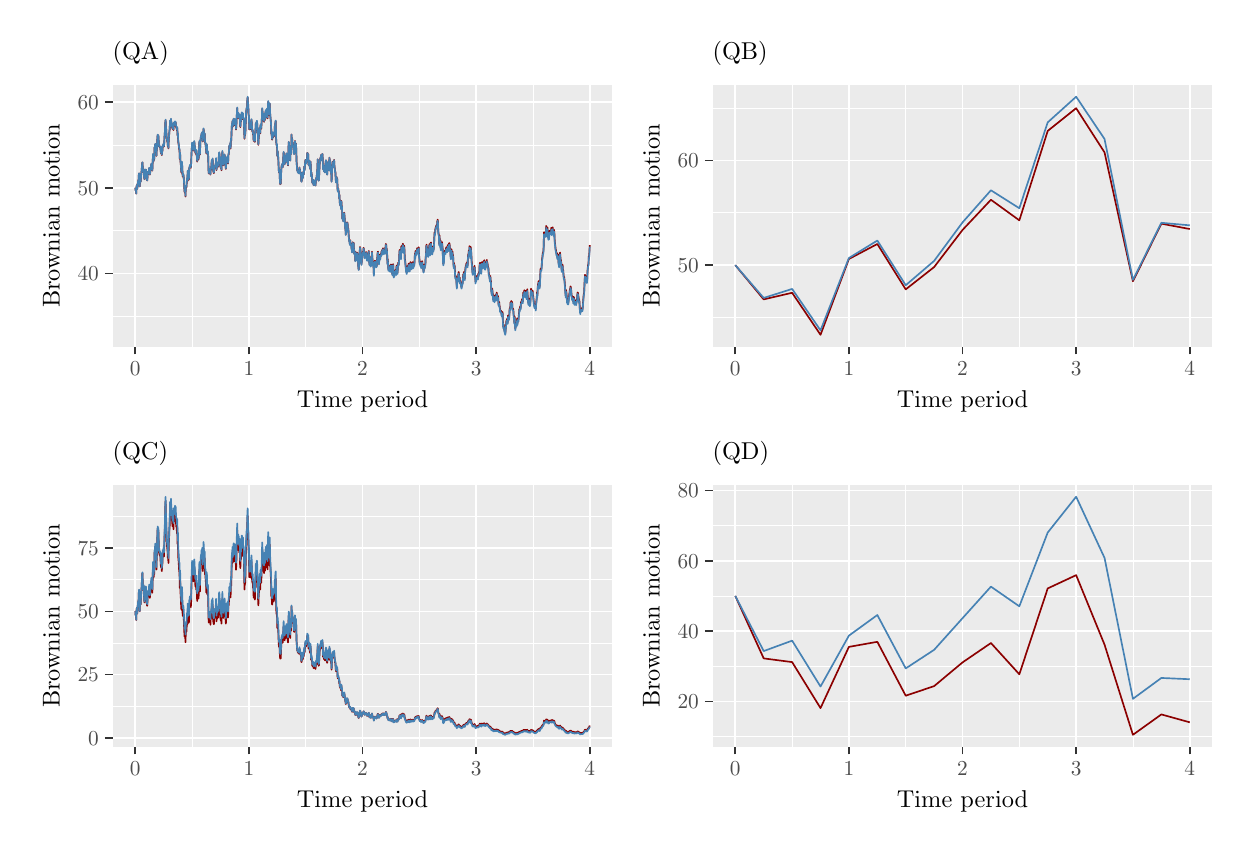
\begin{tikzpicture}[x=1pt,y=1pt]
\definecolor{fillColor}{RGB}{255,255,255}
\path[use as bounding box,fill=fillColor,fill opacity=0.00] (0,0) rectangle (433.62,289.08);
\begin{scope}
\path[clip] (  0.00,144.54) rectangle (216.81,289.08);
\definecolor{drawColor}{RGB}{255,255,255}
\definecolor{fillColor}{RGB}{255,255,255}

\path[draw=drawColor,line width= 0.6pt,line join=round,line cap=round,fill=fillColor] (  0.00,144.54) rectangle (216.81,289.08);
\end{scope}
\begin{scope}
\path[clip] ( 30.68,173.80) rectangle (211.31,268.42);
\definecolor{fillColor}{gray}{0.92}

\path[fill=fillColor] ( 30.68,173.80) rectangle (211.31,268.42);
\definecolor{drawColor}{RGB}{255,255,255}

\path[draw=drawColor,line width= 0.3pt,line join=round] ( 30.68,184.79) --
	(211.31,184.79);

\path[draw=drawColor,line width= 0.3pt,line join=round] ( 30.68,215.73) --
	(211.31,215.73);

\path[draw=drawColor,line width= 0.3pt,line join=round] ( 30.68,246.67) --
	(211.31,246.67);

\path[draw=drawColor,line width= 0.3pt,line join=round] ( 59.42,173.80) --
	( 59.42,268.42);

\path[draw=drawColor,line width= 0.3pt,line join=round] (100.47,173.80) --
	(100.47,268.42);

\path[draw=drawColor,line width= 0.3pt,line join=round] (141.52,173.80) --
	(141.52,268.42);

\path[draw=drawColor,line width= 0.3pt,line join=round] (182.57,173.80) --
	(182.57,268.42);

\path[draw=drawColor,line width= 0.6pt,line join=round] ( 30.68,200.26) --
	(211.31,200.26);

\path[draw=drawColor,line width= 0.6pt,line join=round] ( 30.68,231.20) --
	(211.31,231.20);

\path[draw=drawColor,line width= 0.6pt,line join=round] ( 30.68,262.13) --
	(211.31,262.13);

\path[draw=drawColor,line width= 0.6pt,line join=round] ( 38.89,173.80) --
	( 38.89,268.42);

\path[draw=drawColor,line width= 0.6pt,line join=round] ( 79.94,173.80) --
	( 79.94,268.42);

\path[draw=drawColor,line width= 0.6pt,line join=round] (121.00,173.80) --
	(121.00,268.42);

\path[draw=drawColor,line width= 0.6pt,line join=round] (162.05,173.80) --
	(162.05,268.42);

\path[draw=drawColor,line width= 0.6pt,line join=round] (203.10,173.80) --
	(203.10,268.42);
\definecolor{drawColor}{RGB}{139,0,0}

\path[draw=drawColor,line width= 0.6pt,line join=round] ( 38.89,231.20) --
	( 39.01,230.17) --
	( 39.12,230.46) --
	( 39.23,229.10) --
	( 39.35,231.68) --
	( 39.46,232.21) --
	( 39.58,230.86) --
	( 39.69,231.65) --
	( 39.80,232.85) --
	( 39.92,233.80) --
	( 40.03,233.28) --
	( 40.15,235.79) --
	( 40.26,236.44) --
	( 40.37,235.39) --
	( 40.49,231.71) --
	( 40.60,233.55) --
	( 40.72,233.47) --
	( 40.83,233.43) --
	( 40.94,234.99) --
	( 41.06,236.36) --
	( 41.17,237.36) --
	( 41.29,238.92) --
	( 41.40,240.25) --
	( 41.51,240.37) --
	( 41.63,236.96) --
	( 41.74,238.00) --
	( 41.86,237.90) --
	( 41.97,237.63) --
	( 42.08,235.14) --
	( 42.20,234.33) --
	( 42.31,235.02) --
	( 42.43,237.30) --
	( 42.54,237.11) --
	( 42.65,237.76) --
	( 42.77,237.66) --
	( 42.88,235.33) --
	( 43.00,234.63) --
	( 43.11,233.97) --
	( 43.22,233.86) --
	( 43.34,235.68) --
	( 43.45,236.96) --
	( 43.57,236.67) --
	( 43.68,236.24) --
	( 43.79,237.41) --
	( 43.91,238.34) --
	( 44.02,237.17) --
	( 44.14,235.96) --
	( 44.25,236.57) --
	( 44.36,237.86) --
	( 44.48,237.66) --
	( 44.59,239.16) --
	( 44.71,239.83) --
	( 44.82,238.77) --
	( 44.94,239.35) --
	( 45.05,237.41) --
	( 45.16,239.85) --
	( 45.28,243.29) --
	( 45.39,242.63) --
	( 45.51,240.81) --
	( 45.62,241.79) --
	( 45.73,241.54) --
	( 45.85,245.76) --
	( 45.96,245.68) --
	( 46.08,246.91) --
	( 46.19,246.95) --
	( 46.30,245.61) --
	( 46.42,245.94) --
	( 46.53,242.74) --
	( 46.65,245.31) --
	( 46.76,245.58) --
	( 46.87,249.48) --
	( 46.99,250.34) --
	( 47.10,249.04) --
	( 47.22,250.14) --
	( 47.33,248.43) --
	( 47.44,246.17) --
	( 47.56,246.68) --
	( 47.67,245.88) --
	( 47.79,245.87) --
	( 47.90,245.99) --
	( 48.01,244.93) --
	( 48.13,243.92) --
	( 48.24,243.67) --
	( 48.36,245.75) --
	( 48.47,243.04) --
	( 48.58,244.08) --
	( 48.70,244.66) --
	( 48.81,246.54) --
	( 48.93,245.99) --
	( 49.04,246.64) --
	( 49.15,247.11) --
	( 49.27,246.13) --
	( 49.38,248.30) --
	( 49.50,250.40) --
	( 49.61,251.68) --
	( 49.72,254.62) --
	( 49.84,255.66) --
	( 49.95,253.26) --
	( 50.07,252.19) --
	( 50.18,249.92) --
	( 50.29,249.05) --
	( 50.41,247.92) --
	( 50.52,247.98) --
	( 50.64,246.33) --
	( 50.75,246.61) --
	( 50.86,245.43) --
	( 50.98,248.60) --
	( 51.09,249.89) --
	( 51.21,251.55) --
	( 51.32,252.25) --
	( 51.44,255.39) --
	( 51.55,254.18) --
	( 51.66,253.31) --
	( 51.78,255.99) --
	( 51.89,254.75) --
	( 52.01,254.35) --
	( 52.12,253.61) --
	( 52.23,253.00) --
	( 52.35,252.47) --
	( 52.46,253.38) --
	( 52.58,253.04) --
	( 52.69,252.10) --
	( 52.80,254.59) --
	( 52.92,254.18) --
	( 53.03,253.83) --
	( 53.15,253.63) --
	( 53.26,254.96) --
	( 53.37,254.81) --
	( 53.49,254.73) --
	( 53.60,253.44) --
	( 53.72,252.83) --
	( 53.83,252.93) --
	( 53.94,251.83) --
	( 54.06,252.81) --
	( 54.17,250.00) --
	( 54.29,250.55) --
	( 54.40,247.74) --
	( 54.51,247.19) --
	( 54.63,246.24) --
	( 54.74,245.06) --
	( 54.86,244.95) --
	( 54.97,241.58) --
	( 55.08,243.63) --
	( 55.20,240.71) --
	( 55.31,239.90) --
	( 55.43,237.98) --
	( 55.54,236.70) --
	( 55.65,240.26) --
	( 55.77,240.28) --
	( 55.88,238.06) --
	( 56.00,235.28) --
	( 56.11,236.03) --
	( 56.22,235.99) --
	( 56.34,235.45) --
	( 56.45,233.89) --
	( 56.57,231.43) --
	( 56.68,229.68) --
	( 56.79,231.29) --
	( 56.91,230.27) --
	( 57.02,228.04) --
	( 57.14,231.05) --
	( 57.25,231.73) --
	( 57.36,231.33) --
	( 57.48,233.06) --
	( 57.59,234.52) --
	( 57.71,233.48) --
	( 57.82,237.17) --
	( 57.93,236.73) --
	( 58.05,234.33) --
	( 58.16,234.08) --
	( 58.28,234.42) --
	( 58.39,238.30) --
	( 58.51,238.47) --
	( 58.62,239.24) --
	( 58.73,239.10) --
	( 58.85,238.52) --
	( 58.96,238.45) --
	( 59.08,239.79) --
	( 59.19,243.40) --
	( 59.30,245.20) --
	( 59.42,247.36) --
	( 59.53,245.14) --
	( 59.65,246.89) --
	( 59.76,247.28) --
	( 59.87,244.65) --
	( 59.99,245.56) --
	( 60.10,245.27) --
	( 60.22,247.89) --
	( 60.33,246.50) --
	( 60.44,245.72) --
	( 60.56,244.07) --
	( 60.67,243.75) --
	( 60.79,244.45) --
	( 60.90,243.15) --
	( 61.01,244.60) --
	( 61.13,242.47) --
	( 61.24,240.64) --
	( 61.36,243.14) --
	( 61.47,241.36) --
	( 61.58,242.06) --
	( 61.70,241.39) --
	( 61.81,242.09) --
	( 61.93,245.06) --
	( 62.04,247.89) --
	( 62.15,247.29) --
	( 62.27,243.21) --
	( 62.38,247.65) --
	( 62.50,248.85) --
	( 62.61,249.82) --
	( 62.72,249.79) --
	( 62.84,250.71) --
	( 62.95,250.40) --
	( 63.07,251.17) --
	( 63.18,250.42) --
	( 63.29,247.92) --
	( 63.41,249.70) --
	( 63.52,252.49) --
	( 63.64,251.91) --
	( 63.75,249.60) --
	( 63.86,250.76) --
	( 63.98,250.67) --
	( 64.09,247.51) --
	( 64.21,247.50) --
	( 64.32,246.36) --
	( 64.43,245.74) --
	( 64.55,243.68) --
	( 64.66,246.88) --
	( 64.78,246.28) --
	( 64.89,243.42) --
	( 65.00,243.76) --
	( 65.12,244.21) --
	( 65.23,242.47) --
	( 65.35,237.48) --
	( 65.46,236.39) --
	( 65.58,237.35) --
	( 65.69,237.24) --
	( 65.80,237.06) --
	( 65.92,238.00) --
	( 66.03,235.99) --
	( 66.15,237.83) --
	( 66.26,237.82) --
	( 66.37,239.01) --
	( 66.49,240.79) --
	( 66.60,241.16) --
	( 66.72,239.64) --
	( 66.83,241.64) --
	( 66.94,238.19) --
	( 67.06,237.25) --
	( 67.17,236.81) --
	( 67.29,236.52) --
	( 67.40,238.24) --
	( 67.51,238.47) --
	( 67.63,239.15) --
	( 67.74,239.02) --
	( 67.86,238.59) --
	( 67.97,239.78) --
	( 68.08,241.75) --
	( 68.20,237.61) --
	( 68.31,238.58) --
	( 68.43,239.21) --
	( 68.54,238.47) --
	( 68.65,240.09) --
	( 68.77,239.41) --
	( 68.88,238.92) --
	( 69.00,240.38) --
	( 69.11,243.37) --
	( 69.22,243.84) --
	( 69.34,243.09) --
	( 69.45,241.00) --
	( 69.57,240.42) --
	( 69.68,238.80) --
	( 69.79,238.34) --
	( 69.91,239.01) --
	( 70.02,237.55) --
	( 70.14,242.10) --
	( 70.25,242.36) --
	( 70.36,244.34) --
	( 70.48,240.33) --
	( 70.59,241.61) --
	( 70.71,239.32) --
	( 70.82,240.90) --
	( 70.93,241.58) --
	( 71.05,240.86) --
	( 71.16,243.16) --
	( 71.28,241.93) --
	( 71.39,240.91) --
	( 71.50,239.18) --
	( 71.62,238.02) --
	( 71.73,239.63) --
	( 71.85,240.37) --
	( 71.96,242.11) --
	( 72.08,241.42) --
	( 72.19,242.07) --
	( 72.30,242.48) --
	( 72.42,240.00) --
	( 72.53,243.08) --
	( 72.65,243.31) --
	( 72.76,244.65) --
	( 72.87,246.34) --
	( 72.99,246.24) --
	( 73.10,245.69) --
	( 73.22,247.28) --
	( 73.33,245.39) --
	( 73.44,248.93) --
	( 73.56,248.23) --
	( 73.67,251.24) --
	( 73.79,254.03) --
	( 73.90,254.18) --
	( 74.01,255.23) --
	( 74.13,253.30) --
	( 74.24,253.90) --
	( 74.36,255.85) --
	( 74.47,256.03) --
	( 74.58,255.16) --
	( 74.70,253.92) --
	( 74.81,253.84) --
	( 74.93,255.84) --
	( 75.04,254.92) --
	( 75.15,254.68) --
	( 75.27,252.26) --
	( 75.38,253.17) --
	( 75.50,255.61) --
	( 75.61,258.45) --
	( 75.72,260.01) --
	( 75.84,256.42) --
	( 75.95,257.32) --
	( 76.07,258.18) --
	( 76.18,257.50) --
	( 76.29,257.81) --
	( 76.41,256.16) --
	( 76.52,257.44) --
	( 76.64,256.81) --
	( 76.75,253.84) --
	( 76.86,253.15) --
	( 76.98,255.69) --
	( 77.09,255.05) --
	( 77.21,256.43) --
	( 77.32,258.22) --
	( 77.43,258.22) --
	( 77.55,257.54) --
	( 77.66,256.52) --
	( 77.78,257.92) --
	( 77.89,255.89) --
	( 78.00,256.34) --
	( 78.12,255.78) --
	( 78.23,251.54) --
	( 78.35,248.96) --
	( 78.46,250.62) --
	( 78.57,250.26) --
	( 78.69,251.73) --
	( 78.80,255.24) --
	( 78.92,258.02) --
	( 79.03,259.32) --
	( 79.15,260.04) --
	( 79.26,259.66) --
	( 79.37,262.72) --
	( 79.49,263.88) --
	( 79.60,261.57) --
	( 79.72,261.25) --
	( 79.83,257.54) --
	( 79.94,257.16) --
	( 80.06,252.28) --
	( 80.17,254.72) --
	( 80.29,253.52) --
	( 80.40,252.71) --
	( 80.51,252.39) --
	( 80.63,253.52) --
	( 80.74,254.78) --
	( 80.86,255.84) --
	( 80.97,254.75) --
	( 81.08,252.20) --
	( 81.20,251.47) --
	( 81.31,251.97) --
	( 81.43,250.45) --
	( 81.54,250.31) --
	( 81.65,248.18) --
	( 81.77,248.15) --
	( 81.88,248.38) --
	( 82.00,248.10) --
	( 82.11,247.80) --
	( 82.22,251.00) --
	( 82.34,252.40) --
	( 82.45,254.46) --
	( 82.57,252.73) --
	( 82.68,253.02) --
	( 82.79,255.18) --
	( 82.91,255.06) --
	( 83.02,251.09) --
	( 83.14,251.71) --
	( 83.25,248.22) --
	( 83.36,246.75) --
	( 83.48,249.13) --
	( 83.59,250.25) --
	( 83.71,252.25) --
	( 83.82,252.81) --
	( 83.93,252.59) --
	( 84.05,250.88) --
	( 84.16,253.82) --
	( 84.28,253.89) --
	( 84.39,252.55) --
	( 84.50,254.15) --
	( 84.62,256.17) --
	( 84.73,259.78) --
	( 84.85,258.61) --
	( 84.96,257.85) --
	( 85.07,257.05) --
	( 85.19,256.33) --
	( 85.30,255.62) --
	( 85.42,255.05) --
	( 85.53,257.78) --
	( 85.65,256.44) --
	( 85.76,255.70) --
	( 85.87,256.92) --
	( 85.99,259.06) --
	( 86.10,257.57) --
	( 86.22,256.60) --
	( 86.33,257.58) --
	( 86.44,259.53) --
	( 86.56,259.03) --
	( 86.67,256.29) --
	( 86.79,259.55) --
	( 86.90,262.33) --
	( 87.01,260.93) --
	( 87.13,260.80) --
	( 87.24,257.40) --
	( 87.36,258.48) --
	( 87.47,261.59) --
	( 87.58,258.41) --
	( 87.70,256.91) --
	( 87.81,255.69) --
	( 87.93,254.40) --
	( 88.04,250.61) --
	( 88.15,251.53) --
	( 88.27,248.71) --
	( 88.38,248.66) --
	( 88.50,249.73) --
	( 88.61,249.36) --
	( 88.72,250.98) --
	( 88.84,250.92) --
	( 88.95,249.73) --
	( 89.07,250.90) --
	( 89.18,250.10) --
	( 89.29,253.36) --
	( 89.41,253.32) --
	( 89.52,254.90) --
	( 89.64,255.28) --
	( 89.75,249.69) --
	( 89.86,247.21) --
	( 89.98,246.43) --
	( 90.09,246.85) --
	( 90.21,242.69) --
	( 90.32,244.37) --
	( 90.43,243.29) --
	( 90.55,241.97) --
	( 90.66,239.27) --
	( 90.78,236.78) --
	( 90.89,236.87) --
	( 91.00,237.72) --
	( 91.12,234.19) --
	( 91.23,232.52) --
	( 91.35,233.39) --
	( 91.46,232.64) --
	( 91.57,236.23) --
	( 91.69,238.34) --
	( 91.80,239.35) --
	( 91.92,239.35) --
	( 92.03,239.82) --
	( 92.14,238.60) --
	( 92.26,239.66) --
	( 92.37,242.22) --
	( 92.49,244.11) --
	( 92.60,242.68) --
	( 92.72,239.85) --
	( 92.83,239.66) --
	( 92.94,240.41) --
	( 93.06,242.75) --
	( 93.17,240.45) --
	( 93.29,241.07) --
	( 93.40,241.46) --
	( 93.51,243.54) --
	( 93.63,243.48) --
	( 93.74,242.85) --
	( 93.86,240.84) --
	( 93.97,239.94) --
	( 94.08,239.31) --
	( 94.20,243.38) --
	( 94.31,247.73) --
	( 94.43,247.42) --
	( 94.54,245.54) --
	( 94.65,242.05) --
	( 94.77,242.94) --
	( 94.88,241.03) --
	( 95.00,245.03) --
	( 95.11,243.46) --
	( 95.22,243.64) --
	( 95.34,250.48) --
	( 95.45,248.45) --
	( 95.57,249.00) --
	( 95.68,246.99) --
	( 95.79,247.61) --
	( 95.91,246.03) --
	( 96.02,246.16) --
	( 96.14,245.62) --
	( 96.25,243.51) --
	( 96.36,243.53) --
	( 96.48,245.27) --
	( 96.59,248.12) --
	( 96.71,245.65) --
	( 96.82,245.19) --
	( 96.93,247.26) --
	( 97.05,245.25) --
	( 97.16,240.81) --
	( 97.28,239.18) --
	( 97.39,237.53) --
	( 97.50,237.60) --
	( 97.62,236.90) --
	( 97.73,237.29) --
	( 97.85,236.56) --
	( 97.96,237.19) --
	( 98.07,236.56) --
	( 98.19,238.57) --
	( 98.30,237.31) --
	( 98.42,237.79) --
	( 98.53,236.29) --
	( 98.64,236.63) --
	( 98.76,236.54) --
	( 98.87,233.71) --
	( 98.99,233.47) --
	( 99.10,235.42) --
	( 99.22,236.56) --
	( 99.33,236.79) --
	( 99.44,234.78) --
	( 99.56,236.73) --
	( 99.67,236.86) --
	( 99.79,236.09) --
	( 99.90,238.87) --
	(100.01,237.55) --
	(100.13,238.05) --
	(100.24,240.24) --
	(100.36,241.27) --
	(100.47,240.73) --
	(100.58,240.00) --
	(100.70,240.60) --
	(100.81,241.49) --
	(100.93,241.51) --
	(101.04,243.81) --
	(101.15,243.68) --
	(101.27,242.44) --
	(101.38,243.38) --
	(101.50,239.54) --
	(101.61,240.21) --
	(101.72,241.06) --
	(101.84,240.66) --
	(101.95,238.73) --
	(102.07,238.05) --
	(102.18,240.70) --
	(102.29,239.41) --
	(102.41,235.44) --
	(102.52,236.80) --
	(102.64,235.95) --
	(102.75,235.08) --
	(102.86,233.05) --
	(102.98,233.01) --
	(103.09,234.16) --
	(103.21,233.18) --
	(103.32,232.17) --
	(103.43,233.97) --
	(103.55,233.55) --
	(103.66,233.28) --
	(103.78,232.24) --
	(103.89,233.72) --
	(104.00,232.07) --
	(104.12,233.46) --
	(104.23,234.79) --
	(104.35,234.00) --
	(104.46,235.41) --
	(104.57,237.06) --
	(104.69,238.03) --
	(104.80,241.50) --
	(104.92,238.12) --
	(105.03,236.14) --
	(105.14,233.83) --
	(105.26,234.10) --
	(105.37,236.74) --
	(105.49,239.59) --
	(105.60,240.43) --
	(105.71,241.94) --
	(105.83,241.68) --
	(105.94,242.49) --
	(106.06,243.14) --
	(106.17,241.80) --
	(106.29,241.28) --
	(106.40,241.04) --
	(106.51,243.46) --
	(106.63,241.64) --
	(106.74,237.99) --
	(106.86,239.29) --
	(106.97,237.89) --
	(107.08,237.14) --
	(107.20,238.67) --
	(107.31,237.36) --
	(107.43,236.78) --
	(107.54,239.33) --
	(107.65,240.23) --
	(107.77,241.16) --
	(107.88,240.91) --
	(108.00,238.94) --
	(108.11,236.39) --
	(108.22,236.01) --
	(108.34,239.40) --
	(108.45,239.77) --
	(108.57,240.04) --
	(108.68,240.61) --
	(108.79,239.94) --
	(108.91,237.53) --
	(109.02,242.13) --
	(109.14,241.38) --
	(109.25,240.86) --
	(109.36,237.77) --
	(109.48,237.34) --
	(109.59,236.92) --
	(109.71,236.47) --
	(109.82,233.48) --
	(109.93,236.45) --
	(110.05,239.45) --
	(110.16,240.62) --
	(110.28,238.72) --
	(110.39,239.94) --
	(110.50,239.51) --
	(110.62,238.95) --
	(110.73,241.29) --
	(110.85,239.16) --
	(110.96,238.28) --
	(111.07,237.03) --
	(111.19,237.05) --
	(111.30,234.40) --
	(111.42,233.23) --
	(111.53,234.41) --
	(111.64,235.17) --
	(111.76,233.55) --
	(111.87,234.47) --
	(111.99,230.46) --
	(112.10,229.90) --
	(112.21,231.05) --
	(112.33,229.97) --
	(112.44,229.90) --
	(112.56,227.34) --
	(112.67,228.68) --
	(112.79,225.74) --
	(112.90,225.22) --
	(113.01,224.81) --
	(113.13,224.90) --
	(113.24,223.61) --
	(113.36,226.46) --
	(113.47,224.21) --
	(113.58,224.60) --
	(113.70,220.07) --
	(113.81,220.07) --
	(113.93,220.84) --
	(114.04,219.19) --
	(114.15,220.24) --
	(114.27,220.74) --
	(114.38,222.22) --
	(114.50,220.92) --
	(114.61,219.45) --
	(114.72,216.79) --
	(114.84,216.31) --
	(114.95,214.34) --
	(115.07,215.34) --
	(115.18,215.44) --
	(115.29,218.67) --
	(115.41,216.94) --
	(115.52,218.69) --
	(115.64,217.90) --
	(115.75,215.73) --
	(115.86,216.57) --
	(115.98,214.46) --
	(116.09,212.93) --
	(116.21,211.87) --
	(116.32,212.16) --
	(116.43,210.74) --
	(116.55,212.26) --
	(116.66,210.55) --
	(116.78,210.85) --
	(116.89,211.04) --
	(117.00,209.53) --
	(117.12,208.93) --
	(117.23,208.01) --
	(117.35,209.34) --
	(117.46,211.52) --
	(117.57,210.04) --
	(117.69,211.35) --
	(117.80,211.24) --
	(117.92,208.47) --
	(118.03,207.41) --
	(118.14,208.04) --
	(118.26,208.24) --
	(118.37,204.88) --
	(118.49,205.66) --
	(118.60,206.55) --
	(118.71,206.13) --
	(118.83,205.16) --
	(118.94,207.85) --
	(119.06,207.72) --
	(119.17,207.69) --
	(119.28,206.14) --
	(119.40,204.31) --
	(119.51,202.27) --
	(119.63,201.70) --
	(119.74,203.50) --
	(119.86,205.87) --
	(119.97,208.01) --
	(120.08,209.82) --
	(120.20,209.48) --
	(120.31,207.76) --
	(120.43,207.30) --
	(120.54,204.01) --
	(120.65,203.58) --
	(120.77,205.82) --
	(120.88,205.99) --
	(121.00,207.49) --
	(121.11,208.16) --
	(121.22,207.07) --
	(121.34,209.49) --
	(121.45,209.37) --
	(121.57,208.01) --
	(121.68,208.10) --
	(121.79,206.00) --
	(121.91,207.18) --
	(122.02,207.86) --
	(122.14,207.36) --
	(122.25,206.69) --
	(122.36,207.97) --
	(122.48,206.50) --
	(122.59,205.15) --
	(122.71,205.72) --
	(122.82,205.10) --
	(122.93,206.35) --
	(123.05,206.07) --
	(123.16,207.71) --
	(123.28,208.39) --
	(123.39,205.30) --
	(123.50,203.49) --
	(123.62,205.21) --
	(123.73,206.14) --
	(123.85,204.82) --
	(123.96,203.01) --
	(124.07,204.39) --
	(124.19,203.29) --
	(124.30,205.71) --
	(124.42,208.14) --
	(124.53,206.13) --
	(124.64,204.97) --
	(124.76,203.28) --
	(124.87,204.17) --
	(124.99,202.44) --
	(125.10,199.76) --
	(125.21,202.41) --
	(125.33,203.74) --
	(125.44,204.84) --
	(125.56,203.93) --
	(125.67,203.91) --
	(125.78,204.74) --
	(125.90,203.01) --
	(126.01,202.84) --
	(126.13,203.07) --
	(126.24,205.34) --
	(126.36,206.21) --
	(126.47,207.96) --
	(126.58,208.15) --
	(126.70,206.61) --
	(126.81,206.14) --
	(126.93,203.88) --
	(127.04,205.12) --
	(127.15,207.05) --
	(127.27,206.96) --
	(127.38,205.61) --
	(127.50,207.09) --
	(127.61,207.27) --
	(127.72,206.73) --
	(127.84,208.28) --
	(127.95,207.22) --
	(128.07,208.80) --
	(128.18,207.63) --
	(128.29,208.16) --
	(128.41,209.40) --
	(128.52,207.53) --
	(128.64,208.08) --
	(128.75,207.91) --
	(128.86,208.85) --
	(128.98,207.74) --
	(129.09,207.62) --
	(129.21,209.53) --
	(129.32,209.76) --
	(129.43,210.92) --
	(129.55,210.60) --
	(129.66,209.14) --
	(129.78,209.12) --
	(129.89,207.41) --
	(130.00,203.87) --
	(130.12,205.44) --
	(130.23,203.97) --
	(130.35,201.53) --
	(130.46,202.84) --
	(130.57,202.82) --
	(130.69,202.02) --
	(130.80,201.77) --
	(130.92,201.21) --
	(131.03,202.52) --
	(131.14,203.48) --
	(131.26,201.18) --
	(131.37,201.64) --
	(131.49,202.59) --
	(131.60,203.48) --
	(131.71,200.27) --
	(131.83,199.96) --
	(131.94,202.55) --
	(132.06,203.61) --
	(132.17,201.33) --
	(132.28,199.15) --
	(132.40,199.78) --
	(132.51,199.55) --
	(132.63,200.80) --
	(132.74,201.18) --
	(132.85,201.28) --
	(132.97,201.51) --
	(133.08,201.72) --
	(133.20,200.05) --
	(133.31,203.14) --
	(133.43,201.26) --
	(133.54,201.24) --
	(133.65,200.51) --
	(133.77,202.88) --
	(133.88,204.23) --
	(134.00,203.47) --
	(134.11,203.73) --
	(134.22,205.30) --
	(134.34,208.36) --
	(134.45,208.78) --
	(134.57,207.33) --
	(134.68,205.97) --
	(134.79,208.73) --
	(134.91,205.87) --
	(135.02,210.09) --
	(135.14,209.72) --
	(135.25,209.07) --
	(135.36,209.29) --
	(135.48,210.59) --
	(135.59,211.01) --
	(135.71,208.26) --
	(135.82,208.75) --
	(135.93,209.37) --
	(136.05,210.29) --
	(136.16,208.83) --
	(136.28,205.56) --
	(136.39,205.11) --
	(136.50,203.83) --
	(136.62,202.80) --
	(136.73,201.53) --
	(136.85,201.00) --
	(136.96,200.59) --
	(137.07,201.62) --
	(137.19,202.93) --
	(137.30,201.86) --
	(137.42,201.45) --
	(137.53,201.92) --
	(137.64,203.78) --
	(137.76,203.69) --
	(137.87,201.43) --
	(137.99,201.73) --
	(138.10,201.56) --
	(138.21,203.91) --
	(138.33,204.37) --
	(138.44,203.53) --
	(138.56,202.93) --
	(138.67,202.25) --
	(138.78,202.49) --
	(138.90,202.72) --
	(139.01,203.94) --
	(139.13,204.36) --
	(139.24,203.86) --
	(139.35,202.60) --
	(139.47,203.44) --
	(139.58,203.35) --
	(139.70,203.58) --
	(139.81,205.06) --
	(139.93,207.45) --
	(140.04,206.14) --
	(140.15,208.39) --
	(140.27,207.19) --
	(140.38,207.55) --
	(140.50,207.85) --
	(140.61,207.46) --
	(140.72,209.39) --
	(140.84,208.46) --
	(140.95,209.38) --
	(141.07,209.35) --
	(141.18,208.04) --
	(141.29,209.73) --
	(141.41,206.82) --
	(141.52,206.10) --
	(141.64,204.00) --
	(141.75,204.26) --
	(141.86,204.61) --
	(141.98,203.10) --
	(142.09,203.96) --
	(142.21,202.57) --
	(142.32,203.45) --
	(142.43,203.76) --
	(142.55,204.71) --
	(142.66,203.44) --
	(142.78,203.56) --
	(142.89,202.94) --
	(143.00,200.99) --
	(143.12,201.18) --
	(143.23,203.53) --
	(143.35,202.66) --
	(143.46,202.39) --
	(143.57,203.30) --
	(143.69,203.34) --
	(143.80,205.96) --
	(143.92,206.96) --
	(144.03,210.18) --
	(144.14,210.67) --
	(144.26,209.07) --
	(144.37,209.65) --
	(144.49,208.35) --
	(144.60,206.95) --
	(144.71,206.68) --
	(144.83,207.96) --
	(144.94,208.43) --
	(145.06,209.56) --
	(145.17,210.84) --
	(145.28,210.59) --
	(145.40,207.23) --
	(145.51,208.33) --
	(145.63,211.37) --
	(145.74,211.45) --
	(145.85,209.52) --
	(145.97,209.00) --
	(146.08,207.70) --
	(146.20,207.63) --
	(146.31,208.56) --
	(146.42,209.77) --
	(146.54,210.09) --
	(146.65,208.77) --
	(146.77,209.91) --
	(146.88,211.81) --
	(147.00,215.05) --
	(147.11,214.32) --
	(147.22,215.01) --
	(147.34,216.75) --
	(147.45,216.57) --
	(147.57,217.34) --
	(147.68,217.65) --
	(147.79,217.44) --
	(147.91,217.69) --
	(148.02,219.12) --
	(148.14,219.73) --
	(148.25,219.02) --
	(148.36,215.69) --
	(148.48,214.52) --
	(148.59,214.48) --
	(148.71,210.86) --
	(148.82,214.02) --
	(148.93,211.88) --
	(149.05,210.22) --
	(149.16,212.28) --
	(149.28,209.18) --
	(149.39,210.21) --
	(149.50,209.72) --
	(149.62,210.35) --
	(149.73,211.59) --
	(149.85,210.22) --
	(149.96,209.23) --
	(150.07,205.09) --
	(150.19,203.79) --
	(150.30,204.29) --
	(150.42,204.97) --
	(150.53,207.73) --
	(150.64,207.82) --
	(150.76,208.45) --
	(150.87,208.55) --
	(150.99,207.87) --
	(151.10,208.90) --
	(151.21,209.54) --
	(151.33,209.72) --
	(151.44,208.57) --
	(151.56,208.51) --
	(151.67,209.59) --
	(151.78,210.53) --
	(151.90,209.85) --
	(152.01,208.90) --
	(152.13,209.61) --
	(152.24,211.08) --
	(152.35,211.25) --
	(152.47,210.80) --
	(152.58,209.55) --
	(152.70,208.96) --
	(152.81,206.89) --
	(152.92,205.93) --
	(153.04,207.48) --
	(153.15,209.02) --
	(153.27,207.80) --
	(153.38,208.09) --
	(153.50,208.18) --
	(153.61,205.88) --
	(153.72,206.98) --
	(153.84,204.37) --
	(153.95,202.70) --
	(154.07,204.02) --
	(154.18,203.29) --
	(154.29,203.00) --
	(154.41,200.85) --
	(154.52,198.95) --
	(154.64,199.40) --
	(154.75,199.17) --
	(154.86,198.40) --
	(154.98,196.69) --
	(155.09,195.30) --
	(155.21,197.87) --
	(155.32,197.45) --
	(155.43,198.43) --
	(155.55,199.44) --
	(155.66,200.42) --
	(155.78,200.80) --
	(155.89,199.16) --
	(156.00,197.86) --
	(156.12,198.82) --
	(156.23,197.14) --
	(156.35,197.80) --
	(156.46,197.11) --
	(156.57,196.60) --
	(156.69,195.60) --
	(156.80,195.31) --
	(156.92,196.40) --
	(157.03,196.97) --
	(157.14,196.67) --
	(157.26,197.77) --
	(157.37,199.90) --
	(157.49,199.88) --
	(157.60,200.49) --
	(157.71,200.85) --
	(157.83,199.56) --
	(157.94,198.36) --
	(158.06,200.85) --
	(158.17,202.00) --
	(158.28,202.98) --
	(158.40,203.17) --
	(158.51,203.81) --
	(158.63,204.01) --
	(158.74,204.06) --
	(158.85,204.35) --
	(158.97,202.99) --
	(159.08,206.22) --
	(159.20,207.32) --
	(159.31,206.96) --
	(159.42,208.63) --
	(159.54,207.76) --
	(159.65,210.14) --
	(159.77,209.58) --
	(159.88,206.35) --
	(159.99,208.23) --
	(160.11,209.80) --
	(160.22,208.71) --
	(160.34,206.75) --
	(160.45,204.25) --
	(160.57,203.88) --
	(160.68,201.44) --
	(160.79,200.36) --
	(160.91,200.57) --
	(161.02,201.68) --
	(161.14,200.60) --
	(161.25,200.43) --
	(161.36,200.76) --
	(161.48,203.02) --
	(161.59,201.74) --
	(161.71,199.64) --
	(161.82,197.26) --
	(161.93,197.96) --
	(162.05,197.88) --
	(162.16,198.86) --
	(162.28,198.67) --
	(162.39,199.17) --
	(162.50,199.46) --
	(162.62,199.48) --
	(162.73,198.67) --
	(162.85,200.30) --
	(162.96,199.76) --
	(163.07,200.63) --
	(163.19,200.83) --
	(163.30,203.18) --
	(163.42,204.13) --
	(163.53,203.67) --
	(163.64,203.65) --
	(163.76,203.48) --
	(163.87,200.70) --
	(163.99,202.94) --
	(164.10,204.35) --
	(164.21,203.32) --
	(164.33,203.82) --
	(164.44,204.14) --
	(164.56,202.62) --
	(164.67,204.61) --
	(164.78,204.27) --
	(164.90,204.51) --
	(165.01,205.05) --
	(165.13,203.70) --
	(165.24,202.25) --
	(165.35,202.18) --
	(165.47,202.93) --
	(165.58,203.02) --
	(165.70,203.96) --
	(165.81,204.41) --
	(165.92,205.14) --
	(166.04,203.24) --
	(166.15,204.14) --
	(166.27,203.08) --
	(166.38,202.45) --
	(166.49,202.30) --
	(166.61,200.13) --
	(166.72,199.99) --
	(166.84,199.42) --
	(166.95,198.48) --
	(167.06,197.76) --
	(167.18,199.36) --
	(167.29,197.73) --
	(167.41,197.45) --
	(167.52,194.34) --
	(167.64,193.49) --
	(167.75,192.87) --
	(167.86,194.77) --
	(167.98,193.57) --
	(168.09,192.50) --
	(168.21,190.79) --
	(168.32,191.00) --
	(168.43,192.40) --
	(168.55,190.94) --
	(168.66,190.42) --
	(168.78,192.06) --
	(168.89,191.23) --
	(169.00,192.05) --
	(169.12,192.52) --
	(169.23,190.93) --
	(169.35,192.40) --
	(169.46,193.37) --
	(169.57,192.76) --
	(169.69,191.65) --
	(169.80,191.18) --
	(169.92,192.16) --
	(170.03,191.46) --
	(170.14,189.21) --
	(170.26,189.03) --
	(170.37,189.95) --
	(170.49,188.56) --
	(170.60,188.28) --
	(170.71,186.84) --
	(170.83,186.97) --
	(170.94,186.81) --
	(171.06,186.76) --
	(171.17,186.04) --
	(171.28,185.21) --
	(171.40,186.21) --
	(171.51,186.33) --
	(171.63,186.11) --
	(171.74,182.45) --
	(171.85,181.03) --
	(171.97,181.87) --
	(172.08,181.41) --
	(172.20,180.08) --
	(172.31,179.59) --
	(172.42,179.18) --
	(172.54,178.63) --
	(172.65,179.16) --
	(172.77,180.82) --
	(172.88,181.90) --
	(172.99,183.29) --
	(173.11,182.91) --
	(173.22,183.86) --
	(173.34,182.75) --
	(173.45,182.59) --
	(173.56,185.05) --
	(173.68,185.03) --
	(173.79,184.68) --
	(173.91,184.01) --
	(174.02,184.88) --
	(174.14,187.31) --
	(174.25,187.78) --
	(174.36,187.47) --
	(174.48,189.91) --
	(174.59,188.98) --
	(174.71,190.32) --
	(174.82,189.81) --
	(174.93,188.59) --
	(175.05,190.04) --
	(175.16,187.90) --
	(175.28,187.53) --
	(175.39,187.54) --
	(175.50,187.02) --
	(175.62,185.12) --
	(175.73,184.38) --
	(175.85,182.62) --
	(175.96,184.79) --
	(176.07,182.68) --
	(176.19,180.35) --
	(176.30,181.11) --
	(176.42,182.11) --
	(176.53,181.88) --
	(176.64,181.65) --
	(176.76,182.45) --
	(176.87,184.02) --
	(176.99,182.22) --
	(177.10,183.68) --
	(177.21,183.90) --
	(177.33,183.51) --
	(177.44,184.94) --
	(177.56,186.01) --
	(177.67,187.49) --
	(177.78,187.14) --
	(177.90,188.05) --
	(178.01,188.39) --
	(178.13,187.77) --
	(178.24,189.85) --
	(178.35,190.03) --
	(178.47,189.96) --
	(178.58,190.59) --
	(178.70,191.05) --
	(178.81,190.20) --
	(178.92,190.13) --
	(179.04,193.29) --
	(179.15,193.19) --
	(179.27,192.82) --
	(179.38,193.72) --
	(179.49,194.21) --
	(179.61,193.54) --
	(179.72,192.20) --
	(179.84,193.23) --
	(179.95,193.37) --
	(180.06,193.96) --
	(180.18,193.60) --
	(180.29,191.57) --
	(180.41,191.65) --
	(180.52,194.58) --
	(180.63,192.77) --
	(180.75,191.56) --
	(180.86,189.94) --
	(180.98,189.50) --
	(181.09,191.15) --
	(181.21,190.96) --
	(181.32,190.65) --
	(181.43,189.10) --
	(181.55,189.17) --
	(181.66,190.40) --
	(181.78,193.14) --
	(181.89,194.76) --
	(182.00,193.68) --
	(182.12,193.05) --
	(182.23,193.79) --
	(182.35,193.77) --
	(182.46,194.11) --
	(182.57,192.49) --
	(182.69,191.96) --
	(182.80,190.83) --
	(182.92,189.71) --
	(183.03,188.85) --
	(183.14,188.35) --
	(183.26,188.34) --
	(183.37,189.08) --
	(183.49,188.47) --
	(183.60,187.46) --
	(183.71,189.36) --
	(183.83,190.54) --
	(183.94,191.38) --
	(184.06,193.45) --
	(184.17,192.24) --
	(184.28,194.76) --
	(184.40,196.29) --
	(184.51,196.68) --
	(184.63,197.46) --
	(184.74,197.53) --
	(184.85,197.39) --
	(184.97,195.39) --
	(185.08,196.32) --
	(185.20,199.05) --
	(185.31,201.77) --
	(185.42,201.98) --
	(185.54,201.84) --
	(185.65,202.07) --
	(185.77,203.59) --
	(185.88,205.57) --
	(185.99,206.12) --
	(186.11,207.65) --
	(186.22,207.60) --
	(186.34,208.28) --
	(186.45,209.93) --
	(186.56,215.14) --
	(186.68,215.06) --
	(186.79,214.08) --
	(186.91,214.72) --
	(187.02,214.12) --
	(187.13,215.04) --
	(187.25,215.53) --
	(187.36,217.46) --
	(187.48,216.04) --
	(187.59,214.27) --
	(187.71,216.55) --
	(187.82,216.88) --
	(187.93,215.51) --
	(188.05,213.94) --
	(188.16,213.14) --
	(188.28,213.98) --
	(188.39,213.21) --
	(188.50,215.15) --
	(188.62,215.50) --
	(188.73,215.78) --
	(188.85,215.75) --
	(188.96,215.31) --
	(189.07,215.05) --
	(189.19,216.75) --
	(189.30,214.77) --
	(189.42,216.36) --
	(189.53,215.83) --
	(189.64,216.91) --
	(189.76,216.81) --
	(189.87,214.83) --
	(189.99,215.33) --
	(190.10,214.39) --
	(190.21,216.03) --
	(190.33,214.81) --
	(190.44,212.22) --
	(190.56,211.00) --
	(190.67,210.18) --
	(190.78,209.01) --
	(190.90,208.67) --
	(191.01,207.84) --
	(191.13,207.27) --
	(191.24,207.71) --
	(191.35,206.10) --
	(191.47,207.14) --
	(191.58,207.13) --
	(191.70,207.07) --
	(191.81,204.29) --
	(191.92,203.88) --
	(192.04,203.13) --
	(192.15,204.26) --
	(192.27,206.14) --
	(192.38,207.82) --
	(192.49,206.28) --
	(192.61,205.19) --
	(192.72,205.06) --
	(192.84,203.63) --
	(192.95,201.49) --
	(193.06,202.53) --
	(193.18,202.61) --
	(193.29,203.42) --
	(193.41,201.82) --
	(193.52,201.36) --
	(193.63,199.82) --
	(193.75,198.74) --
	(193.86,199.03) --
	(193.98,197.98) --
	(194.09,196.71) --
	(194.20,195.06) --
	(194.32,193.27) --
	(194.43,192.21) --
	(194.55,194.30) --
	(194.66,193.48) --
	(194.78,192.11) --
	(194.89,190.40) --
	(195.00,190.22) --
	(195.12,189.74) --
	(195.23,190.03) --
	(195.35,189.69) --
	(195.46,190.72) --
	(195.57,191.59) --
	(195.69,192.87) --
	(195.80,193.16) --
	(195.92,194.53) --
	(196.03,194.43) --
	(196.14,195.59) --
	(196.26,195.38) --
	(196.37,194.53) --
	(196.49,193.01) --
	(196.60,192.14) --
	(196.71,191.22) --
	(196.83,191.92) --
	(196.94,191.85) --
	(197.06,191.08) --
	(197.17,189.99) --
	(197.28,191.81) --
	(197.40,191.51) --
	(197.51,190.00) --
	(197.63,189.48) --
	(197.74,189.59) --
	(197.85,190.58) --
	(197.97,190.47) --
	(198.08,190.60) --
	(198.20,189.35) --
	(198.31,190.29) --
	(198.42,190.41) --
	(198.54,191.29) --
	(198.65,193.17) --
	(198.77,193.38) --
	(198.88,193.03) --
	(198.99,192.08) --
	(199.11,191.38) --
	(199.22,190.27) --
	(199.34,190.71) --
	(199.45,188.95) --
	(199.56,186.89) --
	(199.68,186.11) --
	(199.79,187.37) --
	(199.91,187.50) --
	(200.02,186.92) --
	(200.13,187.70) --
	(200.25,187.28) --
	(200.36,187.14) --
	(200.48,187.22) --
	(200.59,188.49) --
	(200.70,190.02) --
	(200.82,191.56) --
	(200.93,192.75) --
	(201.05,193.14) --
	(201.16,195.47) --
	(201.28,198.05) --
	(201.39,199.76) --
	(201.50,199.47) --
	(201.62,198.12) --
	(201.73,198.36) --
	(201.85,197.64) --
	(201.96,197.99) --
	(202.07,197.28) --
	(202.19,198.45) --
	(202.30,201.29) --
	(202.42,202.56) --
	(202.53,203.54) --
	(202.64,203.58) --
	(202.76,206.53) --
	(202.87,206.41) --
	(202.99,208.31) --
	(203.10,210.50);
\definecolor{drawColor}{RGB}{70,130,180}

\path[draw=drawColor,line width= 0.6pt,line join=round] ( 38.89,231.20) --
	( 39.01,230.18) --
	( 39.12,230.47) --
	( 39.23,229.12) --
	( 39.35,231.68) --
	( 39.46,232.22) --
	( 39.58,230.88) --
	( 39.69,231.67) --
	( 39.80,232.88) --
	( 39.92,233.83) --
	( 40.03,233.32) --
	( 40.15,235.82) --
	( 40.26,236.47) --
	( 40.37,235.42) --
	( 40.49,231.72) --
	( 40.60,233.56) --
	( 40.72,233.48) --
	( 40.83,233.45) --
	( 40.94,235.02) --
	( 41.06,236.39) --
	( 41.17,237.39) --
	( 41.29,238.95) --
	( 41.40,240.29) --
	( 41.51,240.41) --
	( 41.63,236.98) --
	( 41.74,238.03) --
	( 41.86,237.93) --
	( 41.97,237.67) --
	( 42.08,235.17) --
	( 42.20,234.37) --
	( 42.31,235.06) --
	( 42.43,237.33) --
	( 42.54,237.16) --
	( 42.65,237.82) --
	( 42.77,237.72) --
	( 42.88,235.39) --
	( 43.00,234.69) --
	( 43.11,234.03) --
	( 43.22,233.94) --
	( 43.34,235.76) --
	( 43.45,237.04) --
	( 43.57,236.76) --
	( 43.68,236.33) --
	( 43.79,237.51) --
	( 43.91,238.45) --
	( 44.02,237.28) --
	( 44.14,236.08) --
	( 44.25,236.69) --
	( 44.36,237.99) --
	( 44.48,237.80) --
	( 44.59,239.29) --
	( 44.71,239.98) --
	( 44.82,238.92) --
	( 44.94,239.51) --
	( 45.05,237.57) --
	( 45.16,240.00) --
	( 45.28,243.41) --
	( 45.39,242.76) --
	( 45.51,240.93) --
	( 45.62,241.92) --
	( 45.73,241.69) --
	( 45.85,245.86) --
	( 45.96,245.79) --
	( 46.08,247.02) --
	( 46.19,247.07) --
	( 46.30,245.74) --
	( 46.42,246.07) --
	( 46.53,242.85) --
	( 46.65,245.42) --
	( 46.76,245.69) --
	( 46.87,249.56) --
	( 46.99,250.43) --
	( 47.10,249.13) --
	( 47.22,250.24) --
	( 47.33,248.53) --
	( 47.44,246.26) --
	( 47.56,246.78) --
	( 47.67,245.98) --
	( 47.79,245.99) --
	( 47.90,246.12) --
	( 48.01,245.07) --
	( 48.13,244.06) --
	( 48.24,243.82) --
	( 48.36,245.89) --
	( 48.47,243.18) --
	( 48.58,244.22) --
	( 48.70,244.81) --
	( 48.81,246.69) --
	( 48.93,246.15) --
	( 49.04,246.81) --
	( 49.15,247.29) --
	( 49.27,246.31) --
	( 49.38,248.47) --
	( 49.50,250.57) --
	( 49.61,251.85) --
	( 49.72,254.78) --
	( 49.84,255.83) --
	( 49.95,253.42) --
	( 50.07,252.35) --
	( 50.18,250.09) --
	( 50.29,249.22) --
	( 50.41,248.09) --
	( 50.52,248.17) --
	( 50.64,246.52) --
	( 50.75,246.81) --
	( 50.86,245.63) --
	( 50.98,248.78) --
	( 51.09,250.08) --
	( 51.21,251.74) --
	( 51.32,252.45) --
	( 51.44,255.57) --
	( 51.55,254.37) --
	( 51.66,253.50) --
	( 51.78,256.17) --
	( 51.89,254.94) --
	( 52.01,254.55) --
	( 52.12,253.82) --
	( 52.23,253.22) --
	( 52.35,252.70) --
	( 52.46,253.62) --
	( 52.58,253.28) --
	( 52.69,252.34) --
	( 52.80,254.83) --
	( 52.92,254.43) --
	( 53.03,254.09) --
	( 53.15,253.90) --
	( 53.26,255.23) --
	( 53.37,255.09) --
	( 53.49,255.02) --
	( 53.60,253.74) --
	( 53.72,253.14) --
	( 53.83,253.25) --
	( 53.94,252.16) --
	( 54.06,253.14) --
	( 54.17,250.32) --
	( 54.29,250.88) --
	( 54.40,248.06) --
	( 54.51,247.52) --
	( 54.63,246.56) --
	( 54.74,245.40) --
	( 54.86,245.30) --
	( 54.97,241.90) --
	( 55.08,243.95) --
	( 55.20,241.01) --
	( 55.31,240.21) --
	( 55.43,238.29) --
	( 55.54,237.01) --
	( 55.65,240.53) --
	( 55.77,240.56) --
	( 55.88,238.34) --
	( 56.00,235.55) --
	( 56.11,236.30) --
	( 56.22,236.27) --
	( 56.34,235.74) --
	( 56.45,234.18) --
	( 56.57,231.71) --
	( 56.68,229.96) --
	( 56.79,231.57) --
	( 56.91,230.56) --
	( 57.02,228.31) --
	( 57.14,231.30) --
	( 57.25,231.99) --
	( 57.36,231.60) --
	( 57.48,233.33) --
	( 57.59,234.79) --
	( 57.71,233.76) --
	( 57.82,237.41) --
	( 57.93,236.98) --
	( 58.05,234.57) --
	( 58.16,234.33) --
	( 58.28,234.68) --
	( 58.39,238.52) --
	( 58.51,238.70) --
	( 58.62,239.48) --
	( 58.73,239.35) --
	( 58.85,238.78) --
	( 58.96,238.72) --
	( 59.08,240.06) --
	( 59.19,243.63) --
	( 59.30,245.44) --
	( 59.42,247.59) --
	( 59.53,245.37) --
	( 59.65,247.12) --
	( 59.76,247.51) --
	( 59.87,244.87) --
	( 59.99,245.80) --
	( 60.10,245.51) --
	( 60.22,248.12) --
	( 60.33,246.73) --
	( 60.44,245.96) --
	( 60.56,244.31) --
	( 60.67,244.00) --
	( 60.79,244.71) --
	( 60.90,243.41) --
	( 61.01,244.87) --
	( 61.13,242.73) --
	( 61.24,240.90) --
	( 61.36,243.39) --
	( 61.47,241.61) --
	( 61.58,242.32) --
	( 61.70,241.66) --
	( 61.81,242.37) --
	( 61.93,245.32) --
	( 62.04,248.14) --
	( 62.15,247.54) --
	( 62.27,243.42) --
	( 62.38,247.81) --
	( 62.50,249.02) --
	( 62.61,250.00) --
	( 62.72,249.97) --
	( 62.84,250.91) --
	( 62.95,250.60) --
	( 63.07,251.38) --
	( 63.18,250.64) --
	( 63.29,248.13) --
	( 63.41,249.91) --
	( 63.52,252.69) --
	( 63.64,252.11) --
	( 63.75,249.80) --
	( 63.86,250.97) --
	( 63.98,250.89) --
	( 64.09,247.70) --
	( 64.21,247.71) --
	( 64.32,246.57) --
	( 64.43,245.96) --
	( 64.55,243.90) --
	( 64.66,247.08) --
	( 64.78,246.48) --
	( 64.89,243.61) --
	( 65.00,243.96) --
	( 65.12,244.42) --
	( 65.23,242.68) --
	( 65.35,237.62) --
	( 65.46,236.54) --
	( 65.58,237.50) --
	( 65.69,237.40) --
	( 65.80,237.23) --
	( 65.92,238.18) --
	( 66.03,236.16) --
	( 66.15,238.00) --
	( 66.26,237.99) --
	( 66.37,239.20) --
	( 66.49,240.97) --
	( 66.60,241.35) --
	( 66.72,239.83) --
	( 66.83,241.83) --
	( 66.94,238.35) --
	( 67.06,237.42) --
	( 67.17,236.99) --
	( 67.29,236.71) --
	( 67.40,238.43) --
	( 67.51,238.66) --
	( 67.63,239.35) --
	( 67.74,239.23) --
	( 67.86,238.81) --
	( 67.97,240.00) --
	( 68.08,241.97) --
	( 68.20,237.79) --
	( 68.31,238.76) --
	( 68.43,239.40) --
	( 68.54,238.67) --
	( 68.65,240.29) --
	( 68.77,239.62) --
	( 68.88,239.13) --
	( 69.00,240.60) --
	( 69.11,243.57) --
	( 69.22,244.05) --
	( 69.34,243.30) --
	( 69.45,241.21) --
	( 69.57,240.64) --
	( 69.68,239.02) --
	( 69.79,238.57) --
	( 69.91,239.25) --
	( 70.02,237.79) --
	( 70.14,242.28) --
	( 70.25,242.56) --
	( 70.36,244.53) --
	( 70.48,240.48) --
	( 70.59,241.76) --
	( 70.71,239.47) --
	( 70.82,241.05) --
	( 70.93,241.74) --
	( 71.05,241.03) --
	( 71.16,243.32) --
	( 71.28,242.09) --
	( 71.39,241.08) --
	( 71.50,239.35) --
	( 71.62,238.20) --
	( 71.73,239.81) --
	( 71.85,240.56) --
	( 71.96,242.29) --
	( 72.08,241.61) --
	( 72.19,242.26) --
	( 72.30,242.69) --
	( 72.42,240.20) --
	( 72.53,243.26) --
	( 72.65,243.50) --
	( 72.76,244.84) --
	( 72.87,246.54) --
	( 72.99,246.44) --
	( 73.10,245.90) --
	( 73.22,247.49) --
	( 73.33,245.61) --
	( 73.44,249.12) --
	( 73.56,248.42) --
	( 73.67,251.41) --
	( 73.79,254.20) --
	( 73.90,254.35) --
	( 74.01,255.41) --
	( 74.13,253.48) --
	( 74.24,254.09) --
	( 74.36,256.04) --
	( 74.47,256.22) --
	( 74.58,255.37) --
	( 74.70,254.13) --
	( 74.81,254.06) --
	( 74.93,256.06) --
	( 75.04,255.15) --
	( 75.15,254.92) --
	( 75.27,252.49) --
	( 75.38,253.40) --
	( 75.50,255.84) --
	( 75.61,258.67) --
	( 75.72,260.23) --
	( 75.84,256.61) --
	( 75.95,257.53) --
	( 76.07,258.40) --
	( 76.18,257.72) --
	( 76.29,258.04) --
	( 76.41,256.39) --
	( 76.52,257.68) --
	( 76.64,257.06) --
	( 76.75,254.07) --
	( 76.86,253.39) --
	( 76.98,255.93) --
	( 77.09,255.30) --
	( 77.21,256.67) --
	( 77.32,258.47) --
	( 77.43,258.48) --
	( 77.55,257.80) --
	( 77.66,256.79) --
	( 77.78,258.20) --
	( 77.89,256.16) --
	( 78.00,256.63) --
	( 78.12,256.08) --
	( 78.23,251.80) --
	( 78.35,249.20) --
	( 78.46,250.86) --
	( 78.57,250.51) --
	( 78.69,251.99) --
	( 78.80,255.47) --
	( 78.92,258.25) --
	( 79.03,259.54) --
	( 79.15,260.28) --
	( 79.26,259.90) --
	( 79.37,262.95) --
	( 79.49,264.12) --
	( 79.60,261.80) --
	( 79.72,261.50) --
	( 79.83,257.76) --
	( 79.94,257.39) --
	( 80.06,252.45) --
	( 80.17,254.89) --
	( 80.29,253.69) --
	( 80.40,252.89) --
	( 80.51,252.58) --
	( 80.63,253.71) --
	( 80.74,254.98) --
	( 80.86,256.04) --
	( 80.97,254.96) --
	( 81.08,252.40) --
	( 81.20,251.68) --
	( 81.31,252.19) --
	( 81.43,250.67) --
	( 81.54,250.54) --
	( 81.65,248.41) --
	( 81.77,248.39) --
	( 81.88,248.62) --
	( 82.00,248.36) --
	( 82.11,248.06) --
	( 82.22,251.25) --
	( 82.34,252.65) --
	( 82.45,254.71) --
	( 82.57,252.98) --
	( 82.68,253.28) --
	( 82.79,255.43) --
	( 82.91,255.33) --
	( 83.02,251.32) --
	( 83.14,251.95) --
	( 83.25,248.43) --
	( 83.36,246.97) --
	( 83.48,249.34) --
	( 83.59,250.46) --
	( 83.71,252.46) --
	( 83.82,253.03) --
	( 83.93,252.82) --
	( 84.05,251.11) --
	( 84.16,254.04) --
	( 84.28,254.12) --
	( 84.39,252.78) --
	( 84.50,254.39) --
	( 84.62,256.40) --
	( 84.73,259.99) --
	( 84.85,258.83) --
	( 84.96,258.08) --
	( 85.07,257.28) --
	( 85.19,256.57) --
	( 85.30,255.87) --
	( 85.42,255.31) --
	( 85.53,258.03) --
	( 85.65,256.69) --
	( 85.76,255.96) --
	( 85.87,257.19) --
	( 85.99,259.33) --
	( 86.10,257.84) --
	( 86.22,256.87) --
	( 86.33,257.87) --
	( 86.44,259.81) --
	( 86.56,259.32) --
	( 86.67,256.57) --
	( 86.79,259.81) --
	( 86.90,262.58) --
	( 87.01,261.19) --
	( 87.13,261.06) --
	( 87.24,257.65) --
	( 87.36,258.73) --
	( 87.47,261.82) --
	( 87.58,258.63) --
	( 87.70,257.14) --
	( 87.81,255.92) --
	( 87.93,254.63) --
	( 88.04,250.82) --
	( 88.15,251.74) --
	( 88.27,248.91) --
	( 88.38,248.87) --
	( 88.50,249.94) --
	( 88.61,249.58) --
	( 88.72,251.21) --
	( 88.84,251.16) --
	( 88.95,249.97) --
	( 89.07,251.15) --
	( 89.18,250.35) --
	( 89.29,253.59) --
	( 89.41,253.56) --
	( 89.52,255.15) --
	( 89.64,255.53) --
	( 89.75,249.87) --
	( 89.86,247.37) --
	( 89.98,246.61) --
	( 90.09,247.03) --
	( 90.21,242.83) --
	( 90.32,244.51) --
	( 90.43,243.44) --
	( 90.55,242.12) --
	( 90.66,239.41) --
	( 90.78,236.91) --
	( 90.89,237.01) --
	( 91.00,237.87) --
	( 91.12,234.30) --
	( 91.23,232.63) --
	( 91.35,233.51) --
	( 91.46,232.77) --
	( 91.57,236.33) --
	( 91.69,238.43) --
	( 91.80,239.44) --
	( 91.92,239.45) --
	( 92.03,239.93) --
	( 92.14,238.71) --
	( 92.26,239.79) --
	( 92.37,242.33) --
	( 92.49,244.23) --
	( 92.60,242.79) --
	( 92.72,239.95) --
	( 92.83,239.76) --
	( 92.94,240.52) --
	( 93.06,242.86) --
	( 93.17,240.55) --
	( 93.29,241.18) --
	( 93.40,241.58) --
	( 93.51,243.66) --
	( 93.63,243.61) --
	( 93.74,242.98) --
	( 93.86,240.97) --
	( 93.97,240.07) --
	( 94.08,239.45) --
	( 94.20,243.48) --
	( 94.31,247.78) --
	( 94.43,247.48) --
	( 94.54,245.60) --
	( 94.65,242.09) --
	( 94.77,242.99) --
	( 94.88,241.07) --
	( 95.00,245.04) --
	( 95.11,243.46) --
	( 95.22,243.66) --
	( 95.34,250.37) --
	( 95.45,248.34) --
	( 95.57,248.89) --
	( 95.68,246.88) --
	( 95.79,247.51) --
	( 95.91,245.93) --
	( 96.02,246.07) --
	( 96.14,245.54) --
	( 96.25,243.43) --
	( 96.36,243.45) --
	( 96.48,245.20) --
	( 96.59,248.03) --
	( 96.71,245.55) --
	( 96.82,245.10) --
	( 96.93,247.16) --
	( 97.05,245.16) --
	( 97.16,240.66) --
	( 97.28,239.04) --
	( 97.39,237.38) --
	( 97.50,237.46) --
	( 97.62,236.78) --
	( 97.73,237.17) --
	( 97.85,236.45) --
	( 97.96,237.08) --
	( 98.07,236.46) --
	( 98.19,238.47) --
	( 98.30,237.21) --
	( 98.42,237.70) --
	( 98.53,236.20) --
	( 98.64,236.55) --
	( 98.76,236.47) --
	( 98.87,233.63) --
	( 98.99,233.39) --
	( 99.10,235.34) --
	( 99.22,236.48) --
	( 99.33,236.73) --
	( 99.44,234.71) --
	( 99.56,236.66) --
	( 99.67,236.80) --
	( 99.79,236.03) --
	( 99.90,238.79) --
	(100.01,237.48) --
	(100.13,237.99) --
	(100.24,240.17) --
	(100.36,241.21) --
	(100.47,240.68) --
	(100.58,239.96) --
	(100.70,240.57) --
	(100.81,241.46) --
	(100.93,241.49) --
	(101.04,243.78) --
	(101.15,243.67) --
	(101.27,242.43) --
	(101.38,243.37) --
	(101.50,239.50) --
	(101.61,240.17) --
	(101.72,241.03) --
	(101.84,240.64) --
	(101.95,238.71) --
	(102.07,238.03) --
	(102.18,240.67) --
	(102.29,239.38) --
	(102.41,235.38) --
	(102.52,236.74) --
	(102.64,235.89) --
	(102.75,235.04) --
	(102.86,233.00) --
	(102.98,232.97) --
	(103.09,234.12) --
	(103.21,233.15) --
	(103.32,232.14) --
	(103.43,233.94) --
	(103.55,233.53) --
	(103.66,233.27) --
	(103.78,232.23) --
	(103.89,233.71) --
	(104.00,232.07) --
	(104.12,233.46) --
	(104.23,234.79) --
	(104.35,234.01) --
	(104.46,235.42) --
	(104.57,237.07) --
	(104.69,238.05) --
	(104.80,241.49) --
	(104.92,238.08) --
	(105.03,236.10) --
	(105.14,233.78) --
	(105.26,234.06) --
	(105.37,236.69) --
	(105.49,239.52) --
	(105.60,240.36) --
	(105.71,241.88) --
	(105.83,241.63) --
	(105.94,242.45) --
	(106.06,243.10) --
	(106.17,241.77) --
	(106.29,241.26) --
	(106.40,241.02) --
	(106.51,243.44) --
	(106.63,241.61) --
	(106.74,237.93) --
	(106.86,239.24) --
	(106.97,237.84) --
	(107.08,237.10) --
	(107.20,238.63) --
	(107.31,237.33) --
	(107.43,236.75) --
	(107.54,239.29) --
	(107.65,240.19) --
	(107.77,241.13) --
	(107.88,240.89) --
	(108.00,238.92) --
	(108.11,236.36) --
	(108.22,235.98) --
	(108.34,239.35) --
	(108.45,239.73) --
	(108.57,240.01) --
	(108.68,240.59) --
	(108.79,239.92) --
	(108.91,237.51) --
	(109.02,242.05) --
	(109.14,241.31) --
	(109.25,240.79) --
	(109.36,237.69) --
	(109.48,237.27) --
	(109.59,236.85) --
	(109.71,236.41) --
	(109.82,233.40) --
	(109.93,236.35) --
	(110.05,239.33) --
	(110.16,240.51) --
	(110.28,238.61) --
	(110.39,239.83) --
	(110.50,239.41) --
	(110.62,238.86) --
	(110.73,241.19) --
	(110.85,239.06) --
	(110.96,238.18) --
	(111.07,236.93) --
	(111.19,236.97) --
	(111.30,234.30) --
	(111.42,233.13) --
	(111.53,234.32) --
	(111.64,235.09) --
	(111.76,233.46) --
	(111.87,234.39) --
	(111.99,230.34) --
	(112.10,229.79) --
	(112.21,230.94) --
	(112.33,229.86) --
	(112.44,229.81) --
	(112.56,227.23) --
	(112.67,228.58) --
	(112.79,225.61) --
	(112.90,225.10) --
	(113.01,224.70) --
	(113.13,224.80) --
	(113.24,223.51) --
	(113.36,226.34) --
	(113.47,224.08) --
	(113.58,224.48) --
	(113.70,219.89) --
	(113.81,219.89) --
	(113.93,220.67) --
	(114.04,219.02) --
	(114.15,220.08) --
	(114.27,220.58) --
	(114.38,222.06) --
	(114.50,220.77) --
	(114.61,219.29) --
	(114.72,216.62) --
	(114.84,216.14) --
	(114.95,214.17) --
	(115.07,215.17) --
	(115.18,215.27) --
	(115.29,218.48) --
	(115.41,216.75) --
	(115.52,218.50) --
	(115.64,217.71) --
	(115.75,215.53) --
	(115.86,216.38) --
	(115.98,214.26) --
	(116.09,212.72) --
	(116.21,211.67) --
	(116.32,211.97) --
	(116.43,210.54) --
	(116.55,212.07) --
	(116.66,210.35) --
	(116.78,210.66) --
	(116.89,210.86) --
	(117.00,209.35) --
	(117.12,208.75) --
	(117.23,207.83) --
	(117.35,209.16) --
	(117.46,211.34) --
	(117.57,209.86) --
	(117.69,211.17) --
	(117.80,211.06) --
	(117.92,208.27) --
	(118.03,207.22) --
	(118.14,207.85) --
	(118.26,208.06) --
	(118.37,204.66) --
	(118.49,205.45) --
	(118.60,206.34) --
	(118.71,205.92) --
	(118.83,204.96) --
	(118.94,207.63) --
	(119.06,207.51) --
	(119.17,207.49) --
	(119.28,205.93) --
	(119.40,204.10) --
	(119.51,202.04) --
	(119.63,201.49) --
	(119.74,203.28) --
	(119.86,205.63) --
	(119.97,207.77) --
	(120.08,209.56) --
	(120.20,209.23) --
	(120.31,207.52) --
	(120.43,207.06) --
	(120.54,203.74) --
	(120.65,203.31) --
	(120.77,205.54) --
	(120.88,205.72) --
	(121.00,207.21) --
	(121.11,207.89) --
	(121.22,206.81) --
	(121.34,209.21) --
	(121.45,209.10) --
	(121.57,207.73) --
	(121.68,207.83) --
	(121.79,205.72) --
	(121.91,206.90) --
	(122.02,207.59) --
	(122.14,207.10) --
	(122.25,206.43) --
	(122.36,207.71) --
	(122.48,206.24) --
	(122.59,204.89) --
	(122.71,205.47) --
	(122.82,204.85) --
	(122.93,206.11) --
	(123.05,205.83) --
	(123.16,207.47) --
	(123.28,208.15) --
	(123.39,205.03) --
	(123.50,203.22) --
	(123.62,204.93) --
	(123.73,205.87) --
	(123.85,204.55) --
	(123.96,202.73) --
	(124.07,204.11) --
	(124.19,203.01) --
	(124.30,205.42) --
	(124.42,207.83) --
	(124.53,205.82) --
	(124.64,204.66) --
	(124.76,202.97) --
	(124.87,203.86) --
	(124.99,202.12) --
	(125.10,199.42) --
	(125.21,202.05) --
	(125.33,203.38) --
	(125.44,204.48) --
	(125.56,203.58) --
	(125.67,203.56) --
	(125.78,204.40) --
	(125.90,202.66) --
	(126.01,202.50) --
	(126.13,202.73) --
	(126.24,204.99) --
	(126.36,205.86) --
	(126.47,207.62) --
	(126.58,207.81) --
	(126.70,206.27) --
	(126.81,205.80) --
	(126.93,203.53) --
	(127.04,204.77) --
	(127.15,206.69) --
	(127.27,206.61) --
	(127.38,205.26) --
	(127.50,206.74) --
	(127.61,206.93) --
	(127.72,206.40) --
	(127.84,207.94) --
	(127.95,206.88) --
	(128.07,208.47) --
	(128.18,207.29) --
	(128.29,207.83) --
	(128.41,209.07) --
	(128.52,207.20) --
	(128.64,207.75) --
	(128.75,207.60) --
	(128.86,208.53) --
	(128.98,207.43) --
	(129.09,207.31) --
	(129.21,209.22) --
	(129.32,209.46) --
	(129.43,210.61) --
	(129.55,210.30) --
	(129.66,208.85) --
	(129.78,208.83) --
	(129.89,207.12) --
	(130.00,203.54) --
	(130.12,205.11) --
	(130.23,203.63) --
	(130.35,201.18) --
	(130.46,202.49) --
	(130.57,202.47) --
	(130.69,201.67) --
	(130.80,201.44) --
	(130.92,200.88) --
	(131.03,202.18) --
	(131.14,203.15) --
	(131.26,200.84) --
	(131.37,201.31) --
	(131.49,202.26) --
	(131.60,203.15) --
	(131.71,199.91) --
	(131.83,199.60) --
	(131.94,202.18) --
	(132.06,203.23) --
	(132.17,200.94) --
	(132.28,198.76) --
	(132.40,199.39) --
	(132.51,199.16) --
	(132.63,200.41) --
	(132.74,200.80) --
	(132.85,200.90) --
	(132.97,201.14) --
	(133.08,201.36) --
	(133.20,199.69) --
	(133.31,202.75) --
	(133.43,200.86) --
	(133.54,200.84) --
	(133.65,200.12) --
	(133.77,202.48) --
	(133.88,203.82) --
	(134.00,203.07) --
	(134.11,203.34) --
	(134.22,204.90) --
	(134.34,207.94) --
	(134.45,208.36) --
	(134.57,206.91) --
	(134.68,205.55) --
	(134.79,208.29) --
	(134.91,205.40) --
	(135.02,209.57) --
	(135.14,209.20) --
	(135.25,208.56) --
	(135.36,208.78) --
	(135.48,210.09) --
	(135.59,210.52) --
	(135.71,207.74) --
	(135.82,208.23) --
	(135.93,208.86) --
	(136.05,209.79) --
	(136.16,208.33) --
	(136.28,205.02) --
	(136.39,204.58) --
	(136.50,203.30) --
	(136.62,202.27) --
	(136.73,201.00) --
	(136.85,200.48) --
	(136.96,200.07) --
	(137.07,201.11) --
	(137.19,202.41) --
	(137.30,201.36) --
	(137.42,200.95) --
	(137.53,201.42) --
	(137.64,203.27) --
	(137.76,203.20) --
	(137.87,200.92) --
	(137.99,201.22) --
	(138.10,201.07) --
	(138.21,203.40) --
	(138.33,203.87) --
	(138.44,203.03) --
	(138.56,202.44) --
	(138.67,201.76) --
	(138.78,202.01) --
	(138.90,202.24) --
	(139.01,203.46) --
	(139.13,203.89) --
	(139.24,203.40) --
	(139.35,202.14) --
	(139.47,202.98) --
	(139.58,202.90) --
	(139.70,203.14) --
	(139.81,204.62) --
	(139.93,206.99) --
	(140.04,205.68) --
	(140.15,207.92) --
	(140.27,206.72) --
	(140.38,207.08) --
	(140.50,207.39) --
	(140.61,207.01) --
	(140.72,208.93) --
	(140.84,208.01) --
	(140.95,208.93) --
	(141.07,208.91) --
	(141.18,207.61) --
	(141.29,209.29) --
	(141.41,206.36) --
	(141.52,205.63) --
	(141.64,203.53) --
	(141.75,203.79) --
	(141.86,204.15) --
	(141.98,202.64) --
	(142.09,203.50) --
	(142.21,202.12) --
	(142.32,202.99) --
	(142.43,203.31) --
	(142.55,204.27) --
	(142.66,203.00) --
	(142.78,203.13) --
	(142.89,202.51) --
	(143.00,200.55) --
	(143.12,200.75) --
	(143.23,203.08) --
	(143.35,202.22) --
	(143.46,201.95) --
	(143.57,202.87) --
	(143.69,202.91) --
	(143.80,205.51) --
	(143.92,206.52) --
	(144.03,209.71) --
	(144.14,210.20) --
	(144.26,208.60) --
	(144.37,209.19) --
	(144.49,207.89) --
	(144.60,206.49) --
	(144.71,206.23) --
	(144.83,207.51) --
	(144.94,207.99) --
	(145.06,209.12) --
	(145.17,210.40) --
	(145.28,210.16) --
	(145.40,206.76) --
	(145.51,207.86) --
	(145.63,210.87) --
	(145.74,210.96) --
	(145.85,209.03) --
	(145.97,208.51) --
	(146.08,207.21) --
	(146.20,207.15) --
	(146.31,208.09) --
	(146.42,209.29) --
	(146.54,209.62) --
	(146.65,208.31) --
	(146.77,209.44) --
	(146.88,211.34) --
	(147.00,214.55) --
	(147.11,213.83) --
	(147.22,214.52) --
	(147.34,216.26) --
	(147.45,216.09) --
	(147.57,216.86) --
	(147.68,217.18) --
	(147.79,216.98) --
	(147.91,217.23) --
	(148.02,218.67) --
	(148.14,219.28) --
	(148.25,218.58) --
	(148.36,215.21) --
	(148.48,214.05) --
	(148.59,214.02) --
	(148.71,210.36) --
	(148.82,213.49) --
	(148.93,211.33) --
	(149.05,209.68) --
	(149.16,211.73) --
	(149.28,208.60) --
	(149.39,209.63) --
	(149.50,209.15) --
	(149.62,209.79) --
	(149.73,211.03) --
	(149.85,209.66) --
	(149.96,208.67) --
	(150.07,204.47) --
	(150.19,203.17) --
	(150.30,203.68) --
	(150.42,204.36) --
	(150.53,207.11) --
	(150.64,207.20) --
	(150.76,207.84) --
	(150.87,207.94) --
	(150.99,207.26) --
	(151.10,208.30) --
	(151.21,208.95) --
	(151.33,209.13) --
	(151.44,207.98) --
	(151.56,207.93) --
	(151.67,209.02) --
	(151.78,209.96) --
	(151.90,209.28) --
	(152.01,208.34) --
	(152.13,209.06) --
	(152.24,210.53) --
	(152.35,210.70) --
	(152.47,210.26) --
	(152.58,209.01) --
	(152.70,208.42) --
	(152.81,206.35) --
	(152.92,205.39) --
	(153.04,206.94) --
	(153.15,208.48) --
	(153.27,207.26) --
	(153.38,207.55) --
	(153.50,207.65) --
	(153.61,205.34) --
	(153.72,206.45) --
	(153.84,203.82) --
	(153.95,202.14) --
	(154.07,203.46) --
	(154.18,202.74) --
	(154.29,202.45) --
	(154.41,200.29) --
	(154.52,198.38) --
	(154.64,198.84) --
	(154.75,198.61) --
	(154.86,197.85) --
	(154.98,196.13) --
	(155.09,194.74) --
	(155.21,197.29) --
	(155.32,196.87) --
	(155.43,197.86) --
	(155.55,198.87) --
	(155.66,199.86) --
	(155.78,200.24) --
	(155.89,198.60) --
	(156.00,197.30) --
	(156.12,198.26) --
	(156.23,196.57) --
	(156.35,197.24) --
	(156.46,196.56) --
	(156.57,196.05) --
	(156.69,195.05) --
	(156.80,194.77) --
	(156.92,195.86) --
	(157.03,196.44) --
	(157.14,196.14) --
	(157.26,197.24) --
	(157.37,199.36) --
	(157.49,199.35) --
	(157.60,199.96) --
	(157.71,200.33) --
	(157.83,199.05) --
	(157.94,197.84) --
	(158.06,200.31) --
	(158.17,201.47) --
	(158.28,202.45) --
	(158.40,202.64) --
	(158.51,203.29) --
	(158.63,203.50) --
	(158.74,203.55) --
	(158.85,203.85) --
	(158.97,202.49) --
	(159.08,205.69) --
	(159.20,206.79) --
	(159.31,206.44) --
	(159.42,208.11) --
	(159.54,207.24) --
	(159.65,209.60) --
	(159.77,209.05) --
	(159.88,205.79) --
	(159.99,207.66) --
	(160.11,209.23) --
	(160.22,208.14) --
	(160.34,206.18) --
	(160.45,203.66) --
	(160.57,203.30) --
	(160.68,200.83) --
	(160.79,199.76) --
	(160.91,199.98) --
	(161.02,201.09) --
	(161.14,200.01) --
	(161.25,199.85) --
	(161.36,200.18) --
	(161.48,202.44) --
	(161.59,201.16) --
	(161.71,199.04) --
	(161.82,196.64) --
	(161.93,197.35) --
	(162.05,197.27) --
	(162.16,198.26) --
	(162.28,198.08) --
	(162.39,198.59) --
	(162.50,198.88) --
	(162.62,198.91) --
	(162.73,198.10) --
	(162.85,199.72) --
	(162.96,199.20) --
	(163.07,200.06) --
	(163.19,200.28) --
	(163.30,202.61) --
	(163.42,203.56) --
	(163.53,203.11) --
	(163.64,203.09) --
	(163.76,202.93) --
	(163.87,200.13) --
	(163.99,202.35) --
	(164.10,203.77) --
	(164.21,202.73) --
	(164.33,203.25) --
	(164.44,203.57) --
	(164.56,202.05) --
	(164.67,204.03) --
	(164.78,203.69) --
	(164.90,203.94) --
	(165.01,204.48) --
	(165.13,203.14) --
	(165.24,201.68) --
	(165.35,201.62) --
	(165.47,202.38) --
	(165.58,202.48) --
	(165.70,203.42) --
	(165.81,203.87) --
	(165.92,204.61) --
	(166.04,202.70) --
	(166.15,203.61) --
	(166.27,202.55) --
	(166.38,201.93) --
	(166.49,201.79) --
	(166.61,199.60) --
	(166.72,199.47) --
	(166.84,198.90) --
	(166.95,197.97) --
	(167.06,197.26) --
	(167.18,198.85) --
	(167.29,197.22) --
	(167.41,196.94) --
	(167.52,193.79) --
	(167.64,192.95) --
	(167.75,192.33) --
	(167.86,194.23) --
	(167.98,193.03) --
	(168.09,191.95) --
	(168.21,190.24) --
	(168.32,190.46) --
	(168.43,191.85) --
	(168.55,190.39) --
	(168.66,189.87) --
	(168.78,191.51) --
	(168.89,190.68) --
	(169.00,191.51) --
	(169.12,191.98) --
	(169.23,190.39) --
	(169.35,191.86) --
	(169.46,192.83) --
	(169.57,192.23) --
	(169.69,191.12) --
	(169.80,190.64) --
	(169.92,191.63) --
	(170.03,190.94) --
	(170.14,188.67) --
	(170.26,188.50) --
	(170.37,189.42) --
	(170.49,188.03) --
	(170.60,187.75) --
	(170.71,186.31) --
	(170.83,186.44) --
	(170.94,186.29) --
	(171.06,186.25) --
	(171.17,185.53) --
	(171.28,184.71) --
	(171.40,185.71) --
	(171.51,185.83) --
	(171.63,185.61) --
	(171.74,181.90) --
	(171.85,180.48) --
	(171.97,181.32) --
	(172.08,180.87) --
	(172.20,179.53) --
	(172.31,179.05) --
	(172.42,178.64) --
	(172.54,178.10) --
	(172.65,178.63) --
	(172.77,180.28) --
	(172.88,181.37) --
	(172.99,182.75) --
	(173.11,182.38) --
	(173.22,183.33) --
	(173.34,182.22) --
	(173.45,182.06) --
	(173.56,184.50) --
	(173.68,184.49) --
	(173.79,184.14) --
	(173.91,183.47) --
	(174.02,184.35) --
	(174.14,186.75) --
	(174.25,187.23) --
	(174.36,186.93) --
	(174.48,189.35) --
	(174.59,188.42) --
	(174.71,189.76) --
	(174.82,189.26) --
	(174.93,188.04) --
	(175.05,189.48) --
	(175.16,187.32) --
	(175.28,186.96) --
	(175.39,186.98) --
	(175.50,186.46) --
	(175.62,184.55) --
	(175.73,183.82) --
	(175.85,182.05) --
	(175.96,184.20) --
	(176.07,182.08) --
	(176.19,179.72) --
	(176.30,180.49) --
	(176.42,181.49) --
	(176.53,181.27) --
	(176.64,181.04) --
	(176.76,181.84) --
	(176.87,183.41) --
	(176.99,181.60) --
	(177.10,183.06) --
	(177.21,183.28) --
	(177.33,182.89) --
	(177.44,184.32) --
	(177.56,185.39) --
	(177.67,186.87) --
	(177.78,186.53) --
	(177.90,187.43) --
	(178.01,187.78) --
	(178.13,187.17) --
	(178.24,189.23) --
	(178.35,189.43) --
	(178.47,189.36) --
	(178.58,189.99) --
	(178.70,190.46) --
	(178.81,189.61) --
	(178.92,189.55) --
	(179.04,192.67) --
	(179.15,192.58) --
	(179.27,192.21) --
	(179.38,193.11) --
	(179.49,193.61) --
	(179.61,192.94) --
	(179.72,191.61) --
	(179.84,192.64) --
	(179.95,192.79) --
	(180.06,193.38) --
	(180.18,193.02) --
	(180.29,190.98) --
	(180.41,191.07) --
	(180.52,193.97) --
	(180.63,192.15) --
	(180.75,190.94) --
	(180.86,189.32) --
	(180.98,188.88) --
	(181.09,190.53) --
	(181.21,190.34) --
	(181.32,190.04) --
	(181.43,188.48) --
	(181.55,188.56) --
	(181.66,189.79) --
	(181.78,192.51) --
	(181.89,194.12) --
	(182.00,193.04) --
	(182.12,192.42) --
	(182.23,193.16) --
	(182.35,193.15) --
	(182.46,193.49) --
	(182.57,191.86) --
	(182.69,191.34) --
	(182.80,190.21) --
	(182.92,189.10) --
	(183.03,188.24) --
	(183.14,187.75) --
	(183.26,187.74) --
	(183.37,188.49) --
	(183.49,187.88) --
	(183.60,186.87) --
	(183.71,188.76) --
	(183.83,189.94) --
	(183.94,190.78) --
	(184.06,192.84) --
	(184.17,191.63) --
	(184.28,194.13) --
	(184.40,195.66) --
	(184.51,196.05) --
	(184.63,196.84) --
	(184.74,196.92) --
	(184.85,196.78) --
	(184.97,194.77) --
	(185.08,195.70) --
	(185.20,198.40) --
	(185.31,201.10) --
	(185.42,201.33) --
	(185.54,201.19) --
	(185.65,201.43) --
	(185.77,202.94) --
	(185.88,204.92) --
	(185.99,205.48) --
	(186.11,207.00) --
	(186.22,206.96) --
	(186.34,207.65) --
	(186.45,209.30) --
	(186.56,214.41) --
	(186.68,214.33) --
	(186.79,213.36) --
	(186.91,214.01) --
	(187.02,213.41) --
	(187.13,214.34) --
	(187.25,214.83) --
	(187.36,216.76) --
	(187.48,215.34) --
	(187.59,213.56) --
	(187.71,215.84) --
	(187.82,216.17) --
	(187.93,214.81) --
	(188.05,213.23) --
	(188.16,212.43) --
	(188.28,213.28) --
	(188.39,212.52) --
	(188.50,214.45) --
	(188.62,214.81) --
	(188.73,215.10) --
	(188.85,215.07) --
	(188.96,214.64) --
	(189.07,214.39) --
	(189.19,216.08) --
	(189.30,214.10) --
	(189.42,215.69) --
	(189.53,215.17) --
	(189.64,216.25) --
	(189.76,216.16) --
	(189.87,214.17) --
	(189.99,214.68) --
	(190.10,213.74) --
	(190.21,215.38) --
	(190.33,214.16) --
	(190.44,211.55) --
	(190.56,210.33) --
	(190.67,209.52) --
	(190.78,208.36) --
	(190.90,208.03) --
	(191.01,207.20) --
	(191.13,206.63) --
	(191.24,207.08) --
	(191.35,205.47) --
	(191.47,206.51) --
	(191.58,206.51) --
	(191.70,206.45) --
	(191.81,203.65) --
	(191.92,203.25) --
	(192.04,202.50) --
	(192.15,203.63) --
	(192.27,205.50) --
	(192.38,207.19) --
	(192.49,205.64) --
	(192.61,204.56) --
	(192.72,204.43) --
	(192.84,203.00) --
	(192.95,200.85) --
	(193.06,201.89) --
	(193.18,201.98) --
	(193.29,202.80) --
	(193.41,201.19) --
	(193.52,200.74) --
	(193.63,199.20) --
	(193.75,198.12) --
	(193.86,198.42) --
	(193.98,197.36) --
	(194.09,196.09) --
	(194.20,194.44) --
	(194.32,192.64) --
	(194.43,191.58) --
	(194.55,193.66) --
	(194.66,192.85) --
	(194.78,191.47) --
	(194.89,189.76) --
	(195.00,189.58) --
	(195.12,189.11) --
	(195.23,189.41) --
	(195.35,189.07) --
	(195.46,190.11) --
	(195.57,190.97) --
	(195.69,192.25) --
	(195.80,192.55) --
	(195.92,193.92) --
	(196.03,193.83) --
	(196.14,194.99) --
	(196.26,194.79) --
	(196.37,193.93) --
	(196.49,192.42) --
	(196.60,191.55) --
	(196.71,190.63) --
	(196.83,191.33) --
	(196.94,191.27) --
	(197.06,190.50) --
	(197.17,189.42) --
	(197.28,191.22) --
	(197.40,190.94) --
	(197.51,189.42) --
	(197.63,188.91) --
	(197.74,189.02) --
	(197.85,190.01) --
	(197.97,189.91) --
	(198.08,190.05) --
	(198.20,188.80) --
	(198.31,189.74) --
	(198.42,189.86) --
	(198.54,190.75) --
	(198.65,192.62) --
	(198.77,192.84) --
	(198.88,192.49) --
	(198.99,191.55) --
	(199.11,190.85) --
	(199.22,189.74) --
	(199.34,190.18) --
	(199.45,188.42) --
	(199.56,186.35) --
	(199.68,185.57) --
	(199.79,186.82) --
	(199.91,186.97) --
	(200.02,186.39) --
	(200.13,187.17) --
	(200.25,186.76) --
	(200.36,186.62) --
	(200.48,186.71) --
	(200.59,187.98) --
	(200.70,189.50) --
	(200.82,191.04) --
	(200.93,192.22) --
	(201.05,192.63) --
	(201.16,194.94) --
	(201.28,197.50) --
	(201.39,199.20) --
	(201.50,198.92) --
	(201.62,197.57) --
	(201.73,197.82) --
	(201.85,197.10) --
	(201.96,197.45) --
	(202.07,196.75) --
	(202.19,197.92) --
	(202.30,200.74) --
	(202.42,202.00) --
	(202.53,202.99) --
	(202.64,203.04) --
	(202.76,205.96) --
	(202.87,205.85) --
	(202.99,207.74) --
	(203.10,209.92);
\end{scope}
\begin{scope}
\path[clip] (  0.00,  0.00) rectangle (433.62,289.08);
\definecolor{drawColor}{gray}{0.30}

\node[text=drawColor,anchor=base east,inner sep=0pt, outer sep=0pt, scale=  0.77] at ( 25.73,197.61) {40};

\node[text=drawColor,anchor=base east,inner sep=0pt, outer sep=0pt, scale=  0.77] at ( 25.73,228.55) {50};

\node[text=drawColor,anchor=base east,inner sep=0pt, outer sep=0pt, scale=  0.77] at ( 25.73,259.48) {60};
\end{scope}
\begin{scope}
\path[clip] (  0.00,  0.00) rectangle (433.62,289.08);
\definecolor{drawColor}{gray}{0.20}

\path[draw=drawColor,line width= 0.6pt,line join=round] ( 27.93,200.26) --
	( 30.68,200.26);

\path[draw=drawColor,line width= 0.6pt,line join=round] ( 27.93,231.20) --
	( 30.68,231.20);

\path[draw=drawColor,line width= 0.6pt,line join=round] ( 27.93,262.13) --
	( 30.68,262.13);
\end{scope}
\begin{scope}
\path[clip] (  0.00,  0.00) rectangle (433.62,289.08);
\definecolor{drawColor}{gray}{0.20}

\path[draw=drawColor,line width= 0.6pt,line join=round] ( 38.89,171.05) --
	( 38.89,173.80);

\path[draw=drawColor,line width= 0.6pt,line join=round] ( 79.94,171.05) --
	( 79.94,173.80);

\path[draw=drawColor,line width= 0.6pt,line join=round] (121.00,171.05) --
	(121.00,173.80);

\path[draw=drawColor,line width= 0.6pt,line join=round] (162.05,171.05) --
	(162.05,173.80);

\path[draw=drawColor,line width= 0.6pt,line join=round] (203.10,171.05) --
	(203.10,173.80);
\end{scope}
\begin{scope}
\path[clip] (  0.00,  0.00) rectangle (433.62,289.08);
\definecolor{drawColor}{gray}{0.30}

\node[text=drawColor,anchor=base,inner sep=0pt, outer sep=0pt, scale=  0.77] at ( 38.89,163.54) {0};

\node[text=drawColor,anchor=base,inner sep=0pt, outer sep=0pt, scale=  0.77] at ( 79.94,163.54) {1};

\node[text=drawColor,anchor=base,inner sep=0pt, outer sep=0pt, scale=  0.77] at (121.00,163.54) {2};

\node[text=drawColor,anchor=base,inner sep=0pt, outer sep=0pt, scale=  0.77] at (162.05,163.54) {3};

\node[text=drawColor,anchor=base,inner sep=0pt, outer sep=0pt, scale=  0.77] at (203.10,163.54) {4};
\end{scope}
\begin{scope}
\path[clip] (  0.00,  0.00) rectangle (433.62,289.08);
\definecolor{drawColor}{RGB}{0,0,0}

\node[text=drawColor,anchor=base,inner sep=0pt, outer sep=0pt, scale=  0.88] at (121.00,151.98) {Time period};
\end{scope}
\begin{scope}
\path[clip] (  0.00,  0.00) rectangle (433.62,289.08);
\definecolor{drawColor}{RGB}{0,0,0}

\node[text=drawColor,rotate= 90.00,anchor=base,inner sep=0pt, outer sep=0pt, scale=  0.88] at ( 11.56,221.11) {Brownian motion};
\end{scope}
\begin{scope}
\path[clip] (  0.00,  0.00) rectangle (433.62,289.08);
\definecolor{drawColor}{RGB}{0,0,0}

\node[text=drawColor,anchor=base west,inner sep=0pt, outer sep=0pt, scale=  0.88] at ( 30.68,277.52) {(QA)};
\end{scope}
\begin{scope}
\path[clip] (216.81,144.54) rectangle (433.62,289.08);
\definecolor{drawColor}{RGB}{255,255,255}
\definecolor{fillColor}{RGB}{255,255,255}

\path[draw=drawColor,line width= 0.6pt,line join=round,line cap=round,fill=fillColor] (216.81,144.54) rectangle (433.62,289.08);
\end{scope}
\begin{scope}
\path[clip] (247.49,173.80) rectangle (428.12,268.42);
\definecolor{fillColor}{gray}{0.92}

\path[fill=fillColor] (247.49,173.80) rectangle (428.12,268.42);
\definecolor{drawColor}{RGB}{255,255,255}

\path[draw=drawColor,line width= 0.3pt,line join=round] (247.49,184.36) --
	(428.12,184.36);

\path[draw=drawColor,line width= 0.3pt,line join=round] (247.49,222.17) --
	(428.12,222.17);

\path[draw=drawColor,line width= 0.3pt,line join=round] (247.49,259.98) --
	(428.12,259.98);

\path[draw=drawColor,line width= 0.3pt,line join=round] (276.23,173.80) --
	(276.23,268.42);

\path[draw=drawColor,line width= 0.3pt,line join=round] (317.28,173.80) --
	(317.28,268.42);

\path[draw=drawColor,line width= 0.3pt,line join=round] (358.33,173.80) --
	(358.33,268.42);

\path[draw=drawColor,line width= 0.3pt,line join=round] (399.38,173.80) --
	(399.38,268.42);

\path[draw=drawColor,line width= 0.6pt,line join=round] (247.49,203.26) --
	(428.12,203.26);

\path[draw=drawColor,line width= 0.6pt,line join=round] (247.49,241.07) --
	(428.12,241.07);

\path[draw=drawColor,line width= 0.6pt,line join=round] (255.70,173.80) --
	(255.70,268.42);

\path[draw=drawColor,line width= 0.6pt,line join=round] (296.75,173.80) --
	(296.75,268.42);

\path[draw=drawColor,line width= 0.6pt,line join=round] (337.81,173.80) --
	(337.81,268.42);

\path[draw=drawColor,line width= 0.6pt,line join=round] (378.86,173.80) --
	(378.86,268.42);

\path[draw=drawColor,line width= 0.6pt,line join=round] (419.91,173.80) --
	(419.91,268.42);
\definecolor{drawColor}{RGB}{139,0,0}

\path[draw=drawColor,line width= 0.6pt,line join=round] (255.70,203.26) --
	(265.96,190.90) --
	(276.23,193.28) --
	(286.49,178.10) --
	(296.75,205.49) --
	(307.02,210.91) --
	(317.28,194.51) --
	(327.54,202.57) --
	(337.81,215.99) --
	(348.07,226.89) --
	(358.33,219.46) --
	(368.59,251.77) --
	(378.86,259.98) --
	(389.12,244.02) --
	(399.38,197.45) --
	(409.65,218.25) --
	(419.91,216.32);
\definecolor{drawColor}{RGB}{70,130,180}

\path[draw=drawColor,line width= 0.6pt,line join=round] (255.70,203.26) --
	(265.96,191.42) --
	(276.23,194.67) --
	(286.49,179.70) --
	(296.75,205.85) --
	(307.02,212.15) --
	(317.28,196.01) --
	(327.54,204.80) --
	(337.81,218.71) --
	(348.07,230.32) --
	(358.33,223.83) --
	(368.59,254.86) --
	(378.86,264.12) --
	(389.12,248.85) --
	(399.38,197.96) --
	(409.65,218.57) --
	(419.91,217.65);
\end{scope}
\begin{scope}
\path[clip] (  0.00,  0.00) rectangle (433.62,289.08);
\definecolor{drawColor}{gray}{0.30}

\node[text=drawColor,anchor=base east,inner sep=0pt, outer sep=0pt, scale=  0.77] at (242.54,200.61) {50};

\node[text=drawColor,anchor=base east,inner sep=0pt, outer sep=0pt, scale=  0.77] at (242.54,238.42) {60};
\end{scope}
\begin{scope}
\path[clip] (  0.00,  0.00) rectangle (433.62,289.08);
\definecolor{drawColor}{gray}{0.20}

\path[draw=drawColor,line width= 0.6pt,line join=round] (244.74,203.26) --
	(247.49,203.26);

\path[draw=drawColor,line width= 0.6pt,line join=round] (244.74,241.07) --
	(247.49,241.07);
\end{scope}
\begin{scope}
\path[clip] (  0.00,  0.00) rectangle (433.62,289.08);
\definecolor{drawColor}{gray}{0.20}

\path[draw=drawColor,line width= 0.6pt,line join=round] (255.70,171.05) --
	(255.70,173.80);

\path[draw=drawColor,line width= 0.6pt,line join=round] (296.75,171.05) --
	(296.75,173.80);

\path[draw=drawColor,line width= 0.6pt,line join=round] (337.81,171.05) --
	(337.81,173.80);

\path[draw=drawColor,line width= 0.6pt,line join=round] (378.86,171.05) --
	(378.86,173.80);

\path[draw=drawColor,line width= 0.6pt,line join=round] (419.91,171.05) --
	(419.91,173.80);
\end{scope}
\begin{scope}
\path[clip] (  0.00,  0.00) rectangle (433.62,289.08);
\definecolor{drawColor}{gray}{0.30}

\node[text=drawColor,anchor=base,inner sep=0pt, outer sep=0pt, scale=  0.77] at (255.70,163.54) {0};

\node[text=drawColor,anchor=base,inner sep=0pt, outer sep=0pt, scale=  0.77] at (296.75,163.54) {1};

\node[text=drawColor,anchor=base,inner sep=0pt, outer sep=0pt, scale=  0.77] at (337.81,163.54) {2};

\node[text=drawColor,anchor=base,inner sep=0pt, outer sep=0pt, scale=  0.77] at (378.86,163.54) {3};

\node[text=drawColor,anchor=base,inner sep=0pt, outer sep=0pt, scale=  0.77] at (419.91,163.54) {4};
\end{scope}
\begin{scope}
\path[clip] (  0.00,  0.00) rectangle (433.62,289.08);
\definecolor{drawColor}{RGB}{0,0,0}

\node[text=drawColor,anchor=base,inner sep=0pt, outer sep=0pt, scale=  0.88] at (337.81,151.98) {Time period};
\end{scope}
\begin{scope}
\path[clip] (  0.00,  0.00) rectangle (433.62,289.08);
\definecolor{drawColor}{RGB}{0,0,0}

\node[text=drawColor,rotate= 90.00,anchor=base,inner sep=0pt, outer sep=0pt, scale=  0.88] at (228.37,221.11) {Brownian motion};
\end{scope}
\begin{scope}
\path[clip] (  0.00,  0.00) rectangle (433.62,289.08);
\definecolor{drawColor}{RGB}{0,0,0}

\node[text=drawColor,anchor=base west,inner sep=0pt, outer sep=0pt, scale=  0.88] at (247.49,277.52) {(QB)};
\end{scope}
\begin{scope}
\path[clip] (  0.00,  0.00) rectangle (216.81,144.54);
\definecolor{drawColor}{RGB}{255,255,255}
\definecolor{fillColor}{RGB}{255,255,255}

\path[draw=drawColor,line width= 0.6pt,line join=round,line cap=round,fill=fillColor] (  0.00, -0.00) rectangle (216.81,144.54);
\end{scope}
\begin{scope}
\path[clip] ( 30.68, 29.26) rectangle (211.31,123.88);
\definecolor{fillColor}{gray}{0.92}

\path[fill=fillColor] ( 30.68, 29.26) rectangle (211.31,123.88);
\definecolor{drawColor}{RGB}{255,255,255}

\path[draw=drawColor,line width= 0.3pt,line join=round] ( 30.68, 43.85) --
	(211.31, 43.85);

\path[draw=drawColor,line width= 0.3pt,line join=round] ( 30.68, 66.73) --
	(211.31, 66.73);

\path[draw=drawColor,line width= 0.3pt,line join=round] ( 30.68, 89.61) --
	(211.31, 89.61);

\path[draw=drawColor,line width= 0.3pt,line join=round] ( 30.68,112.49) --
	(211.31,112.49);

\path[draw=drawColor,line width= 0.3pt,line join=round] ( 59.42, 29.26) --
	( 59.42,123.88);

\path[draw=drawColor,line width= 0.3pt,line join=round] (100.47, 29.26) --
	(100.47,123.88);

\path[draw=drawColor,line width= 0.3pt,line join=round] (141.52, 29.26) --
	(141.52,123.88);

\path[draw=drawColor,line width= 0.3pt,line join=round] (182.57, 29.26) --
	(182.57,123.88);

\path[draw=drawColor,line width= 0.6pt,line join=round] ( 30.68, 32.41) --
	(211.31, 32.41);

\path[draw=drawColor,line width= 0.6pt,line join=round] ( 30.68, 55.29) --
	(211.31, 55.29);

\path[draw=drawColor,line width= 0.6pt,line join=round] ( 30.68, 78.17) --
	(211.31, 78.17);

\path[draw=drawColor,line width= 0.6pt,line join=round] ( 30.68,101.05) --
	(211.31,101.05);

\path[draw=drawColor,line width= 0.6pt,line join=round] ( 38.89, 29.26) --
	( 38.89,123.88);

\path[draw=drawColor,line width= 0.6pt,line join=round] ( 79.94, 29.26) --
	( 79.94,123.88);

\path[draw=drawColor,line width= 0.6pt,line join=round] (121.00, 29.26) --
	(121.00,123.88);

\path[draw=drawColor,line width= 0.6pt,line join=round] (162.05, 29.26) --
	(162.05,123.88);

\path[draw=drawColor,line width= 0.6pt,line join=round] (203.10, 29.26) --
	(203.10,123.88);
\definecolor{drawColor}{RGB}{139,0,0}

\path[draw=drawColor,line width= 0.6pt,line join=round] ( 38.89, 78.17) --
	( 39.01, 76.62) --
	( 39.12, 76.99) --
	( 39.23, 75.01) --
	( 39.35, 78.68) --
	( 39.46, 79.43) --
	( 39.58, 77.37) --
	( 39.69, 78.48) --
	( 39.80, 80.24) --
	( 39.92, 81.65) --
	( 40.03, 80.79) --
	( 40.15, 84.73) --
	( 40.26, 85.75) --
	( 40.37, 83.96) --
	( 40.49, 78.21) --
	( 40.60, 80.94) --
	( 40.72, 80.76) --
	( 40.83, 80.65) --
	( 40.94, 83.04) --
	( 41.06, 85.21) --
	( 41.17, 86.81) --
	( 41.29, 89.44) --
	( 41.40, 91.75) --
	( 41.51, 91.90) --
	( 41.63, 85.91) --
	( 41.74, 87.61) --
	( 41.86, 87.37) --
	( 41.97, 86.84) --
	( 42.08, 82.71) --
	( 42.20, 81.39) --
	( 42.31, 82.41) --
	( 42.43, 86.05) --
	( 42.54, 85.69) --
	( 42.65, 86.71) --
	( 42.77, 86.48) --
	( 42.88, 82.63) --
	( 43.00, 81.47) --
	( 43.11, 80.40) --
	( 43.22, 80.18) --
	( 43.34, 82.96) --
	( 43.45, 84.96) --
	( 43.57, 84.44) --
	( 43.68, 83.68) --
	( 43.79, 85.52) --
	( 43.91, 87.03) --
	( 44.02, 85.01) --
	( 44.14, 83.01) --
	( 44.25, 83.92) --
	( 44.36, 85.98) --
	( 44.48, 85.59) --
	( 44.59, 88.04) --
	( 44.71, 89.14) --
	( 44.82, 87.26) --
	( 44.94, 88.18) --
	( 45.05, 84.88) --
	( 45.16, 88.92) --
	( 45.28, 95.05) --
	( 45.39, 93.76) --
	( 45.51, 90.40) --
	( 45.62, 92.08) --
	( 45.73, 91.58) --
	( 45.85, 99.47) --
	( 45.96, 99.24) --
	( 46.08,101.61) --
	( 46.19,101.62) --
	( 46.30, 98.87) --
	( 46.42, 99.44) --
	( 46.53, 93.27) --
	( 46.65, 98.07) --
	( 46.76, 98.51) --
	( 46.87,106.43) --
	( 46.99,108.20) --
	( 47.10,105.32) --
	( 47.22,107.60) --
	( 47.33,103.88) --
	( 47.44, 99.22) --
	( 47.56,100.16) --
	( 47.67, 98.51) --
	( 47.79, 98.42) --
	( 47.90, 98.58) --
	( 48.01, 96.47) --
	( 48.13, 94.49) --
	( 48.24, 93.97) --
	( 48.36, 97.82) --
	( 48.47, 92.69) --
	( 48.58, 94.52) --
	( 48.70, 95.53) --
	( 48.81, 99.08) --
	( 48.93, 97.92) --
	( 49.04, 99.12) --
	( 49.15, 99.97) --
	( 49.27, 97.98) --
	( 49.38,102.19) --
	( 49.50,106.49) --
	( 49.61,109.17) --
	( 49.72,115.75) --
	( 49.84,118.12) --
	( 49.95,112.43) --
	( 50.07,109.94) --
	( 50.18,104.99) --
	( 50.29,103.11) --
	( 50.41,100.74) --
	( 50.52,100.79) --
	( 50.64, 97.50) --
	( 50.75, 97.95) --
	( 50.86, 95.64) --
	( 50.98,101.72) --
	( 51.09,104.29) --
	( 51.21,107.71) --
	( 51.32,109.15) --
	( 51.44,116.14) --
	( 51.55,113.27) --
	( 51.66,111.22) --
	( 51.78,117.28) --
	( 51.89,114.31) --
	( 52.01,113.30) --
	( 52.12,111.54) --
	( 52.23,110.10) --
	( 52.35,108.86) --
	( 52.46,110.77) --
	( 52.58,109.94) --
	( 52.69,107.79) --
	( 52.80,113.21) --
	( 52.92,112.19) --
	( 53.03,111.33) --
	( 53.15,110.80) --
	( 53.26,113.69) --
	( 53.37,113.26) --
	( 53.49,112.99) --
	( 53.60,110.04) --
	( 53.72,108.62) --
	( 53.83,108.75) --
	( 53.94,106.32) --
	( 54.06,108.31) --
	( 54.17,102.38) --
	( 54.29,103.42) --
	( 54.40, 97.80) --
	( 54.51, 96.69) --
	( 54.63, 94.83) --
	( 54.74, 92.64) --
	( 54.86, 92.38) --
	( 54.97, 86.55) --
	( 55.08, 89.93) --
	( 55.20, 85.02) --
	( 55.31, 83.68) --
	( 55.43, 80.69) --
	( 55.54, 78.75) --
	( 55.65, 84.07) --
	( 55.77, 84.04) --
	( 55.88, 80.59) --
	( 56.00, 76.54) --
	( 56.11, 77.54) --
	( 56.22, 77.43) --
	( 56.34, 76.62) --
	( 56.45, 74.45) --
	( 56.57, 71.22) --
	( 56.68, 69.03) --
	( 56.79, 70.96) --
	( 56.91, 69.67) --
	( 57.02, 67.00) --
	( 57.14, 70.53) --
	( 57.25, 71.34) --
	( 57.36, 70.80) --
	( 57.48, 72.94) --
	( 57.59, 74.82) --
	( 57.71, 73.40) --
	( 57.82, 78.39) --
	( 57.93, 77.72) --
	( 58.05, 74.38) --
	( 58.16, 74.01) --
	( 58.28, 74.41) --
	( 58.39, 79.77) --
	( 58.51, 79.97) --
	( 58.62, 81.06) --
	( 58.73, 80.80) --
	( 58.85, 79.89) --
	( 58.96, 79.73) --
	( 59.08, 81.67) --
	( 59.19, 87.29) --
	( 59.30, 90.26) --
	( 59.42, 93.98) --
	( 59.53, 90.03) --
	( 59.65, 93.01) --
	( 59.76, 93.64) --
	( 59.87, 89.00) --
	( 59.99, 90.50) --
	( 60.10, 89.93) --
	( 60.22, 94.46) --
	( 60.33, 91.92) --
	( 60.44, 90.51) --
	( 60.56, 87.66) --
	( 60.67, 87.07) --
	( 60.79, 88.17) --
	( 60.90, 85.98) --
	( 61.01, 88.30) --
	( 61.13, 84.78) --
	( 61.24, 81.90) --
	( 61.36, 85.73) --
	( 61.47, 82.88) --
	( 61.58, 83.92) --
	( 61.70, 82.82) --
	( 61.81, 83.85) --
	( 61.93, 88.56) --
	( 62.04, 93.37) --
	( 62.15, 92.24) --
	( 62.27, 85.37) --
	( 62.38, 92.74) --
	( 62.50, 94.81) --
	( 62.61, 96.53) --
	( 62.72, 96.40) --
	( 62.84, 98.05) --
	( 62.95, 97.39) --
	( 63.07, 98.76) --
	( 63.18, 97.28) --
	( 63.29, 92.68) --
	( 63.41, 95.81) --
	( 63.52,101.00) --
	( 63.64, 99.80) --
	( 63.75, 95.41) --
	( 63.86, 97.49) --
	( 63.98, 97.24) --
	( 64.09, 91.50) --
	( 64.21, 91.43) --
	( 64.32, 89.42) --
	( 64.43, 88.33) --
	( 64.55, 84.95) --
	( 64.66, 90.10) --
	( 64.78, 89.03) --
	( 64.89, 84.36) --
	( 65.00, 84.83) --
	( 65.12, 85.49) --
	( 65.23, 82.73) --
	( 65.35, 75.56) --
	( 65.46, 74.07) --
	( 65.58, 75.29) --
	( 65.69, 75.09) --
	( 65.80, 74.81) --
	( 65.92, 76.02) --
	( 66.03, 73.32) --
	( 66.15, 75.70) --
	( 66.26, 75.63) --
	( 66.37, 77.20) --
	( 66.49, 79.65) --
	( 66.60, 80.14) --
	( 66.72, 77.92) --
	( 66.83, 80.73) --
	( 66.94, 75.83) --
	( 67.06, 74.55) --
	( 67.17, 73.92) --
	( 67.29, 73.50) --
	( 67.40, 75.72) --
	( 67.51, 75.97) --
	( 67.63, 76.85) --
	( 67.74, 76.63) --
	( 67.86, 75.99) --
	( 67.97, 77.56) --
	( 68.08, 80.30) --
	( 68.20, 74.55) --
	( 68.31, 75.78) --
	( 68.43, 76.58) --
	( 68.54, 75.54) --
	( 68.65, 77.69) --
	( 68.77, 76.71) --
	( 68.88, 75.99) --
	( 69.00, 77.95) --
	( 69.11, 82.20) --
	( 69.22, 82.84) --
	( 69.34, 81.66) --
	( 69.45, 78.61) --
	( 69.57, 77.74) --
	( 69.68, 75.49) --
	( 69.79, 74.85) --
	( 69.91, 75.68) --
	( 70.02, 73.72) --
	( 70.14, 79.85) --
	( 70.25, 80.17) --
	( 70.36, 83.04) --
	( 70.48, 77.22) --
	( 70.59, 78.94) --
	( 70.71, 75.76) --
	( 70.82, 77.85) --
	( 70.93, 78.75) --
	( 71.05, 77.70) --
	( 71.16, 80.91) --
	( 71.28, 79.08) --
	( 71.39, 77.61) --
	( 71.50, 75.23) --
	( 71.62, 73.69) --
	( 71.73, 75.74) --
	( 71.85, 76.68) --
	( 71.96, 79.03) --
	( 72.08, 78.01) --
	( 72.19, 78.86) --
	( 72.30, 79.40) --
	( 72.42, 75.94) --
	( 72.53, 80.15) --
	( 72.65, 80.42) --
	( 72.76, 82.33) --
	( 72.87, 84.83) --
	( 72.99, 84.62) --
	( 73.10, 83.71) --
	( 73.22, 86.11) --
	( 73.33, 83.16) --
	( 73.44, 88.64) --
	( 73.56, 87.43) --
	( 73.67, 92.36) --
	( 73.79, 97.25) --
	( 73.90, 97.44) --
	( 74.01, 99.32) --
	( 74.13, 95.72) --
	( 74.24, 96.71) --
	( 74.36,100.26) --
	( 74.47,100.52) --
	( 74.58, 98.81) --
	( 74.70, 96.47) --
	( 74.81, 96.26) --
	( 74.93, 99.87) --
	( 75.04, 98.07) --
	( 75.15, 97.57) --
	( 75.27, 93.19) --
	( 75.38, 94.70) --
	( 75.50, 99.06) --
	( 75.61,104.43) --
	( 75.72,107.48) --
	( 75.84,100.34) --
	( 75.95,102.00) --
	( 76.07,103.59) --
	( 76.18,102.18) --
	( 76.29,102.71) --
	( 76.41, 99.49) --
	( 76.52,101.84) --
	( 76.64,100.56) --
	( 76.75, 95.06) --
	( 76.86, 93.77) --
	( 76.98, 98.26) --
	( 77.09, 97.02) --
	( 77.21, 99.47) --
	( 77.32,102.80) --
	( 77.43,102.72) --
	( 77.55,101.33) --
	( 77.66, 99.34) --
	( 77.78,101.90) --
	( 77.89, 98.02) --
	( 78.00, 98.79) --
	( 78.12, 97.69) --
	( 78.23, 90.27) --
	( 78.35, 86.05) --
	( 78.46, 88.63) --
	( 78.57, 87.98) --
	( 78.69, 90.31) --
	( 78.80, 96.28) --
	( 78.92,101.34) --
	( 79.03,103.74) --
	( 79.15,105.09) --
	( 79.26,104.25) --
	( 79.37,110.37) --
	( 79.49,112.75) --
	( 79.60,107.83) --
	( 79.72,107.11) --
	( 79.83, 99.83) --
	( 79.94, 99.04) --
	( 80.06, 90.45) --
	( 80.17, 94.53) --
	( 80.29, 92.40) --
	( 80.40, 90.98) --
	( 80.51, 90.37) --
	( 80.63, 92.19) --
	( 80.74, 94.28) --
	( 80.86, 96.07) --
	( 80.97, 94.10) --
	( 81.08, 89.74) --
	( 81.20, 88.50) --
	( 81.31, 89.25) --
	( 81.43, 86.76) --
	( 81.54, 86.49) --
	( 81.65, 83.19) --
	( 81.77, 83.10) --
	( 81.88, 83.37) --
	( 82.00, 82.91) --
	( 82.11, 82.41) --
	( 82.22, 87.20) --
	( 82.34, 89.37) --
	( 82.45, 92.72) --
	( 82.57, 89.78) --
	( 82.68, 90.19) --
	( 82.79, 93.74) --
	( 82.91, 93.47) --
	( 83.02, 86.91) --
	( 83.14, 87.83) --
	( 83.25, 82.47) --
	( 83.36, 80.31) --
	( 83.48, 83.70) --
	( 83.59, 85.32) --
	( 83.71, 88.37) --
	( 83.82, 89.20) --
	( 83.93, 88.80) --
	( 84.05, 86.04) --
	( 84.16, 90.66) --
	( 84.28, 90.71) --
	( 84.39, 88.48) --
	( 84.50, 91.01) --
	( 84.62, 94.34) --
	( 84.73,100.76) --
	( 84.85, 98.53) --
	( 84.96, 97.09) --
	( 85.07, 95.60) --
	( 85.19, 94.27) --
	( 85.30, 93.00) --
	( 85.42, 91.98) --
	( 85.53, 96.60) --
	( 85.65, 94.20) --
	( 85.76, 92.86) --
	( 85.87, 94.89) --
	( 85.99, 98.61) --
	( 86.10, 95.88) --
	( 86.22, 94.12) --
	( 86.33, 95.76) --
	( 86.44, 99.16) --
	( 86.56, 98.19) --
	( 86.67, 93.33) --
	( 86.79, 98.98) --
	( 86.90,104.11) --
	( 87.01,101.38) --
	( 87.13,101.05) --
	( 87.24, 94.88) --
	( 87.36, 96.70) --
	( 87.47,102.30) --
	( 87.58, 96.43) --
	( 87.70, 93.77) --
	( 87.81, 91.65) --
	( 87.93, 89.48) --
	( 88.04, 83.61) --
	( 88.15, 84.91) --
	( 88.27, 80.77) --
	( 88.38, 80.64) --
	( 88.50, 82.10) --
	( 88.61, 81.52) --
	( 88.72, 83.81) --
	( 88.84, 83.67) --
	( 88.95, 81.88) --
	( 89.07, 83.52) --
	( 89.18, 82.30) --
	( 89.29, 87.11) --
	( 89.41, 86.98) --
	( 89.52, 89.41) --
	( 89.64, 89.95) --
	( 89.75, 81.44) --
	( 89.86, 77.97) --
	( 89.98, 76.90) --
	( 90.09, 77.40) --
	( 90.21, 72.12) --
	( 90.32, 74.13) --
	( 90.43, 72.76) --
	( 90.55, 71.14) --
	( 90.66, 68.04) --
	( 90.78, 65.37) --
	( 90.89, 65.42) --
	( 91.00, 66.27) --
	( 91.12, 62.68) --
	( 91.23, 61.08) --
	( 91.35, 61.86) --
	( 91.46, 61.13) --
	( 91.57, 64.55) --
	( 91.69, 66.69) --
	( 91.80, 67.73) --
	( 91.92, 67.69) --
	( 92.03, 68.17) --
	( 92.14, 66.81) --
	( 92.26, 67.92) --
	( 92.37, 70.75) --
	( 92.49, 72.95) --
	( 92.60, 71.19) --
	( 92.72, 67.97) --
	( 92.83, 67.72) --
	( 92.94, 68.50) --
	( 93.06, 71.10) --
	( 93.17, 68.46) --
	( 93.29, 69.10) --
	( 93.40, 69.51) --
	( 93.51, 71.86) --
	( 93.63, 71.75) --
	( 93.74, 70.96) --
	( 93.86, 68.65) --
	( 93.97, 67.63) --
	( 94.08, 66.91) --
	( 94.20, 71.41) --
	( 94.31, 76.72) --
	( 94.43, 76.27) --
	( 94.54, 73.86) --
	( 94.65, 69.72) --
	( 94.77, 70.69) --
	( 94.88, 68.50) --
	( 95.00, 73.06) --
	( 95.11, 71.15) --
	( 95.22, 71.33) --
	( 95.34, 79.92) --
	( 95.45, 77.16) --
	( 95.57, 77.83) --
	( 95.68, 75.19) --
	( 95.79, 75.92) --
	( 95.91, 73.91) --
	( 96.02, 74.02) --
	( 96.14, 73.32) --
	( 96.25, 70.79) --
	( 96.36, 70.76) --
	( 96.48, 72.76) --
	( 96.59, 76.24) --
	( 96.71, 73.12) --
	( 96.82, 72.53) --
	( 96.93, 75.00) --
	( 97.05, 72.52) --
	( 97.16, 67.47) --
	( 97.28, 65.73) --
	( 97.39, 64.03) --
	( 97.50, 64.07) --
	( 97.62, 63.36) --
	( 97.73, 63.69) --
	( 97.85, 62.96) --
	( 97.96, 63.53) --
	( 98.07, 62.89) --
	( 98.19, 64.82) --
	( 98.30, 63.54) --
	( 98.42, 63.98) --
	( 98.53, 62.50) --
	( 98.64, 62.79) --
	( 98.76, 62.67) --
	( 98.87, 60.06) --
	( 98.99, 59.81) --
	( 99.10, 61.53) --
	( 99.22, 62.55) --
	( 99.33, 62.74) --
	( 99.44, 60.85) --
	( 99.56, 62.62) --
	( 99.67, 62.70) --
	( 99.79, 61.95) --
	( 99.90, 64.57) --
	(100.01, 63.25) --
	(100.13, 63.71) --
	(100.24, 65.85) --
	(100.36, 66.88) --
	(100.47, 66.28) --
	(100.58, 65.49) --
	(100.70, 66.07) --
	(100.81, 66.95) --
	(100.93, 66.93) --
	(101.04, 69.36) --
	(101.15, 69.19) --
	(101.27, 67.80) --
	(101.38, 68.77) --
	(101.50, 64.74) --
	(101.61, 65.37) --
	(101.72, 66.20) --
	(101.84, 65.75) --
	(101.95, 63.80) --
	(102.07, 63.11) --
	(102.18, 65.68) --
	(102.29, 64.36) --
	(102.41, 60.62) --
	(102.52, 61.82) --
	(102.64, 61.01) --
	(102.75, 60.21) --
	(102.86, 58.45) --
	(102.98, 58.38) --
	(103.09, 59.32) --
	(103.21, 58.47) --
	(103.32, 57.61) --
	(103.43, 59.08) --
	(103.55, 58.69) --
	(103.66, 58.44) --
	(103.78, 57.56) --
	(103.89, 58.74) --
	(104.00, 57.36) --
	(104.12, 58.47) --
	(104.23, 59.56) --
	(104.35, 58.86) --
	(104.46, 60.04) --
	(104.57, 61.47) --
	(104.69, 62.32) --
	(104.80, 65.65) --
	(104.92, 62.34) --
	(105.03, 60.52) --
	(105.14, 58.51) --
	(105.26, 58.71) --
	(105.37, 60.96) --
	(105.49, 63.56) --
	(105.60, 64.33) --
	(105.71, 65.79) --
	(105.83, 65.49) --
	(105.94, 66.27) --
	(106.06, 66.90) --
	(106.17, 65.50) --
	(106.29, 64.95) --
	(106.40, 64.67) --
	(106.51, 67.08) --
	(106.63, 65.19) --
	(106.74, 61.70) --
	(106.86, 62.86) --
	(106.97, 61.54) --
	(107.08, 60.84) --
	(107.20, 62.19) --
	(107.31, 60.97) --
	(107.43, 60.43) --
	(107.54, 62.69) --
	(107.65, 63.50) --
	(107.77, 64.36) --
	(107.88, 64.09) --
	(108.00, 62.20) --
	(108.11, 59.91) --
	(108.22, 59.55) --
	(108.34, 62.52) --
	(108.45, 62.84) --
	(108.57, 63.06) --
	(108.68, 63.56) --
	(108.79, 62.89) --
	(108.91, 60.68) --
	(109.02, 64.92) --
	(109.14, 64.16) --
	(109.25, 63.62) --
	(109.36, 60.77) --
	(109.48, 60.36) --
	(109.59, 59.96) --
	(109.71, 59.55) --
	(109.82, 57.08) --
	(109.93, 59.47) --
	(110.05, 62.07) --
	(110.16, 63.12) --
	(110.28, 61.35) --
	(110.39, 62.42) --
	(110.50, 61.99) --
	(110.62, 61.46) --
	(110.73, 63.58) --
	(110.85, 61.58) --
	(110.96, 60.77) --
	(111.07, 59.66) --
	(111.19, 59.65) --
	(111.30, 57.45) --
	(111.42, 56.50) --
	(111.53, 57.39) --
	(111.64, 57.98) --
	(111.76, 56.67) --
	(111.87, 57.36) --
	(111.99, 54.32) --
	(112.10, 53.91) --
	(112.21, 54.70) --
	(112.33, 53.91) --
	(112.44, 53.84) --
	(112.56, 52.08) --
	(112.67, 52.95) --
	(112.79, 51.02) --
	(112.90, 50.68) --
	(113.01, 50.41) --
	(113.13, 50.44) --
	(113.24, 49.65) --
	(113.36, 51.37) --
	(113.47, 49.97) --
	(113.58, 50.18) --
	(113.70, 47.61) --
	(113.81, 47.59) --
	(113.93, 47.98) --
	(114.04, 47.10) --
	(114.15, 47.63) --
	(114.27, 47.88) --
	(114.38, 48.67) --
	(114.50, 47.94) --
	(114.61, 47.15) --
	(114.72, 45.82) --
	(114.84, 45.57) --
	(114.95, 44.66) --
	(115.07, 45.09) --
	(115.18, 45.12) --
	(115.29, 46.66) --
	(115.41, 45.80) --
	(115.52, 46.64) --
	(115.64, 46.23) --
	(115.75, 45.19) --
	(115.86, 45.56) --
	(115.98, 44.59) --
	(116.09, 43.91) --
	(116.21, 43.46) --
	(116.32, 43.57) --
	(116.43, 42.98) --
	(116.55, 43.59) --
	(116.66, 42.89) --
	(116.78, 42.99) --
	(116.89, 43.06) --
	(117.00, 42.46) --
	(117.12, 42.22) --
	(117.23, 41.88) --
	(117.35, 42.35) --
	(117.46, 43.19) --
	(117.57, 42.60) --
	(117.69, 43.10) --
	(117.80, 43.04) --
	(117.92, 41.98) --
	(118.03, 41.59) --
	(118.14, 41.81) --
	(118.26, 41.86) --
	(118.37, 40.71) --
	(118.49, 40.96) --
	(118.60, 41.24) --
	(118.71, 41.09) --
	(118.83, 40.76) --
	(118.94, 41.66) --
	(119.06, 41.61) --
	(119.17, 41.59) --
	(119.28, 41.05) --
	(119.40, 40.45) --
	(119.51, 39.82) --
	(119.63, 39.64) --
	(119.74, 40.17) --
	(119.86, 40.91) --
	(119.97, 41.63) --
	(120.08, 42.27) --
	(120.20, 42.13) --
	(120.31, 41.51) --
	(120.43, 41.34) --
	(120.54, 40.27) --
	(120.65, 40.13) --
	(120.77, 40.82) --
	(120.88, 40.87) --
	(121.00, 41.36) --
	(121.11, 41.58) --
	(121.22, 41.20) --
	(121.34, 42.03) --
	(121.45, 41.98) --
	(121.57, 41.48) --
	(121.68, 41.51) --
	(121.79, 40.79) --
	(121.91, 41.17) --
	(122.02, 41.40) --
	(122.14, 41.22) --
	(122.25, 40.98) --
	(122.36, 41.40) --
	(122.48, 40.90) --
	(122.59, 40.46) --
	(122.71, 40.63) --
	(122.82, 40.43) --
	(122.93, 40.82) --
	(123.05, 40.72) --
	(123.16, 41.24) --
	(123.28, 41.47) --
	(123.39, 40.44) --
	(123.50, 39.89) --
	(123.62, 40.40) --
	(123.73, 40.68) --
	(123.85, 40.26) --
	(123.96, 39.71) --
	(124.07, 40.11) --
	(124.19, 39.78) --
	(124.30, 40.50) --
	(124.42, 41.28) --
	(124.53, 40.62) --
	(124.64, 40.25) --
	(124.76, 39.74) --
	(124.87, 39.99) --
	(124.99, 39.48) --
	(125.10, 38.75) --
	(125.21, 39.46) --
	(125.33, 39.83) --
	(125.44, 40.14) --
	(125.56, 39.87) --
	(125.67, 39.85) --
	(125.78, 40.09) --
	(125.90, 39.58) --
	(126.01, 39.52) --
	(126.13, 39.58) --
	(126.24, 40.24) --
	(126.36, 40.49) --
	(126.47, 41.05) --
	(126.58, 41.10) --
	(126.70, 40.59) --
	(126.81, 40.44) --
	(126.93, 39.75) --
	(127.04, 40.11) --
	(127.15, 40.70) --
	(127.27, 40.66) --
	(127.38, 40.23) --
	(127.50, 40.68) --
	(127.61, 40.73) --
	(127.72, 40.55) --
	(127.84, 41.04) --
	(127.95, 40.69) --
	(128.07, 41.19) --
	(128.18, 40.80) --
	(128.29, 40.96) --
	(128.41, 41.36) --
	(128.52, 40.74) --
	(128.64, 40.90) --
	(128.75, 40.84) --
	(128.86, 41.14) --
	(128.98, 40.77) --
	(129.09, 40.72) --
	(129.21, 41.33) --
	(129.32, 41.40) --
	(129.43, 41.79) --
	(129.55, 41.67) --
	(129.66, 41.16) --
	(129.78, 41.15) --
	(129.89, 40.59) --
	(130.00, 39.53) --
	(130.12, 39.98) --
	(130.23, 39.54) --
	(130.35, 38.88) --
	(130.46, 39.22) --
	(130.57, 39.21) --
	(130.69, 38.99) --
	(130.80, 38.92) --
	(130.92, 38.76) --
	(131.03, 39.10) --
	(131.14, 39.35) --
	(131.26, 38.74) --
	(131.37, 38.85) --
	(131.49, 39.09) --
	(131.60, 39.32) --
	(131.71, 38.48) --
	(131.83, 38.40) --
	(131.94, 39.05) --
	(132.06, 39.32) --
	(132.17, 38.72) --
	(132.28, 38.18) --
	(132.40, 38.32) --
	(132.51, 38.26) --
	(132.63, 38.56) --
	(132.74, 38.64) --
	(132.85, 38.66) --
	(132.97, 38.71) --
	(133.08, 38.76) --
	(133.20, 38.34) --
	(133.31, 39.11) --
	(133.43, 38.62) --
	(133.54, 38.61) --
	(133.65, 38.43) --
	(133.77, 39.02) --
	(133.88, 39.37) --
	(134.00, 39.15) --
	(134.11, 39.22) --
	(134.22, 39.64) --
	(134.34, 40.53) --
	(134.45, 40.65) --
	(134.57, 40.20) --
	(134.68, 39.80) --
	(134.79, 40.61) --
	(134.91, 39.75) --
	(135.02, 41.02) --
	(135.14, 40.89) --
	(135.25, 40.68) --
	(135.36, 40.74) --
	(135.48, 41.15) --
	(135.59, 41.27) --
	(135.71, 40.39) --
	(135.82, 40.53) --
	(135.93, 40.72) --
	(136.05, 41.00) --
	(136.16, 40.53) --
	(136.28, 39.57) --
	(136.39, 39.44) --
	(136.50, 39.09) --
	(136.62, 38.81) --
	(136.73, 38.49) --
	(136.85, 38.36) --
	(136.96, 38.25) --
	(137.07, 38.49) --
	(137.19, 38.81) --
	(137.30, 38.54) --
	(137.42, 38.43) --
	(137.53, 38.54) --
	(137.64, 39.00) --
	(137.76, 38.97) --
	(137.87, 38.40) --
	(137.99, 38.46) --
	(138.10, 38.42) --
	(138.21, 39.00) --
	(138.33, 39.11) --
	(138.44, 38.88) --
	(138.56, 38.73) --
	(138.67, 38.55) --
	(138.78, 38.60) --
	(138.90, 38.65) --
	(139.01, 38.95) --
	(139.13, 39.05) --
	(139.24, 38.92) --
	(139.35, 38.59) --
	(139.47, 38.80) --
	(139.58, 38.77) --
	(139.70, 38.82) --
	(139.81, 39.19) --
	(139.93, 39.84) --
	(140.04, 39.47) --
	(140.15, 40.09) --
	(140.27, 39.74) --
	(140.38, 39.83) --
	(140.50, 39.91) --
	(140.61, 39.79) --
	(140.72, 40.34) --
	(140.84, 40.06) --
	(140.95, 40.32) --
	(141.07, 40.31) --
	(141.18, 39.92) --
	(141.29, 40.40) --
	(141.41, 39.56) --
	(141.52, 39.35) --
	(141.64, 38.80) --
	(141.75, 38.86) --
	(141.86, 38.94) --
	(141.98, 38.56) --
	(142.09, 38.76) --
	(142.21, 38.42) --
	(142.32, 38.62) --
	(142.43, 38.69) --
	(142.55, 38.93) --
	(142.66, 38.60) --
	(142.78, 38.63) --
	(142.89, 38.47) --
	(143.00, 38.01) --
	(143.12, 38.05) --
	(143.23, 38.59) --
	(143.35, 38.37) --
	(143.46, 38.30) --
	(143.57, 38.51) --
	(143.69, 38.52) --
	(143.80, 39.16) --
	(143.92, 39.42) --
	(144.03, 40.32) --
	(144.14, 40.46) --
	(144.26, 39.98) --
	(144.37, 40.14) --
	(144.49, 39.76) --
	(144.60, 39.37) --
	(144.71, 39.29) --
	(144.83, 39.63) --
	(144.94, 39.75) --
	(145.06, 40.07) --
	(145.17, 40.43) --
	(145.28, 40.35) --
	(145.40, 39.40) --
	(145.51, 39.68) --
	(145.63, 40.55) --
	(145.74, 40.57) --
	(145.85, 40.00) --
	(145.97, 39.84) --
	(146.08, 39.47) --
	(146.20, 39.45) --
	(146.31, 39.69) --
	(146.42, 40.02) --
	(146.54, 40.11) --
	(146.65, 39.73) --
	(146.77, 40.04) --
	(146.88, 40.59) --
	(147.00, 41.60) --
	(147.11, 41.36) --
	(147.22, 41.57) --
	(147.34, 42.15) --
	(147.45, 42.08) --
	(147.57, 42.34) --
	(147.68, 42.43) --
	(147.79, 42.35) --
	(147.91, 42.42) --
	(148.02, 42.93) --
	(148.14, 43.15) --
	(148.25, 42.87) --
	(148.36, 41.69) --
	(148.48, 41.30) --
	(148.59, 41.28) --
	(148.71, 40.17) --
	(148.82, 41.11) --
	(148.93, 40.45) --
	(149.05, 39.96) --
	(149.16, 40.55) --
	(149.28, 39.65) --
	(149.39, 39.93) --
	(149.50, 39.78) --
	(149.62, 39.95) --
	(149.73, 40.30) --
	(149.85, 39.90) --
	(149.96, 39.62) --
	(150.07, 38.55) --
	(150.19, 38.24) --
	(150.30, 38.35) --
	(150.42, 38.50) --
	(150.53, 39.18) --
	(150.64, 39.20) --
	(150.76, 39.35) --
	(150.87, 39.37) --
	(150.99, 39.19) --
	(151.10, 39.45) --
	(151.21, 39.61) --
	(151.33, 39.65) --
	(151.44, 39.34) --
	(151.56, 39.31) --
	(151.67, 39.60) --
	(151.78, 39.85) --
	(151.90, 39.65) --
	(152.01, 39.39) --
	(152.13, 39.57) --
	(152.24, 39.97) --
	(152.35, 40.00) --
	(152.47, 39.87) --
	(152.58, 39.52) --
	(152.70, 39.36) --
	(152.81, 38.82) --
	(152.92, 38.58) --
	(153.04, 38.96) --
	(153.15, 39.34) --
	(153.27, 39.02) --
	(153.38, 39.09) --
	(153.50, 39.10) --
	(153.61, 38.53) --
	(153.72, 38.79) --
	(153.84, 38.17) --
	(153.95, 37.80) --
	(154.07, 38.08) --
	(154.18, 37.91) --
	(154.29, 37.84) --
	(154.41, 37.39) --
	(154.52, 37.02) --
	(154.64, 37.10) --
	(154.75, 37.05) --
	(154.86, 36.90) --
	(154.98, 36.59) --
	(155.09, 36.35) --
	(155.21, 36.79) --
	(155.32, 36.71) --
	(155.43, 36.88) --
	(155.55, 37.06) --
	(155.66, 37.25) --
	(155.78, 37.32) --
	(155.89, 37.00) --
	(156.00, 36.75) --
	(156.12, 36.92) --
	(156.23, 36.61) --
	(156.35, 36.73) --
	(156.46, 36.60) --
	(156.57, 36.51) --
	(156.69, 36.34) --
	(156.80, 36.28) --
	(156.92, 36.46) --
	(157.03, 36.55) --
	(157.14, 36.50) --
	(157.26, 36.68) --
	(157.37, 37.07) --
	(157.49, 37.06) --
	(157.60, 37.17) --
	(157.71, 37.23) --
	(157.83, 36.98) --
	(157.94, 36.76) --
	(158.06, 37.22) --
	(158.17, 37.44) --
	(158.28, 37.63) --
	(158.40, 37.66) --
	(158.51, 37.79) --
	(158.63, 37.83) --
	(158.74, 37.83) --
	(158.85, 37.89) --
	(158.97, 37.60) --
	(159.08, 38.29) --
	(159.20, 38.54) --
	(159.31, 38.45) --
	(159.42, 38.84) --
	(159.54, 38.62) --
	(159.65, 39.20) --
	(159.77, 39.05) --
	(159.88, 38.27) --
	(159.99, 38.70) --
	(160.11, 39.08) --
	(160.22, 38.80) --
	(160.34, 38.34) --
	(160.45, 37.78) --
	(160.57, 37.70) --
	(160.68, 37.21) --
	(160.79, 37.00) --
	(160.91, 37.03) --
	(161.02, 37.24) --
	(161.14, 37.03) --
	(161.25, 36.99) --
	(161.36, 37.05) --
	(161.48, 37.48) --
	(161.59, 37.22) --
	(161.71, 36.83) --
	(161.82, 36.41) --
	(161.93, 36.53) --
	(162.05, 36.51) --
	(162.16, 36.67) --
	(162.28, 36.63) --
	(162.39, 36.72) --
	(162.50, 36.76) --
	(162.62, 36.76) --
	(162.73, 36.61) --
	(162.85, 36.90) --
	(162.96, 36.80) --
	(163.07, 36.95) --
	(163.19, 36.98) --
	(163.30, 37.42) --
	(163.42, 37.61) --
	(163.53, 37.51) --
	(163.64, 37.50) --
	(163.76, 37.46) --
	(163.87, 36.92) --
	(163.99, 37.34) --
	(164.10, 37.62) --
	(164.21, 37.40) --
	(164.33, 37.50) --
	(164.44, 37.56) --
	(164.56, 37.25) --
	(164.67, 37.64) --
	(164.78, 37.57) --
	(164.90, 37.61) --
	(165.01, 37.71) --
	(165.13, 37.44) --
	(165.24, 37.15) --
	(165.35, 37.13) --
	(165.47, 37.27) --
	(165.58, 37.28) --
	(165.70, 37.46) --
	(165.81, 37.54) --
	(165.92, 37.68) --
	(166.04, 37.30) --
	(166.15, 37.47) --
	(166.27, 37.26) --
	(166.38, 37.13) --
	(166.49, 37.10) --
	(166.61, 36.71) --
	(166.72, 36.68) --
	(166.84, 36.57) --
	(166.95, 36.41) --
	(167.06, 36.29) --
	(167.18, 36.55) --
	(167.29, 36.28) --
	(167.41, 36.23) --
	(167.52, 35.76) --
	(167.64, 35.64) --
	(167.75, 35.55) --
	(167.86, 35.81) --
	(167.98, 35.64) --
	(168.09, 35.49) --
	(168.21, 35.27) --
	(168.32, 35.29) --
	(168.43, 35.47) --
	(168.55, 35.27) --
	(168.66, 35.21) --
	(168.78, 35.41) --
	(168.89, 35.30) --
	(169.00, 35.40) --
	(169.12, 35.46) --
	(169.23, 35.25) --
	(169.35, 35.44) --
	(169.46, 35.56) --
	(169.57, 35.48) --
	(169.69, 35.33) --
	(169.80, 35.27) --
	(169.92, 35.39) --
	(170.03, 35.30) --
	(170.14, 35.02) --
	(170.26, 35.00) --
	(170.37, 35.10) --
	(170.49, 34.94) --
	(170.60, 34.91) --
	(170.71, 34.75) --
	(170.83, 34.76) --
	(170.94, 34.74) --
	(171.06, 34.73) --
	(171.17, 34.65) --
	(171.28, 34.57) --
	(171.40, 34.67) --
	(171.51, 34.68) --
	(171.63, 34.65) --
	(171.74, 34.30) --
	(171.85, 34.17) --
	(171.97, 34.24) --
	(172.08, 34.20) --
	(172.20, 34.09) --
	(172.31, 34.05) --
	(172.42, 34.01) --
	(172.54, 33.97) --
	(172.65, 34.01) --
	(172.77, 34.14) --
	(172.88, 34.23) --
	(172.99, 34.35) --
	(173.11, 34.31) --
	(173.22, 34.40) --
	(173.34, 34.30) --
	(173.45, 34.28) --
	(173.56, 34.50) --
	(173.68, 34.50) --
	(173.79, 34.46) --
	(173.91, 34.40) --
	(174.02, 34.48) --
	(174.14, 34.72) --
	(174.25, 34.77) --
	(174.36, 34.73) --
	(174.48, 34.99) --
	(174.59, 34.89) --
	(174.71, 35.04) --
	(174.82, 34.97) --
	(174.93, 34.84) --
	(175.05, 34.99) --
	(175.16, 34.76) --
	(175.28, 34.72) --
	(175.39, 34.71) --
	(175.50, 34.66) --
	(175.62, 34.47) --
	(175.73, 34.40) --
	(175.85, 34.24) --
	(175.96, 34.43) --
	(176.07, 34.24) --
	(176.19, 34.05) --
	(176.30, 34.10) --
	(176.42, 34.18) --
	(176.53, 34.16) --
	(176.64, 34.14) --
	(176.76, 34.21) --
	(176.87, 34.34) --
	(176.99, 34.18) --
	(177.10, 34.31) --
	(177.21, 34.33) --
	(177.33, 34.29) --
	(177.44, 34.42) --
	(177.56, 34.51) --
	(177.67, 34.66) --
	(177.78, 34.62) --
	(177.90, 34.71) --
	(178.01, 34.74) --
	(178.13, 34.68) --
	(178.24, 34.89) --
	(178.35, 34.91) --
	(178.47, 34.90) --
	(178.58, 34.97) --
	(178.70, 35.02) --
	(178.81, 34.92) --
	(178.92, 34.91) --
	(179.04, 35.27) --
	(179.15, 35.26) --
	(179.27, 35.21) --
	(179.38, 35.32) --
	(179.49, 35.37) --
	(179.61, 35.29) --
	(179.72, 35.12) --
	(179.84, 35.24) --
	(179.95, 35.26) --
	(180.06, 35.33) --
	(180.18, 35.28) --
	(180.29, 35.04) --
	(180.41, 35.04) --
	(180.52, 35.39) --
	(180.63, 35.17) --
	(180.75, 35.02) --
	(180.86, 34.84) --
	(180.98, 34.79) --
	(181.09, 34.97) --
	(181.21, 34.94) --
	(181.32, 34.91) --
	(181.43, 34.74) --
	(181.55, 34.74) --
	(181.66, 34.87) --
	(181.78, 35.18) --
	(181.89, 35.37) --
	(182.00, 35.24) --
	(182.12, 35.16) --
	(182.23, 35.25) --
	(182.35, 35.24) --
	(182.46, 35.28) --
	(182.57, 35.08) --
	(182.69, 35.02) --
	(182.80, 34.89) --
	(182.92, 34.77) --
	(183.03, 34.68) --
	(183.14, 34.63) --
	(183.26, 34.62) --
	(183.37, 34.69) --
	(183.49, 34.63) --
	(183.60, 34.53) --
	(183.71, 34.71) --
	(183.83, 34.84) --
	(183.94, 34.92) --
	(184.06, 35.15) --
	(184.17, 35.01) --
	(184.28, 35.31) --
	(184.40, 35.50) --
	(184.51, 35.54) --
	(184.63, 35.64) --
	(184.74, 35.65) --
	(184.85, 35.62) --
	(184.97, 35.36) --
	(185.08, 35.48) --
	(185.20, 35.84) --
	(185.31, 36.23) --
	(185.42, 36.26) --
	(185.54, 36.24) --
	(185.65, 36.27) --
	(185.77, 36.50) --
	(185.88, 36.83) --
	(185.99, 36.92) --
	(186.11, 37.18) --
	(186.22, 37.17) --
	(186.34, 37.29) --
	(186.45, 37.60) --
	(186.56, 38.68) --
	(186.68, 38.66) --
	(186.79, 38.43) --
	(186.91, 38.57) --
	(187.02, 38.43) --
	(187.13, 38.63) --
	(187.25, 38.73) --
	(187.36, 39.17) --
	(187.48, 38.83) --
	(187.59, 38.43) --
	(187.71, 38.94) --
	(187.82, 39.01) --
	(187.93, 38.68) --
	(188.05, 38.33) --
	(188.16, 38.15) --
	(188.28, 38.33) --
	(188.39, 38.16) --
	(188.50, 38.57) --
	(188.62, 38.64) --
	(188.73, 38.70) --
	(188.85, 38.68) --
	(188.96, 38.58) --
	(189.07, 38.51) --
	(189.19, 38.89) --
	(189.30, 38.44) --
	(189.42, 38.78) --
	(189.53, 38.66) --
	(189.64, 38.90) --
	(189.76, 38.87) --
	(189.87, 38.42) --
	(189.99, 38.52) --
	(190.10, 38.31) --
	(190.21, 38.66) --
	(190.33, 38.39) --
	(190.44, 37.84) --
	(190.56, 37.59) --
	(190.67, 37.43) --
	(190.78, 37.21) --
	(190.90, 37.15) --
	(191.01, 36.99) --
	(191.13, 36.89) --
	(191.24, 36.96) --
	(191.35, 36.68) --
	(191.47, 36.85) --
	(191.58, 36.85) --
	(191.70, 36.83) --
	(191.81, 36.38) --
	(191.92, 36.31) --
	(192.04, 36.19) --
	(192.15, 36.36) --
	(192.27, 36.65) --
	(192.38, 36.93) --
	(192.49, 36.67) --
	(192.61, 36.49) --
	(192.72, 36.46) --
	(192.84, 36.23) --
	(192.95, 35.92) --
	(193.06, 36.06) --
	(193.18, 36.07) --
	(193.29, 36.19) --
	(193.41, 35.95) --
	(193.52, 35.88) --
	(193.63, 35.67) --
	(193.75, 35.53) --
	(193.86, 35.56) --
	(193.98, 35.42) --
	(194.09, 35.27) --
	(194.20, 35.07) --
	(194.32, 34.87) --
	(194.43, 34.76) --
	(194.55, 34.98) --
	(194.66, 34.89) --
	(194.78, 34.74) --
	(194.89, 34.57) --
	(195.00, 34.55) --
	(195.12, 34.51) --
	(195.23, 34.53) --
	(195.35, 34.50) --
	(195.46, 34.59) --
	(195.57, 34.67) --
	(195.69, 34.80) --
	(195.80, 34.83) --
	(195.92, 34.97) --
	(196.03, 34.96) --
	(196.14, 35.08) --
	(196.26, 35.06) --
	(196.37, 34.96) --
	(196.49, 34.80) --
	(196.60, 34.71) --
	(196.71, 34.61) --
	(196.83, 34.68) --
	(196.94, 34.67) --
	(197.06, 34.59) --
	(197.17, 34.49) --
	(197.28, 34.66) --
	(197.40, 34.63) --
	(197.51, 34.48) --
	(197.63, 34.43) --
	(197.74, 34.44) --
	(197.85, 34.53) --
	(197.97, 34.52) --
	(198.08, 34.53) --
	(198.20, 34.41) --
	(198.31, 34.49) --
	(198.42, 34.50) --
	(198.54, 34.58) --
	(198.65, 34.76) --
	(198.77, 34.78) --
	(198.88, 34.74) --
	(198.99, 34.65) --
	(199.11, 34.58) --
	(199.22, 34.47) --
	(199.34, 34.51) --
	(199.45, 34.35) --
	(199.56, 34.18) --
	(199.68, 34.11) --
	(199.79, 34.21) --
	(199.91, 34.22) --
	(200.02, 34.17) --
	(200.13, 34.23) --
	(200.25, 34.20) --
	(200.36, 34.18) --
	(200.48, 34.19) --
	(200.59, 34.29) --
	(200.70, 34.42) --
	(200.82, 34.56) --
	(200.93, 34.67) --
	(201.05, 34.71) --
	(201.16, 34.94) --
	(201.28, 35.23) --
	(201.39, 35.43) --
	(201.50, 35.39) --
	(201.62, 35.22) --
	(201.73, 35.25) --
	(201.85, 35.16) --
	(201.96, 35.20) --
	(202.07, 35.12) --
	(202.19, 35.25) --
	(202.30, 35.59) --
	(202.42, 35.75) --
	(202.53, 35.88) --
	(202.64, 35.88) --
	(202.76, 36.30) --
	(202.87, 36.28) --
	(202.99, 36.56) --
	(203.10, 36.91);
\definecolor{drawColor}{RGB}{70,130,180}

\path[draw=drawColor,line width= 0.6pt,line join=round] ( 38.89, 78.17) --
	( 39.01, 76.66) --
	( 39.12, 77.09) --
	( 39.23, 75.12) --
	( 39.35, 78.70) --
	( 39.46, 79.51) --
	( 39.58, 77.47) --
	( 39.69, 78.63) --
	( 39.80, 80.42) --
	( 39.92, 81.87) --
	( 40.03, 81.08) --
	( 40.15, 84.94) --
	( 40.26, 86.01) --
	( 40.37, 84.27) --
	( 40.49, 78.25) --
	( 40.60, 80.96) --
	( 40.72, 80.85) --
	( 40.83, 80.81) --
	( 40.94, 83.21) --
	( 41.06, 85.40) --
	( 41.17, 87.05) --
	( 41.29, 89.69) --
	( 41.40, 92.04) --
	( 41.51, 92.27) --
	( 41.63, 86.03) --
	( 41.74, 87.78) --
	( 41.86, 87.62) --
	( 41.97, 87.17) --
	( 42.08, 82.95) --
	( 42.20, 81.68) --
	( 42.31, 82.76) --
	( 42.43, 86.34) --
	( 42.54, 86.05) --
	( 42.65, 87.14) --
	( 42.77, 86.98) --
	( 42.88, 83.06) --
	( 43.00, 81.96) --
	( 43.11, 80.94) --
	( 43.22, 80.79) --
	( 43.34, 83.56) --
	( 43.45, 85.59) --
	( 43.57, 85.14) --
	( 43.68, 84.44) --
	( 43.79, 86.33) --
	( 43.91, 87.89) --
	( 44.02, 85.90) --
	( 44.14, 83.94) --
	( 44.25, 84.91) --
	( 44.36, 87.00) --
	( 44.48, 86.68) --
	( 44.59, 89.15) --
	( 44.71, 90.32) --
	( 44.82, 88.49) --
	( 44.94, 89.48) --
	( 45.05, 86.16) --
	( 45.16, 90.12) --
	( 45.28, 96.02) --
	( 45.39, 94.81) --
	( 45.51, 91.43) --
	( 45.62, 93.17) --
	( 45.73, 92.75) --
	( 45.85,100.23) --
	( 45.96,100.10) --
	( 46.08,102.53) --
	( 46.19,102.63) --
	( 46.30, 99.92) --
	( 46.42,100.58) --
	( 46.53, 94.20) --
	( 46.65, 98.90) --
	( 46.76, 99.43) --
	( 46.87,107.00) --
	( 46.99,108.86) --
	( 47.10,106.02) --
	( 47.22,108.37) --
	( 47.33,104.67) --
	( 47.44, 99.94) --
	( 47.56,100.97) --
	( 47.67, 99.39) --
	( 47.79, 99.39) --
	( 47.90, 99.65) --
	( 48.01, 97.59) --
	( 48.13, 95.67) --
	( 48.24, 95.23) --
	( 48.36, 99.05) --
	( 48.47, 93.80) --
	( 48.58, 95.69) --
	( 48.70, 96.78) --
	( 48.81,100.31) --
	( 48.93, 99.25) --
	( 49.04,100.52) --
	( 49.15,101.46) --
	( 49.27, 99.53) --
	( 49.38,103.70) --
	( 49.50,107.97) --
	( 49.61,110.71) --
	( 49.72,117.13) --
	( 49.84,119.58) --
	( 49.95,113.81) --
	( 50.07,111.39) --
	( 50.18,106.39) --
	( 50.29,104.58) --
	( 50.41,102.27) --
	( 50.52,102.42) --
	( 50.64, 99.14) --
	( 50.75, 99.68) --
	( 50.86, 97.42) --
	( 50.98,103.31) --
	( 51.09,105.92) --
	( 51.21,109.37) --
	( 51.32,110.90) --
	( 51.44,117.70) --
	( 51.55,114.90) --
	( 51.66,112.93) --
	( 51.78,118.88) --
	( 51.89,115.97) --
	( 52.01,115.07) --
	( 52.12,113.40) --
	( 52.23,112.06) --
	( 52.35,110.92) --
	( 52.46,112.91) --
	( 52.58,112.18) --
	( 52.69,110.11) --
	( 52.80,115.45) --
	( 52.92,114.53) --
	( 53.03,113.78) --
	( 53.15,113.36) --
	( 53.26,116.31) --
	( 53.37,115.99) --
	( 53.49,115.83) --
	( 53.60,112.94) --
	( 53.72,111.61) --
	( 53.83,111.85) --
	( 53.94,109.48) --
	( 54.06,111.55) --
	( 54.17,105.48) --
	( 54.29,106.61) --
	( 54.40,100.86) --
	( 54.51, 99.82) --
	( 54.63, 98.03) --
	( 54.74, 95.88) --
	( 54.86, 95.70) --
	( 54.97, 89.65) --
	( 55.08, 93.01) --
	( 55.20, 87.96) --
	( 55.31, 86.68) --
	( 55.43, 83.66) --
	( 55.54, 81.75) --
	( 55.65, 86.85) --
	( 55.77, 86.90) --
	( 55.88, 83.40) --
	( 56.00, 79.23) --
	( 56.11, 80.28) --
	( 56.22, 80.23) --
	( 56.34, 79.48) --
	( 56.45, 77.31) --
	( 56.57, 74.02) --
	( 56.68, 71.82) --
	( 56.79, 73.75) --
	( 56.91, 72.49) --
	( 57.02, 69.77) --
	( 57.14, 73.17) --
	( 57.25, 74.03) --
	( 57.36, 73.54) --
	( 57.48, 75.68) --
	( 57.59, 77.57) --
	( 57.71, 76.19) --
	( 57.82, 80.96) --
	( 57.93, 80.34) --
	( 58.05, 76.94) --
	( 58.16, 76.62) --
	( 58.28, 77.07) --
	( 58.39, 82.18) --
	( 58.51, 82.44) --
	( 58.62, 83.59) --
	( 58.73, 83.39) --
	( 58.85, 82.54) --
	( 58.96, 82.45) --
	( 59.08, 84.42) --
	( 59.19, 89.81) --
	( 59.30, 92.78) --
	( 59.42, 96.46) --
	( 59.53, 92.47) --
	( 59.65, 95.45) --
	( 59.76, 96.16) --
	( 59.87, 91.42) --
	( 59.99, 92.98) --
	( 60.10, 92.49) --
	( 60.22, 96.93) --
	( 60.33, 94.42) --
	( 60.44, 93.07) --
	( 60.56, 90.24) --
	( 60.67, 89.72) --
	( 60.79, 90.88) --
	( 60.90, 88.73) --
	( 61.01, 91.08) --
	( 61.13, 87.52) --
	( 61.24, 84.62) --
	( 61.36, 88.38) --
	( 61.47, 85.53) --
	( 61.58, 86.62) --
	( 61.70, 85.59) --
	( 61.81, 86.68) --
	( 61.93, 91.26) --
	( 62.04, 95.95) --
	( 62.15, 94.89) --
	( 62.27, 87.68) --
	( 62.38, 94.66) --
	( 62.50, 96.78) --
	( 62.61, 98.56) --
	( 62.72, 98.51) --
	( 62.84,100.23) --
	( 62.95, 99.66) --
	( 63.07,101.10) --
	( 63.18, 99.70) --
	( 63.29, 95.02) --
	( 63.41, 98.16) --
	( 63.52,103.24) --
	( 63.64,102.12) --
	( 63.75, 97.67) --
	( 63.86, 99.80) --
	( 63.98, 99.65) --
	( 64.09, 93.72) --
	( 64.21, 93.73) --
	( 64.32, 91.77) --
	( 64.43, 90.75) --
	( 64.55, 87.34) --
	( 64.66, 92.33) --
	( 64.78, 91.32) --
	( 64.89, 86.53) --
	( 65.00, 87.07) --
	( 65.12, 87.80) --
	( 65.23, 85.04) --
	( 65.35, 77.38) --
	( 65.46, 75.92) --
	( 65.58, 77.18) --
	( 65.69, 77.04) --
	( 65.80, 76.82) --
	( 65.92, 78.07) --
	( 66.03, 75.35) --
	( 66.15, 77.71) --
	( 66.26, 77.70) --
	( 66.37, 79.31) --
	( 66.49, 81.75) --
	( 66.60, 82.31) --
	( 66.72, 80.10) --
	( 66.83, 82.89) --
	( 66.94, 77.79) --
	( 67.06, 76.55) --
	( 67.17, 75.98) --
	( 67.29, 75.61) --
	( 67.40, 77.83) --
	( 67.51, 78.14) --
	( 67.63, 79.07) --
	( 67.74, 78.91) --
	( 67.86, 78.33) --
	( 67.97, 79.93) --
	( 68.08, 82.66) --
	( 68.20, 76.59) --
	( 68.31, 77.86) --
	( 68.43, 78.72) --
	( 68.54, 77.73) --
	( 68.65, 79.89) --
	( 68.77, 78.96) --
	( 68.88, 78.30) --
	( 69.00, 80.27) --
	( 69.11, 84.39) --
	( 69.22, 85.10) --
	( 69.34, 83.98) --
	( 69.45, 80.89) --
	( 69.57, 80.09) --
	( 69.68, 77.84) --
	( 69.79, 77.25) --
	( 69.91, 78.14) --
	( 70.02, 76.19) --
	( 70.14, 81.96) --
	( 70.25, 82.35) --
	( 70.36, 85.20) --
	( 70.48, 79.09) --
	( 70.59, 80.84) --
	( 70.71, 77.61) --
	( 70.82, 79.71) --
	( 70.93, 80.67) --
	( 71.05, 79.67) --
	( 71.16, 82.83) --
	( 71.28, 81.04) --
	( 71.39, 79.61) --
	( 71.50, 77.23) --
	( 71.62, 75.72) --
	( 71.73, 77.78) --
	( 71.85, 78.77) --
	( 71.96, 81.11) --
	( 72.08, 80.15) --
	( 72.19, 81.06) --
	( 72.30, 81.65) --
	( 72.42, 78.12) --
	( 72.53, 82.20) --
	( 72.65, 82.54) --
	( 72.76, 84.48) --
	( 72.87, 86.99) --
	( 72.99, 86.85) --
	( 73.10, 86.01) --
	( 73.22, 88.43) --
	( 73.33, 85.46) --
	( 73.44, 90.73) --
	( 73.56, 89.60) --
	( 73.67, 94.39) --
	( 73.79, 99.17) --
	( 73.90, 99.46) --
	( 74.01,101.40) --
	( 74.13, 97.79) --
	( 74.24, 98.87) --
	( 74.36,102.40) --
	( 74.47,102.76) --
	( 74.58,101.13) --
	( 74.70, 98.83) --
	( 74.81, 98.71) --
	( 74.93,102.31) --
	( 75.04,100.59) --
	( 75.15,100.17) --
	( 75.27, 95.72) --
	( 75.38, 97.31) --
	( 75.50,101.60) --
	( 75.61,106.86) --
	( 75.72,109.95) --
	( 75.84,102.55) --
	( 75.95,104.28) --
	( 76.07,105.95) --
	( 76.18,104.63) --
	( 76.29,105.25) --
	( 76.41,102.05) --
	( 76.52,104.45) --
	( 76.64,103.26) --
	( 76.75, 97.62) --
	( 76.86, 96.41) --
	( 76.98,100.82) --
	( 77.09, 99.66) --
	( 77.21,102.16) --
	( 77.32,105.50) --
	( 77.43,105.52) --
	( 77.55,104.21) --
	( 77.66,102.29) --
	( 77.78,104.90) --
	( 77.89,101.00) --
	( 78.00,101.85) --
	( 78.12,100.84) --
	( 78.23, 93.05) --
	( 78.35, 88.75) --
	( 78.46, 91.34) --
	( 78.57, 90.78) --
	( 78.69, 93.13) --
	( 78.80, 98.89) --
	( 78.92,103.85) --
	( 79.03,106.31) --
	( 79.15,107.74) --
	( 79.26,107.00) --
	( 79.37,112.97) --
	( 79.49,115.42) --
	( 79.60,110.45) --
	( 79.72,109.84) --
	( 79.83,102.28) --
	( 79.94,101.59) --
	( 80.06, 92.48) --
	( 80.17, 96.50) --
	( 80.29, 94.42) --
	( 80.40, 93.06) --
	( 80.51, 92.54) --
	( 80.63, 94.41) --
	( 80.74, 96.55) --
	( 80.86, 98.40) --
	( 80.97, 96.48) --
	( 81.08, 92.05) --
	( 81.20, 90.87) --
	( 81.31, 91.69) --
	( 81.43, 89.23) --
	( 81.54, 89.03) --
	( 81.65, 85.70) --
	( 81.77, 85.68) --
	( 81.88, 86.02) --
	( 82.00, 85.63) --
	( 82.11, 85.20) --
	( 82.22, 89.84) --
	( 82.34, 92.05) --
	( 82.45, 95.38) --
	( 82.57, 92.45) --
	( 82.68, 92.94) --
	( 82.79, 96.46) --
	( 82.91, 96.28) --
	( 83.02, 89.43) --
	( 83.14, 90.42) --
	( 83.25, 84.85) --
	( 83.36, 82.71) --
	( 83.48, 86.05) --
	( 83.59, 87.72) --
	( 83.71, 90.76) --
	( 83.82, 91.67) --
	( 83.93, 91.34) --
	( 84.05, 88.59) --
	( 84.16, 93.09) --
	( 84.28, 93.23) --
	( 84.39, 91.03) --
	( 84.50, 93.59) --
	( 84.62, 96.91) --
	( 84.73,103.10) --
	( 84.85,100.93) --
	( 84.96, 99.56) --
	( 85.07, 98.14) --
	( 85.19, 96.89) --
	( 85.30, 95.70) --
	( 85.42, 94.75) --
	( 85.53, 99.28) --
	( 85.65, 96.92) --
	( 85.76, 95.66) --
	( 85.87, 97.74) --
	( 85.99,101.44) --
	( 86.10, 98.75) --
	( 86.22, 97.05) --
	( 86.33, 98.75) --
	( 86.44,102.15) --
	( 86.56,101.26) --
	( 86.67, 96.31) --
	( 86.79,101.79) --
	( 86.90,106.83) --
	( 87.01,104.14) --
	( 87.13,103.91) --
	( 87.24, 97.54) --
	( 87.36, 99.42) --
	( 87.47,104.88) --
	( 87.58, 98.85) --
	( 87.70, 96.22) --
	( 87.81, 94.15) --
	( 87.93, 92.02) --
	( 88.04, 85.90) --
	( 88.15, 87.25) --
	( 88.27, 83.02) --
	( 88.38, 82.95) --
	( 88.50, 84.46) --
	( 88.61, 83.94) --
	( 88.72, 86.25) --
	( 88.84, 86.18) --
	( 88.95, 84.43) --
	( 89.07, 86.12) --
	( 89.18, 84.95) --
	( 89.29, 89.61) --
	( 89.41, 89.56) --
	( 89.52, 92.01) --
	( 89.64, 92.62) --
	( 89.75, 83.50) --
	( 89.86, 79.97) --
	( 89.98, 78.95) --
	( 90.09, 79.51) --
	( 90.21, 73.95) --
	( 90.32, 75.97) --
	( 90.43, 74.64) --
	( 90.55, 73.04) --
	( 90.66, 69.86) --
	( 90.78, 67.13) --
	( 90.89, 67.23) --
	( 91.00, 68.11) --
	( 91.12, 64.37) --
	( 91.23, 62.77) --
	( 91.35, 63.58) --
	( 91.46, 62.87) --
	( 91.57, 66.15) --
	( 91.69, 68.26) --
	( 91.80, 69.34) --
	( 91.92, 69.35) --
	( 92.03, 69.87) --
	( 92.14, 68.54) --
	( 92.26, 69.68) --
	( 92.37, 72.45) --
	( 92.49, 74.63) --
	( 92.60, 72.90) --
	( 92.72, 69.59) --
	( 92.83, 69.38) --
	( 92.94, 70.20) --
	( 93.06, 72.77) --
	( 93.17, 70.08) --
	( 93.29, 70.78) --
	( 93.40, 71.23) --
	( 93.51, 73.56) --
	( 93.63, 73.50) --
	( 93.74, 72.76) --
	( 93.86, 70.43) --
	( 93.97, 69.44) --
	( 94.08, 68.77) --
	( 94.20, 73.05) --
	( 94.31, 78.08) --
	( 94.43, 77.69) --
	( 94.54, 75.27) --
	( 94.65, 70.96) --
	( 94.77, 71.98) --
	( 94.88, 69.78) --
	( 95.00, 74.12) --
	( 95.11, 72.22) --
	( 95.22, 72.45) --
	( 95.34, 80.27) --
	( 95.45, 77.49) --
	( 95.57, 78.22) --
	( 95.68, 75.57) --
	( 95.79, 76.35) --
	( 95.91, 74.35) --
	( 96.02, 74.52) --
	( 96.14, 73.86) --
	( 96.25, 71.31) --
	( 96.36, 71.34) --
	( 96.48, 73.34) --
	( 96.59, 76.73) --
	( 96.71, 73.56) --
	( 96.82, 73.02) --
	( 96.93, 75.48) --
	( 97.05, 72.97) --
	( 97.16, 67.63) --
	( 97.28, 65.90) --
	( 97.39, 64.20) --
	( 97.50, 64.28) --
	( 97.62, 63.61) --
	( 97.73, 63.98) --
	( 97.85, 63.29) --
	( 97.96, 63.89) --
	( 98.07, 63.29) --
	( 98.19, 65.20) --
	( 98.30, 63.94) --
	( 98.42, 64.42) --
	( 98.53, 62.95) --
	( 98.64, 63.28) --
	( 98.76, 63.20) --
	( 98.87, 60.51) --
	( 98.99, 60.30) --
	( 99.10, 62.01) --
	( 99.22, 63.05) --
	( 99.33, 63.28) --
	( 99.44, 61.38) --
	( 99.56, 63.13) --
	( 99.67, 63.26) --
	( 99.79, 62.53) --
	( 99.90, 65.09) --
	(100.01, 63.79) --
	(100.13, 64.28) --
	(100.24, 66.39) --
	(100.36, 67.45) --
	(100.47, 66.90) --
	(100.58, 66.15) --
	(100.70, 66.77) --
	(100.81, 67.68) --
	(100.93, 67.71) --
	(101.04, 70.11) --
	(101.15, 69.98) --
	(101.27, 68.63) --
	(101.38, 69.63) --
	(101.50, 65.41) --
	(101.61, 66.08) --
	(101.72, 66.94) --
	(101.84, 66.54) --
	(101.95, 64.58) --
	(102.07, 63.92) --
	(102.18, 66.43) --
	(102.29, 65.13) --
	(102.41, 61.20) --
	(102.52, 62.41) --
	(102.64, 61.63) --
	(102.75, 60.86) --
	(102.86, 59.08) --
	(102.98, 59.05) --
	(103.09, 60.01) --
	(103.21, 59.18) --
	(103.32, 58.34) --
	(103.43, 59.80) --
	(103.55, 59.45) --
	(103.66, 59.23) --
	(103.78, 58.37) --
	(103.89, 59.57) --
	(104.00, 58.19) --
	(104.12, 59.30) --
	(104.23, 60.41) --
	(104.35, 59.74) --
	(104.46, 60.92) --
	(104.57, 62.36) --
	(104.69, 63.24) --
	(104.80, 66.44) --
	(104.92, 63.00) --
	(105.03, 61.16) --
	(105.14, 59.12) --
	(105.26, 59.35) --
	(105.37, 61.55) --
	(105.49, 64.07) --
	(105.60, 64.87) --
	(105.71, 66.35) --
	(105.83, 66.10) --
	(105.94, 66.92) --
	(106.06, 67.59) --
	(106.17, 66.20) --
	(106.29, 65.69) --
	(106.40, 65.46) --
	(106.51, 67.83) --
	(106.63, 65.94) --
	(106.74, 62.28) --
	(106.86, 63.47) --
	(106.97, 62.16) --
	(107.08, 61.49) --
	(107.20, 62.84) --
	(107.31, 61.65) --
	(107.43, 61.13) --
	(107.54, 63.35) --
	(107.65, 64.19) --
	(107.77, 65.08) --
	(107.88, 64.85) --
	(108.00, 62.96) --
	(108.11, 60.60) --
	(108.22, 60.28) --
	(108.34, 63.14) --
	(108.45, 63.50) --
	(108.57, 63.76) --
	(108.68, 64.30) --
	(108.79, 63.66) --
	(108.91, 61.42) --
	(109.02, 65.40) --
	(109.14, 64.68) --
	(109.25, 64.18) --
	(109.36, 61.23) --
	(109.48, 60.86) --
	(109.59, 60.50) --
	(109.71, 60.13) --
	(109.82, 57.57) --
	(109.93, 59.89) --
	(110.05, 62.40) --
	(110.16, 63.48) --
	(110.28, 61.70) --
	(110.39, 62.79) --
	(110.50, 62.40) --
	(110.62, 61.90) --
	(110.73, 63.99) --
	(110.85, 61.97) --
	(110.96, 61.19) --
	(111.07, 60.09) --
	(111.19, 60.12) --
	(111.30, 57.86) --
	(111.42, 56.93) --
	(111.53, 57.84) --
	(111.64, 58.46) --
	(111.76, 57.14) --
	(111.87, 57.86) --
	(111.99, 54.66) --
	(112.10, 54.27) --
	(112.21, 55.07) --
	(112.33, 54.30) --
	(112.44, 54.26) --
	(112.56, 52.46) --
	(112.67, 53.34) --
	(112.79, 51.34) --
	(112.90, 51.02) --
	(113.01, 50.77) --
	(113.13, 50.83) --
	(113.24, 50.05) --
	(113.36, 51.71) --
	(113.47, 50.28) --
	(113.58, 50.52) --
	(113.70, 47.76) --
	(113.81, 47.76) --
	(113.93, 48.17) --
	(114.04, 47.28) --
	(114.15, 47.83) --
	(114.27, 48.09) --
	(114.38, 48.89) --
	(114.50, 48.17) --
	(114.61, 47.37) --
	(114.72, 46.00) --
	(114.84, 45.77) --
	(114.95, 44.84) --
	(115.07, 45.28) --
	(115.18, 45.33) --
	(115.29, 46.80) --
	(115.41, 45.93) --
	(115.52, 46.76) --
	(115.64, 46.37) --
	(115.75, 45.31) --
	(115.86, 45.69) --
	(115.98, 44.70) --
	(116.09, 44.02) --
	(116.21, 43.58) --
	(116.32, 43.70) --
	(116.43, 43.11) --
	(116.55, 43.71) --
	(116.66, 43.01) --
	(116.78, 43.13) --
	(116.89, 43.21) --
	(117.00, 42.61) --
	(117.12, 42.38) --
	(117.23, 42.04) --
	(117.35, 42.52) --
	(117.46, 43.34) --
	(117.57, 42.74) --
	(117.69, 43.24) --
	(117.80, 43.20) --
	(117.92, 42.10) --
	(118.03, 41.72) --
	(118.14, 41.94) --
	(118.26, 42.01) --
	(118.37, 40.80) --
	(118.49, 41.05) --
	(118.60, 41.34) --
	(118.71, 41.20) --
	(118.83, 40.88) --
	(118.94, 41.75) --
	(119.06, 41.70) --
	(119.17, 41.70) --
	(119.28, 41.15) --
	(119.40, 40.54) --
	(119.51, 39.90) --
	(119.63, 39.73) --
	(119.74, 40.25) --
	(119.86, 40.97) --
	(119.97, 41.67) --
	(120.08, 42.30) --
	(120.20, 42.18) --
	(120.31, 41.55) --
	(120.43, 41.39) --
	(120.54, 40.26) --
	(120.65, 40.13) --
	(120.77, 40.80) --
	(120.88, 40.86) --
	(121.00, 41.35) --
	(121.11, 41.58) --
	(121.22, 41.20) --
	(121.34, 42.01) --
	(121.45, 41.97) --
	(121.57, 41.48) --
	(121.68, 41.51) --
	(121.79, 40.78) --
	(121.91, 41.17) --
	(122.02, 41.40) --
	(122.14, 41.23) --
	(122.25, 41.00) --
	(122.36, 41.43) --
	(122.48, 40.92) --
	(122.59, 40.48) --
	(122.71, 40.66) --
	(122.82, 40.47) --
	(122.93, 40.86) --
	(123.05, 40.77) --
	(123.16, 41.29) --
	(123.28, 41.52) --
	(123.39, 40.45) --
	(123.50, 39.89) --
	(123.62, 40.39) --
	(123.73, 40.68) --
	(123.85, 40.26) --
	(123.96, 39.70) --
	(124.07, 40.10) --
	(124.19, 39.77) --
	(124.30, 40.47) --
	(124.42, 41.23) --
	(124.53, 40.55) --
	(124.64, 40.18) --
	(124.76, 39.66) --
	(124.87, 39.92) --
	(124.99, 39.41) --
	(125.10, 38.65) --
	(125.21, 39.32) --
	(125.33, 39.70) --
	(125.44, 40.02) --
	(125.56, 39.75) --
	(125.67, 39.74) --
	(125.78, 39.99) --
	(125.90, 39.47) --
	(126.01, 39.42) --
	(126.13, 39.49) --
	(126.24, 40.13) --
	(126.36, 40.39) --
	(126.47, 40.94) --
	(126.58, 41.00) --
	(126.70, 40.49) --
	(126.81, 40.34) --
	(126.93, 39.64) --
	(127.04, 40.00) --
	(127.15, 40.57) --
	(127.27, 40.55) --
	(127.38, 40.12) --
	(127.50, 40.57) --
	(127.61, 40.63) --
	(127.72, 40.46) --
	(127.84, 40.94) --
	(127.95, 40.60) --
	(128.07, 41.10) --
	(128.18, 40.71) --
	(128.29, 40.88) --
	(128.41, 41.28) --
	(128.52, 40.65) --
	(128.64, 40.83) --
	(128.75, 40.78) --
	(128.86, 41.08) --
	(128.98, 40.72) --
	(129.09, 40.68) --
	(129.21, 41.28) --
	(129.32, 41.36) --
	(129.43, 41.75) --
	(129.55, 41.64) --
	(129.66, 41.14) --
	(129.78, 41.14) --
	(129.89, 40.57) --
	(130.00, 39.45) --
	(130.12, 39.89) --
	(130.23, 39.46) --
	(130.35, 38.77) --
	(130.46, 39.11) --
	(130.57, 39.11) --
	(130.69, 38.89) --
	(130.80, 38.83) --
	(130.92, 38.68) --
	(131.03, 39.02) --
	(131.14, 39.27) --
	(131.26, 38.64) --
	(131.37, 38.76) --
	(131.49, 39.01) --
	(131.60, 39.24) --
	(131.71, 38.36) --
	(131.83, 38.28) --
	(131.94, 38.91) --
	(132.06, 39.19) --
	(132.17, 38.56) --
	(132.28, 38.01) --
	(132.40, 38.16) --
	(132.51, 38.11) --
	(132.63, 38.40) --
	(132.74, 38.50) --
	(132.85, 38.52) --
	(132.97, 38.59) --
	(133.08, 38.64) --
	(133.20, 38.22) --
	(133.31, 38.95) --
	(133.43, 38.45) --
	(133.54, 38.45) --
	(133.65, 38.27) --
	(133.77, 38.84) --
	(133.88, 39.19) --
	(134.00, 38.98) --
	(134.11, 39.06) --
	(134.22, 39.48) --
	(134.34, 40.33) --
	(134.45, 40.46) --
	(134.57, 40.00) --
	(134.68, 39.60) --
	(134.79, 40.38) --
	(134.91, 39.49) --
	(135.02, 40.67) --
	(135.14, 40.55) --
	(135.25, 40.35) --
	(135.36, 40.42) --
	(135.48, 40.83) --
	(135.59, 40.96) --
	(135.71, 40.05) --
	(135.82, 40.20) --
	(135.93, 40.39) --
	(136.05, 40.68) --
	(136.16, 40.21) --
	(136.28, 39.20) --
	(136.39, 39.08) --
	(136.50, 38.73) --
	(136.62, 38.46) --
	(136.73, 38.14) --
	(136.85, 38.01) --
	(136.96, 37.91) --
	(137.07, 38.16) --
	(137.19, 38.47) --
	(137.30, 38.20) --
	(137.42, 38.10) --
	(137.53, 38.22) --
	(137.64, 38.67) --
	(137.76, 38.65) --
	(137.87, 38.06) --
	(137.99, 38.14) --
	(138.10, 38.10) --
	(138.21, 38.66) --
	(138.33, 38.78) --
	(138.44, 38.56) --
	(138.56, 38.41) --
	(138.67, 38.24) --
	(138.78, 38.30) --
	(138.90, 38.36) --
	(139.01, 38.66) --
	(139.13, 38.77) --
	(139.24, 38.64) --
	(139.35, 38.32) --
	(139.47, 38.53) --
	(139.58, 38.51) --
	(139.70, 38.57) --
	(139.81, 38.94) --
	(139.93, 39.57) --
	(140.04, 39.19) --
	(140.15, 39.80) --
	(140.27, 39.45) --
	(140.38, 39.56) --
	(140.50, 39.64) --
	(140.61, 39.53) --
	(140.72, 40.08) --
	(140.84, 39.80) --
	(140.95, 40.07) --
	(141.07, 40.06) --
	(141.18, 39.67) --
	(141.29, 40.15) --
	(141.41, 39.27) --
	(141.52, 39.08) --
	(141.64, 38.51) --
	(141.75, 38.58) --
	(141.86, 38.67) --
	(141.98, 38.28) --
	(142.09, 38.49) --
	(142.21, 38.15) --
	(142.32, 38.36) --
	(142.43, 38.43) --
	(142.55, 38.67) --
	(142.66, 38.35) --
	(142.78, 38.38) --
	(142.89, 38.23) --
	(143.00, 37.76) --
	(143.12, 37.80) --
	(143.23, 38.33) --
	(143.35, 38.12) --
	(143.46, 38.06) --
	(143.57, 38.27) --
	(143.69, 38.28) --
	(143.80, 38.91) --
	(143.92, 39.17) --
	(144.03, 40.03) --
	(144.14, 40.17) --
	(144.26, 39.69) --
	(144.37, 39.86) --
	(144.49, 39.48) --
	(144.60, 39.09) --
	(144.71, 39.02) --
	(144.83, 39.36) --
	(144.94, 39.49) --
	(145.06, 39.81) --
	(145.17, 40.18) --
	(145.28, 40.11) --
	(145.40, 39.10) --
	(145.51, 39.39) --
	(145.63, 40.23) --
	(145.74, 40.25) --
	(145.85, 39.67) --
	(145.97, 39.52) --
	(146.08, 39.16) --
	(146.20, 39.14) --
	(146.31, 39.39) --
	(146.42, 39.72) --
	(146.54, 39.82) --
	(146.65, 39.44) --
	(146.77, 39.75) --
	(146.88, 40.29) --
	(147.00, 41.27) --
	(147.11, 41.03) --
	(147.22, 41.25) --
	(147.34, 41.83) --
	(147.45, 41.77) --
	(147.57, 42.03) --
	(147.68, 42.15) --
	(147.79, 42.07) --
	(147.91, 42.16) --
	(148.02, 42.67) --
	(148.14, 42.90) --
	(148.25, 42.63) --
	(148.36, 41.40) --
	(148.48, 41.01) --
	(148.59, 41.00) --
	(148.71, 39.83) --
	(148.82, 40.73) --
	(148.93, 40.05) --
	(149.05, 39.56) --
	(149.16, 40.14) --
	(149.28, 39.20) --
	(149.39, 39.48) --
	(149.50, 39.34) --
	(149.62, 39.52) --
	(149.73, 39.87) --
	(149.85, 39.47) --
	(149.96, 39.19) --
	(150.07, 38.05) --
	(150.19, 37.74) --
	(150.30, 37.86) --
	(150.42, 38.02) --
	(150.53, 38.67) --
	(150.64, 38.69) --
	(150.76, 38.86) --
	(150.87, 38.88) --
	(150.99, 38.71) --
	(151.10, 38.97) --
	(151.21, 39.14) --
	(151.33, 39.19) --
	(151.44, 38.88) --
	(151.56, 38.87) --
	(151.67, 39.15) --
	(151.78, 39.41) --
	(151.90, 39.22) --
	(152.01, 38.96) --
	(152.13, 39.15) --
	(152.24, 39.55) --
	(152.35, 39.60) --
	(152.47, 39.47) --
	(152.58, 39.13) --
	(152.70, 38.97) --
	(152.81, 38.43) --
	(152.92, 38.19) --
	(153.04, 38.56) --
	(153.15, 38.94) --
	(153.27, 38.62) --
	(153.38, 38.70) --
	(153.50, 38.72) --
	(153.61, 38.14) --
	(153.72, 38.40) --
	(153.84, 37.75) --
	(153.95, 37.38) --
	(154.07, 37.66) --
	(154.18, 37.50) --
	(154.29, 37.43) --
	(154.41, 36.97) --
	(154.52, 36.59) --
	(154.64, 36.67) --
	(154.75, 36.63) --
	(154.86, 36.49) --
	(154.98, 36.17) --
	(155.09, 35.93) --
	(155.21, 36.35) --
	(155.32, 36.28) --
	(155.43, 36.45) --
	(155.55, 36.64) --
	(155.66, 36.82) --
	(155.78, 36.90) --
	(155.89, 36.58) --
	(156.00, 36.33) --
	(156.12, 36.50) --
	(156.23, 36.19) --
	(156.35, 36.31) --
	(156.46, 36.19) --
	(156.57, 36.10) --
	(156.69, 35.93) --
	(156.80, 35.88) --
	(156.92, 36.06) --
	(157.03, 36.16) --
	(157.14, 36.11) --
	(157.26, 36.29) --
	(157.37, 36.67) --
	(157.49, 36.67) --
	(157.60, 36.78) --
	(157.71, 36.85) --
	(157.83, 36.60) --
	(157.94, 36.38) --
	(158.06, 36.82) --
	(158.17, 37.04) --
	(158.28, 37.24) --
	(158.40, 37.28) --
	(158.51, 37.41) --
	(158.63, 37.46) --
	(158.74, 37.47) --
	(158.85, 37.53) --
	(158.97, 37.24) --
	(159.08, 37.90) --
	(159.20, 38.15) --
	(159.31, 38.07) --
	(159.42, 38.45) --
	(159.54, 38.24) --
	(159.65, 38.80) --
	(159.77, 38.66) --
	(159.88, 37.85) --
	(159.99, 38.27) --
	(160.11, 38.64) --
	(160.22, 38.37) --
	(160.34, 37.90) --
	(160.45, 37.32) --
	(160.57, 37.25) --
	(160.68, 36.73) --
	(160.79, 36.53) --
	(160.91, 36.57) --
	(161.02, 36.78) --
	(161.14, 36.57) --
	(161.25, 36.54) --
	(161.36, 36.60) --
	(161.48, 37.02) --
	(161.59, 36.76) --
	(161.71, 36.36) --
	(161.82, 35.93) --
	(161.93, 36.04) --
	(162.05, 36.03) --
	(162.16, 36.20) --
	(162.28, 36.17) --
	(162.39, 36.25) --
	(162.50, 36.30) --
	(162.62, 36.31) --
	(162.73, 36.17) --
	(162.85, 36.45) --
	(162.96, 36.35) --
	(163.07, 36.50) --
	(163.19, 36.54) --
	(163.30, 36.97) --
	(163.42, 37.16) --
	(163.53, 37.07) --
	(163.64, 37.07) --
	(163.76, 37.03) --
	(163.87, 36.48) --
	(163.99, 36.88) --
	(164.10, 37.16) --
	(164.21, 36.95) --
	(164.33, 37.05) --
	(164.44, 37.11) --
	(164.56, 36.80) --
	(164.67, 37.18) --
	(164.78, 37.12) --
	(164.90, 37.17) --
	(165.01, 37.28) --
	(165.13, 37.00) --
	(165.24, 36.71) --
	(165.35, 36.70) --
	(165.47, 36.84) --
	(165.58, 36.86) --
	(165.70, 37.04) --
	(165.81, 37.13) --
	(165.92, 37.28) --
	(166.04, 36.89) --
	(166.15, 37.06) --
	(166.27, 36.85) --
	(166.38, 36.73) --
	(166.49, 36.71) --
	(166.61, 36.30) --
	(166.72, 36.28) --
	(166.84, 36.18) --
	(166.95, 36.02) --
	(167.06, 35.90) --
	(167.18, 36.16) --
	(167.29, 35.88) --
	(167.41, 35.84) --
	(167.52, 35.34) --
	(167.64, 35.22) --
	(167.75, 35.14) --
	(167.86, 35.39) --
	(167.98, 35.22) --
	(168.09, 35.07) --
	(168.21, 34.85) --
	(168.32, 34.87) --
	(168.43, 35.05) --
	(168.55, 34.85) --
	(168.66, 34.79) --
	(168.78, 34.99) --
	(168.89, 34.88) --
	(169.00, 34.99) --
	(169.12, 35.05) --
	(169.23, 34.84) --
	(169.35, 35.02) --
	(169.46, 35.15) --
	(169.57, 35.07) --
	(169.69, 34.92) --
	(169.80, 34.86) --
	(169.92, 34.98) --
	(170.03, 34.90) --
	(170.14, 34.61) --
	(170.26, 34.59) --
	(170.37, 34.70) --
	(170.49, 34.53) --
	(170.60, 34.50) --
	(170.71, 34.34) --
	(170.83, 34.35) --
	(170.94, 34.34) --
	(171.06, 34.33) --
	(171.17, 34.26) --
	(171.28, 34.17) --
	(171.40, 34.27) --
	(171.51, 34.28) --
	(171.63, 34.26) --
	(171.74, 33.88) --
	(171.85, 33.76) --
	(171.97, 33.83) --
	(172.08, 33.79) --
	(172.20, 33.67) --
	(172.31, 33.63) --
	(172.42, 33.60) --
	(172.54, 33.56) --
	(172.65, 33.60) --
	(172.77, 33.73) --
	(172.88, 33.82) --
	(172.99, 33.94) --
	(173.11, 33.90) --
	(173.22, 33.99) --
	(173.34, 33.89) --
	(173.45, 33.87) --
	(173.56, 34.09) --
	(173.68, 34.09) --
	(173.79, 34.05) --
	(173.91, 33.99) --
	(174.02, 34.07) --
	(174.14, 34.30) --
	(174.25, 34.35) --
	(174.36, 34.32) --
	(174.48, 34.57) --
	(174.59, 34.46) --
	(174.71, 34.61) --
	(174.82, 34.55) --
	(174.93, 34.42) --
	(175.05, 34.57) --
	(175.16, 34.33) --
	(175.28, 34.29) --
	(175.39, 34.29) --
	(175.50, 34.24) --
	(175.62, 34.04) --
	(175.73, 33.97) --
	(175.85, 33.81) --
	(175.96, 34.00) --
	(176.07, 33.80) --
	(176.19, 33.59) --
	(176.30, 33.65) --
	(176.42, 33.74) --
	(176.53, 33.72) --
	(176.64, 33.70) --
	(176.76, 33.76) --
	(176.87, 33.90) --
	(176.99, 33.73) --
	(177.10, 33.86) --
	(177.21, 33.88) --
	(177.33, 33.84) --
	(177.44, 33.97) --
	(177.56, 34.07) --
	(177.67, 34.21) --
	(177.78, 34.17) --
	(177.90, 34.26) --
	(178.01, 34.30) --
	(178.13, 34.24) --
	(178.24, 34.45) --
	(178.35, 34.47) --
	(178.47, 34.46) --
	(178.58, 34.53) --
	(178.70, 34.58) --
	(178.81, 34.49) --
	(178.92, 34.48) --
	(179.04, 34.82) --
	(179.15, 34.81) --
	(179.27, 34.77) --
	(179.38, 34.88) --
	(179.49, 34.94) --
	(179.61, 34.85) --
	(179.72, 34.69) --
	(179.84, 34.81) --
	(179.95, 34.83) --
	(180.06, 34.90) --
	(180.18, 34.86) --
	(180.29, 34.61) --
	(180.41, 34.61) --
	(180.52, 34.95) --
	(180.63, 34.72) --
	(180.75, 34.57) --
	(180.86, 34.39) --
	(180.98, 34.34) --
	(181.09, 34.52) --
	(181.21, 34.50) --
	(181.32, 34.46) --
	(181.43, 34.29) --
	(181.55, 34.30) --
	(181.66, 34.43) --
	(181.78, 34.72) --
	(181.89, 34.91) --
	(182.00, 34.78) --
	(182.12, 34.70) --
	(182.23, 34.79) --
	(182.35, 34.79) --
	(182.46, 34.83) --
	(182.57, 34.63) --
	(182.69, 34.57) --
	(182.80, 34.44) --
	(182.92, 34.32) --
	(183.03, 34.23) --
	(183.14, 34.18) --
	(183.26, 34.18) --
	(183.37, 34.26) --
	(183.49, 34.19) --
	(183.60, 34.09) --
	(183.71, 34.28) --
	(183.83, 34.40) --
	(183.94, 34.49) --
	(184.06, 34.71) --
	(184.17, 34.57) --
	(184.28, 34.85) --
	(184.40, 35.04) --
	(184.51, 35.09) --
	(184.63, 35.19) --
	(184.74, 35.20) --
	(184.85, 35.18) --
	(184.97, 34.91) --
	(185.08, 35.03) --
	(185.20, 35.38) --
	(185.31, 35.75) --
	(185.42, 35.79) --
	(185.54, 35.77) --
	(185.65, 35.80) --
	(185.77, 36.04) --
	(185.88, 36.36) --
	(185.99, 36.45) --
	(186.11, 36.72) --
	(186.22, 36.71) --
	(186.34, 36.83) --
	(186.45, 37.14) --
	(186.56, 38.13) --
	(186.68, 38.12) --
	(186.79, 37.90) --
	(186.91, 38.04) --
	(187.02, 37.91) --
	(187.13, 38.11) --
	(187.25, 38.22) --
	(187.36, 38.66) --
	(187.48, 38.31) --
	(187.59, 37.91) --
	(187.71, 38.40) --
	(187.82, 38.48) --
	(187.93, 38.16) --
	(188.05, 37.81) --
	(188.16, 37.63) --
	(188.28, 37.81) --
	(188.39, 37.65) --
	(188.50, 38.05) --
	(188.62, 38.13) --
	(188.73, 38.20) --
	(188.85, 38.19) --
	(188.96, 38.09) --
	(189.07, 38.04) --
	(189.19, 38.41) --
	(189.30, 37.95) --
	(189.42, 38.30) --
	(189.53, 38.18) --
	(189.64, 38.42) --
	(189.76, 38.40) --
	(189.87, 37.95) --
	(189.99, 38.06) --
	(190.10, 37.85) --
	(190.21, 38.20) --
	(190.33, 37.93) --
	(190.44, 37.36) --
	(190.56, 37.12) --
	(190.67, 36.96) --
	(190.78, 36.74) --
	(190.90, 36.68) --
	(191.01, 36.54) --
	(191.13, 36.44) --
	(191.24, 36.51) --
	(191.35, 36.23) --
	(191.47, 36.41) --
	(191.58, 36.41) --
	(191.70, 36.40) --
	(191.81, 35.92) --
	(191.92, 35.86) --
	(192.04, 35.74) --
	(192.15, 35.91) --
	(192.27, 36.20) --
	(192.38, 36.48) --
	(192.49, 36.21) --
	(192.61, 36.03) --
	(192.72, 36.01) --
	(192.84, 35.79) --
	(192.95, 35.47) --
	(193.06, 35.61) --
	(193.18, 35.62) --
	(193.29, 35.74) --
	(193.41, 35.50) --
	(193.52, 35.44) --
	(193.63, 35.23) --
	(193.75, 35.08) --
	(193.86, 35.12) --
	(193.98, 34.99) --
	(194.09, 34.83) --
	(194.20, 34.63) --
	(194.32, 34.43) --
	(194.43, 34.32) --
	(194.55, 34.53) --
	(194.66, 34.44) --
	(194.78, 34.29) --
	(194.89, 34.12) --
	(195.00, 34.10) --
	(195.12, 34.06) --
	(195.23, 34.09) --
	(195.35, 34.06) --
	(195.46, 34.15) --
	(195.57, 34.23) --
	(195.69, 34.36) --
	(195.80, 34.39) --
	(195.92, 34.53) --
	(196.03, 34.52) --
	(196.14, 34.65) --
	(196.26, 34.63) --
	(196.37, 34.53) --
	(196.49, 34.37) --
	(196.60, 34.28) --
	(196.71, 34.19) --
	(196.83, 34.25) --
	(196.94, 34.25) --
	(197.06, 34.17) --
	(197.17, 34.07) --
	(197.28, 34.24) --
	(197.40, 34.21) --
	(197.51, 34.06) --
	(197.63, 34.01) --
	(197.74, 34.02) --
	(197.85, 34.11) --
	(197.97, 34.10) --
	(198.08, 34.12) --
	(198.20, 34.00) --
	(198.31, 34.08) --
	(198.42, 34.10) --
	(198.54, 34.18) --
	(198.65, 34.35) --
	(198.77, 34.38) --
	(198.88, 34.34) --
	(198.99, 34.25) --
	(199.11, 34.18) --
	(199.22, 34.07) --
	(199.34, 34.11) --
	(199.45, 33.95) --
	(199.56, 33.77) --
	(199.68, 33.71) --
	(199.79, 33.81) --
	(199.91, 33.82) --
	(200.02, 33.77) --
	(200.13, 33.83) --
	(200.25, 33.80) --
	(200.36, 33.79) --
	(200.48, 33.80) --
	(200.59, 33.90) --
	(200.70, 34.03) --
	(200.82, 34.16) --
	(200.93, 34.27) --
	(201.05, 34.31) --
	(201.16, 34.54) --
	(201.28, 34.81) --
	(201.39, 35.01) --
	(201.50, 34.98) --
	(201.62, 34.81) --
	(201.73, 34.84) --
	(201.85, 34.76) --
	(201.96, 34.80) --
	(202.07, 34.72) --
	(202.19, 34.85) --
	(202.30, 35.18) --
	(202.42, 35.34) --
	(202.53, 35.47) --
	(202.64, 35.47) --
	(202.76, 35.87) --
	(202.87, 35.86) --
	(202.99, 36.14) --
	(203.10, 36.48);
\end{scope}
\begin{scope}
\path[clip] (  0.00,  0.00) rectangle (433.62,289.08);
\definecolor{drawColor}{gray}{0.30}

\node[text=drawColor,anchor=base east,inner sep=0pt, outer sep=0pt, scale=  0.77] at ( 25.73, 29.76) {0};

\node[text=drawColor,anchor=base east,inner sep=0pt, outer sep=0pt, scale=  0.77] at ( 25.73, 52.64) {25};

\node[text=drawColor,anchor=base east,inner sep=0pt, outer sep=0pt, scale=  0.77] at ( 25.73, 75.52) {50};

\node[text=drawColor,anchor=base east,inner sep=0pt, outer sep=0pt, scale=  0.77] at ( 25.73, 98.40) {75};
\end{scope}
\begin{scope}
\path[clip] (  0.00,  0.00) rectangle (433.62,289.08);
\definecolor{drawColor}{gray}{0.20}

\path[draw=drawColor,line width= 0.6pt,line join=round] ( 27.93, 32.41) --
	( 30.68, 32.41);

\path[draw=drawColor,line width= 0.6pt,line join=round] ( 27.93, 55.29) --
	( 30.68, 55.29);

\path[draw=drawColor,line width= 0.6pt,line join=round] ( 27.93, 78.17) --
	( 30.68, 78.17);

\path[draw=drawColor,line width= 0.6pt,line join=round] ( 27.93,101.05) --
	( 30.68,101.05);
\end{scope}
\begin{scope}
\path[clip] (  0.00,  0.00) rectangle (433.62,289.08);
\definecolor{drawColor}{gray}{0.20}

\path[draw=drawColor,line width= 0.6pt,line join=round] ( 38.89, 26.51) --
	( 38.89, 29.26);

\path[draw=drawColor,line width= 0.6pt,line join=round] ( 79.94, 26.51) --
	( 79.94, 29.26);

\path[draw=drawColor,line width= 0.6pt,line join=round] (121.00, 26.51) --
	(121.00, 29.26);

\path[draw=drawColor,line width= 0.6pt,line join=round] (162.05, 26.51) --
	(162.05, 29.26);

\path[draw=drawColor,line width= 0.6pt,line join=round] (203.10, 26.51) --
	(203.10, 29.26);
\end{scope}
\begin{scope}
\path[clip] (  0.00,  0.00) rectangle (433.62,289.08);
\definecolor{drawColor}{gray}{0.30}

\node[text=drawColor,anchor=base,inner sep=0pt, outer sep=0pt, scale=  0.77] at ( 38.89, 19.00) {0};

\node[text=drawColor,anchor=base,inner sep=0pt, outer sep=0pt, scale=  0.77] at ( 79.94, 19.00) {1};

\node[text=drawColor,anchor=base,inner sep=0pt, outer sep=0pt, scale=  0.77] at (121.00, 19.00) {2};

\node[text=drawColor,anchor=base,inner sep=0pt, outer sep=0pt, scale=  0.77] at (162.05, 19.00) {3};

\node[text=drawColor,anchor=base,inner sep=0pt, outer sep=0pt, scale=  0.77] at (203.10, 19.00) {4};
\end{scope}
\begin{scope}
\path[clip] (  0.00,  0.00) rectangle (433.62,289.08);
\definecolor{drawColor}{RGB}{0,0,0}

\node[text=drawColor,anchor=base,inner sep=0pt, outer sep=0pt, scale=  0.88] at (121.00,  7.44) {Time period};
\end{scope}
\begin{scope}
\path[clip] (  0.00,  0.00) rectangle (433.62,289.08);
\definecolor{drawColor}{RGB}{0,0,0}

\node[text=drawColor,rotate= 90.00,anchor=base,inner sep=0pt, outer sep=0pt, scale=  0.88] at ( 11.56, 76.57) {Brownian motion};
\end{scope}
\begin{scope}
\path[clip] (  0.00,  0.00) rectangle (433.62,289.08);
\definecolor{drawColor}{RGB}{0,0,0}

\node[text=drawColor,anchor=base west,inner sep=0pt, outer sep=0pt, scale=  0.88] at ( 30.68,132.98) {(QC)};
\end{scope}
\begin{scope}
\path[clip] (216.81,  0.00) rectangle (433.62,144.54);
\definecolor{drawColor}{RGB}{255,255,255}
\definecolor{fillColor}{RGB}{255,255,255}

\path[draw=drawColor,line width= 0.6pt,line join=round,line cap=round,fill=fillColor] (216.81, -0.00) rectangle (433.62,144.54);
\end{scope}
\begin{scope}
\path[clip] (247.49, 29.26) rectangle (428.12,123.88);
\definecolor{fillColor}{gray}{0.92}

\path[fill=fillColor] (247.49, 29.26) rectangle (428.12,123.88);
\definecolor{drawColor}{RGB}{255,255,255}

\path[draw=drawColor,line width= 0.3pt,line join=round] (247.49, 32.86) --
	(428.12, 32.86);

\path[draw=drawColor,line width= 0.3pt,line join=round] (247.49, 58.30) --
	(428.12, 58.30);

\path[draw=drawColor,line width= 0.3pt,line join=round] (247.49, 83.73) --
	(428.12, 83.73);

\path[draw=drawColor,line width= 0.3pt,line join=round] (247.49,109.16) --
	(428.12,109.16);

\path[draw=drawColor,line width= 0.3pt,line join=round] (276.23, 29.26) --
	(276.23,123.88);

\path[draw=drawColor,line width= 0.3pt,line join=round] (317.28, 29.26) --
	(317.28,123.88);

\path[draw=drawColor,line width= 0.3pt,line join=round] (358.33, 29.26) --
	(358.33,123.88);

\path[draw=drawColor,line width= 0.3pt,line join=round] (399.38, 29.26) --
	(399.38,123.88);

\path[draw=drawColor,line width= 0.6pt,line join=round] (247.49, 45.58) --
	(428.12, 45.58);

\path[draw=drawColor,line width= 0.6pt,line join=round] (247.49, 71.01) --
	(428.12, 71.01);

\path[draw=drawColor,line width= 0.6pt,line join=round] (247.49, 96.45) --
	(428.12, 96.45);

\path[draw=drawColor,line width= 0.6pt,line join=round] (247.49,121.88) --
	(428.12,121.88);

\path[draw=drawColor,line width= 0.6pt,line join=round] (255.70, 29.26) --
	(255.70,123.88);

\path[draw=drawColor,line width= 0.6pt,line join=round] (296.75, 29.26) --
	(296.75,123.88);

\path[draw=drawColor,line width= 0.6pt,line join=round] (337.81, 29.26) --
	(337.81,123.88);

\path[draw=drawColor,line width= 0.6pt,line join=round] (378.86, 29.26) --
	(378.86,123.88);

\path[draw=drawColor,line width= 0.6pt,line join=round] (419.91, 29.26) --
	(419.91,123.88);
\definecolor{drawColor}{RGB}{139,0,0}

\path[draw=drawColor,line width= 0.6pt,line join=round] (255.70, 83.73) --
	(265.96, 61.17) --
	(276.23, 59.83) --
	(286.49, 43.21) --
	(296.75, 65.33) --
	(307.02, 67.16) --
	(317.28, 47.68) --
	(327.54, 51.15) --
	(337.81, 59.72) --
	(348.07, 66.72) --
	(358.33, 55.43) --
	(368.59, 86.45) --
	(378.86, 91.25) --
	(389.12, 66.14) --
	(399.38, 33.56) --
	(409.65, 40.92) --
	(419.91, 38.07);
\definecolor{drawColor}{RGB}{70,130,180}

\path[draw=drawColor,line width= 0.6pt,line join=round] (255.70, 83.73) --
	(265.96, 63.81) --
	(276.23, 67.58) --
	(286.49, 51.00) --
	(296.75, 69.39) --
	(307.02, 76.84) --
	(317.28, 57.55) --
	(327.54, 64.26) --
	(337.81, 75.70) --
	(348.07, 87.10) --
	(358.33, 79.99) --
	(368.59,106.65) --
	(378.86,119.58) --
	(389.12, 97.49) --
	(399.38, 46.56) --
	(409.65, 54.10) --
	(419.91, 53.64);
\end{scope}
\begin{scope}
\path[clip] (  0.00,  0.00) rectangle (433.62,289.08);
\definecolor{drawColor}{gray}{0.30}

\node[text=drawColor,anchor=base east,inner sep=0pt, outer sep=0pt, scale=  0.77] at (242.54, 42.93) {20};

\node[text=drawColor,anchor=base east,inner sep=0pt, outer sep=0pt, scale=  0.77] at (242.54, 68.36) {40};

\node[text=drawColor,anchor=base east,inner sep=0pt, outer sep=0pt, scale=  0.77] at (242.54, 93.79) {60};

\node[text=drawColor,anchor=base east,inner sep=0pt, outer sep=0pt, scale=  0.77] at (242.54,119.23) {80};
\end{scope}
\begin{scope}
\path[clip] (  0.00,  0.00) rectangle (433.62,289.08);
\definecolor{drawColor}{gray}{0.20}

\path[draw=drawColor,line width= 0.6pt,line join=round] (244.74, 45.58) --
	(247.49, 45.58);

\path[draw=drawColor,line width= 0.6pt,line join=round] (244.74, 71.01) --
	(247.49, 71.01);

\path[draw=drawColor,line width= 0.6pt,line join=round] (244.74, 96.45) --
	(247.49, 96.45);

\path[draw=drawColor,line width= 0.6pt,line join=round] (244.74,121.88) --
	(247.49,121.88);
\end{scope}
\begin{scope}
\path[clip] (  0.00,  0.00) rectangle (433.62,289.08);
\definecolor{drawColor}{gray}{0.20}

\path[draw=drawColor,line width= 0.6pt,line join=round] (255.70, 26.51) --
	(255.70, 29.26);

\path[draw=drawColor,line width= 0.6pt,line join=round] (296.75, 26.51) --
	(296.75, 29.26);

\path[draw=drawColor,line width= 0.6pt,line join=round] (337.81, 26.51) --
	(337.81, 29.26);

\path[draw=drawColor,line width= 0.6pt,line join=round] (378.86, 26.51) --
	(378.86, 29.26);

\path[draw=drawColor,line width= 0.6pt,line join=round] (419.91, 26.51) --
	(419.91, 29.26);
\end{scope}
\begin{scope}
\path[clip] (  0.00,  0.00) rectangle (433.62,289.08);
\definecolor{drawColor}{gray}{0.30}

\node[text=drawColor,anchor=base,inner sep=0pt, outer sep=0pt, scale=  0.77] at (255.70, 19.00) {0};

\node[text=drawColor,anchor=base,inner sep=0pt, outer sep=0pt, scale=  0.77] at (296.75, 19.00) {1};

\node[text=drawColor,anchor=base,inner sep=0pt, outer sep=0pt, scale=  0.77] at (337.81, 19.00) {2};

\node[text=drawColor,anchor=base,inner sep=0pt, outer sep=0pt, scale=  0.77] at (378.86, 19.00) {3};

\node[text=drawColor,anchor=base,inner sep=0pt, outer sep=0pt, scale=  0.77] at (419.91, 19.00) {4};
\end{scope}
\begin{scope}
\path[clip] (  0.00,  0.00) rectangle (433.62,289.08);
\definecolor{drawColor}{RGB}{0,0,0}

\node[text=drawColor,anchor=base,inner sep=0pt, outer sep=0pt, scale=  0.88] at (337.81,  7.44) {Time period};
\end{scope}
\begin{scope}
\path[clip] (  0.00,  0.00) rectangle (433.62,289.08);
\definecolor{drawColor}{RGB}{0,0,0}

\node[text=drawColor,rotate= 90.00,anchor=base,inner sep=0pt, outer sep=0pt, scale=  0.88] at (228.37, 76.57) {Brownian motion};
\end{scope}
\begin{scope}
\path[clip] (  0.00,  0.00) rectangle (433.62,289.08);
\definecolor{drawColor}{RGB}{0,0,0}

\node[text=drawColor,anchor=base west,inner sep=0pt, outer sep=0pt, scale=  0.88] at (247.49,132.98) {(QD)};
\end{scope}
\end{tikzpicture}

\caption{Sample output from tikzDevice}
\label{plot:test}
\end{figure}


The graphs (REFERENCE) makes a point of showing how precise is the estimation made by using the approximation (\ref{eq:Scontinuousdiff}) against (\ref{eq:Scontinuous}) as $dt$ decrease.
   
Four different simulations of stock price motion are represented throughout charts (REF). They vary by two means, horizontally the stock volatility change whilst the time period between two measures remain identical. While vertically, the volatilities are the same and only the time steps are differents (daily basis for top charts and quarterly measurement for bottom ones).
The blue line are the one ones for which computation has been made using (\ref{eq:Scontinuous}) whereas those with a pink dotted representation have been constructed over the Itô's approximation (\ref{eq:Scontinuousdiff}).
On one hand, the first -- which show the most accurate approximation, more reliable -- is constructed with a standard deviation of 0.4 and a duration of one day between two measures.
On the other hand, the worst scenario of getting reliable measure by using (\ref{eq:Scontinuousdiff}) is represented by the graph in the odd pane, for which the measures are set quarterly and the volatility.

As previously stated $\DSr$ is normally distributed with $\Sdiscreterateexp$ and $\Sdiscreteratevar$. The figure ([REFERENCE]) shows that the normality expectation holds. The solid line exibits the normal distribution bell curve while the bins represents the samples' distribution of 300 stock processes equally splited into the same $\Dt$ with parameters $\alpha = 0$, $\sigma = 40\%$.

 
\begin{figure}[!h]
\centering
% Created by tikzDevice version 0.11 on 2018-04-13 09:25:50
% !TEX encoding = UTF-8 Unicode
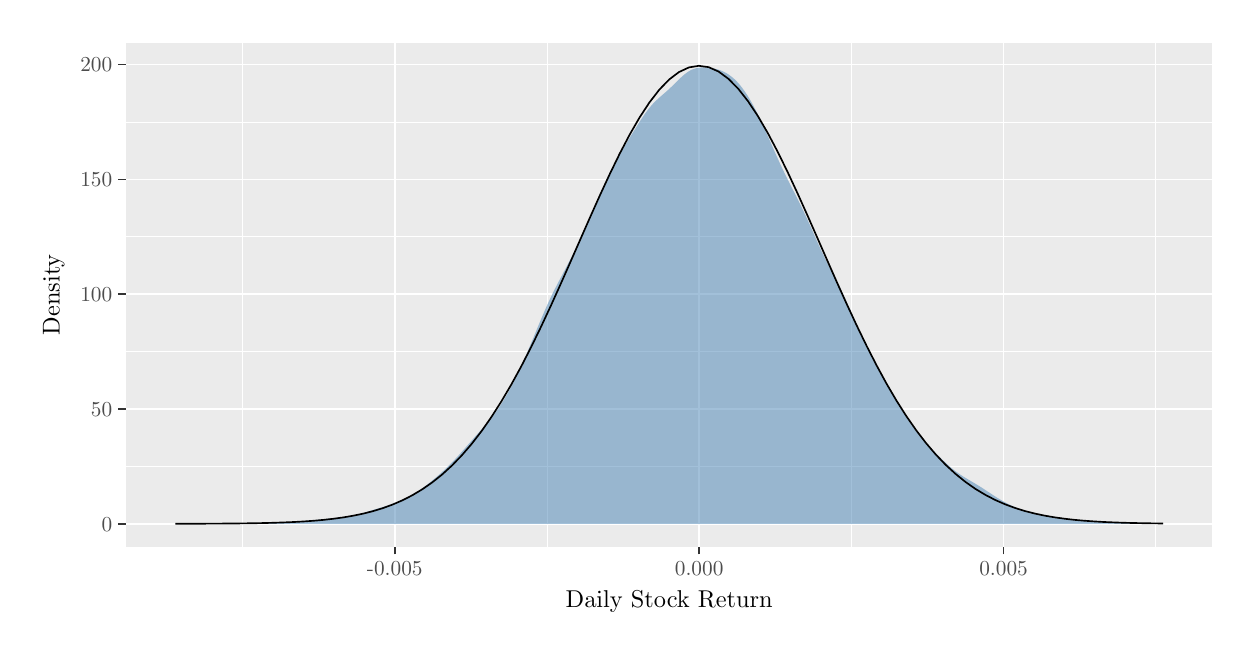
\begin{tikzpicture}[x=1pt,y=1pt]
\definecolor{fillColor}{RGB}{255,255,255}
\path[use as bounding box,fill=fillColor,fill opacity=0.00] (0,0) rectangle (433.62,216.81);
\begin{scope}
\path[clip] (  0.00,  0.00) rectangle (433.62,216.81);
\definecolor{drawColor}{RGB}{255,255,255}
\definecolor{fillColor}{RGB}{255,255,255}

\path[draw=drawColor,line width= 0.6pt,line join=round,line cap=round,fill=fillColor] (  0.00,  0.00) rectangle (433.62,216.81);
\end{scope}
\begin{scope}
\path[clip] ( 35.50, 29.26) rectangle (428.12,211.31);
\definecolor{fillColor}{gray}{0.92}

\path[fill=fillColor] ( 35.50, 29.26) rectangle (428.12,211.31);
\definecolor{drawColor}{RGB}{255,255,255}

\path[draw=drawColor,line width= 0.3pt,line join=round] ( 35.50, 58.28) --
	(428.12, 58.28);

\path[draw=drawColor,line width= 0.3pt,line join=round] ( 35.50, 99.76) --
	(428.12, 99.76);

\path[draw=drawColor,line width= 0.3pt,line join=round] ( 35.50,141.25) --
	(428.12,141.25);

\path[draw=drawColor,line width= 0.3pt,line join=round] ( 35.50,182.73) --
	(428.12,182.73);

\path[draw=drawColor,line width= 0.3pt,line join=round] ( 77.67, 29.26) --
	( 77.67,211.31);

\path[draw=drawColor,line width= 0.3pt,line join=round] (187.65, 29.26) --
	(187.65,211.31);

\path[draw=drawColor,line width= 0.3pt,line join=round] (297.64, 29.26) --
	(297.64,211.31);

\path[draw=drawColor,line width= 0.3pt,line join=round] (407.62, 29.26) --
	(407.62,211.31);

\path[draw=drawColor,line width= 0.6pt,line join=round] ( 35.50, 37.53) --
	(428.12, 37.53);

\path[draw=drawColor,line width= 0.6pt,line join=round] ( 35.50, 79.02) --
	(428.12, 79.02);

\path[draw=drawColor,line width= 0.6pt,line join=round] ( 35.50,120.50) --
	(428.12,120.50);

\path[draw=drawColor,line width= 0.6pt,line join=round] ( 35.50,161.99) --
	(428.12,161.99);

\path[draw=drawColor,line width= 0.6pt,line join=round] ( 35.50,203.47) --
	(428.12,203.47);

\path[draw=drawColor,line width= 0.6pt,line join=round] (132.66, 29.26) --
	(132.66,211.31);

\path[draw=drawColor,line width= 0.6pt,line join=round] (242.64, 29.26) --
	(242.64,211.31);

\path[draw=drawColor,line width= 0.6pt,line join=round] (352.63, 29.26) --
	(352.63,211.31);
\definecolor{fillColor}{RGB}{70,130,180}

\path[fill=fillColor,fill opacity=0.50] ( 53.35, 37.57) --
	( 54.05, 37.57) --
	( 54.75, 37.57) --
	( 55.44, 37.57) --
	( 56.14, 37.57) --
	( 56.84, 37.56) --
	( 57.54, 37.56) --
	( 58.24, 37.56) --
	( 58.94, 37.55) --
	( 59.63, 37.55) --
	( 60.33, 37.55) --
	( 61.03, 37.54) --
	( 61.73, 37.54) --
	( 62.43, 37.54) --
	( 63.13, 37.54) --
	( 63.83, 37.54) --
	( 64.52, 37.54) --
	( 65.22, 37.54) --
	( 65.92, 37.54) --
	( 66.62, 37.55) --
	( 67.32, 37.55) --
	( 68.02, 37.56) --
	( 68.71, 37.56) --
	( 69.41, 37.57) --
	( 70.11, 37.58) --
	( 70.81, 37.58) --
	( 71.51, 37.59) --
	( 72.21, 37.61) --
	( 72.91, 37.62) --
	( 73.60, 37.63) --
	( 74.30, 37.64) --
	( 75.00, 37.66) --
	( 75.70, 37.67) --
	( 76.40, 37.69) --
	( 77.10, 37.70) --
	( 77.80, 37.71) --
	( 78.49, 37.73) --
	( 79.19, 37.74) --
	( 79.89, 37.75) --
	( 80.59, 37.76) --
	( 81.29, 37.77) --
	( 81.99, 37.78) --
	( 82.68, 37.78) --
	( 83.38, 37.79) --
	( 84.08, 37.80) --
	( 84.78, 37.81) --
	( 85.48, 37.81) --
	( 86.18, 37.82) --
	( 86.88, 37.83) --
	( 87.57, 37.85) --
	( 88.27, 37.86) --
	( 88.97, 37.88) --
	( 89.67, 37.90) --
	( 90.37, 37.92) --
	( 91.07, 37.94) --
	( 91.76, 37.97) --
	( 92.46, 38.00) --
	( 93.16, 38.03) --
	( 93.86, 38.07) --
	( 94.56, 38.10) --
	( 95.26, 38.15) --
	( 95.96, 38.19) --
	( 96.65, 38.24) --
	( 97.35, 38.29) --
	( 98.05, 38.34) --
	( 98.75, 38.40) --
	( 99.45, 38.46) --
	(100.15, 38.52) --
	(100.85, 38.58) --
	(101.54, 38.64) --
	(102.24, 38.71) --
	(102.94, 38.77) --
	(103.64, 38.84) --
	(104.34, 38.91) --
	(105.04, 38.99) --
	(105.73, 39.06) --
	(106.43, 39.14) --
	(107.13, 39.22) --
	(107.83, 39.30) --
	(108.53, 39.38) --
	(109.23, 39.45) --
	(109.93, 39.53) --
	(110.62, 39.60) --
	(111.32, 39.67) --
	(112.02, 39.74) --
	(112.72, 39.81) --
	(113.42, 39.88) --
	(114.12, 39.95) --
	(114.81, 40.03) --
	(115.51, 40.12) --
	(116.21, 40.22) --
	(116.91, 40.33) --
	(117.61, 40.47) --
	(118.31, 40.61) --
	(119.01, 40.77) --
	(119.70, 40.95) --
	(120.40, 41.15) --
	(121.10, 41.35) --
	(121.80, 41.56) --
	(122.50, 41.78) --
	(123.20, 42.01) --
	(123.90, 42.23) --
	(124.59, 42.45) --
	(125.29, 42.67) --
	(125.99, 42.89) --
	(126.69, 43.10) --
	(127.39, 43.31) --
	(128.09, 43.51) --
	(128.78, 43.71) --
	(129.48, 43.92) --
	(130.18, 44.13) --
	(130.88, 44.35) --
	(131.58, 44.57) --
	(132.28, 44.81) --
	(132.98, 45.06) --
	(133.67, 45.33) --
	(134.37, 45.61) --
	(135.07, 45.91) --
	(135.77, 46.22) --
	(136.47, 46.56) --
	(137.17, 46.91) --
	(137.86, 47.29) --
	(138.56, 47.69) --
	(139.26, 48.11) --
	(139.96, 48.54) --
	(140.66, 49.00) --
	(141.36, 49.48) --
	(142.06, 49.97) --
	(142.75, 50.48) --
	(143.45, 51.00) --
	(144.15, 51.53) --
	(144.85, 52.08) --
	(145.55, 52.64) --
	(146.25, 53.21) --
	(146.95, 53.78) --
	(147.64, 54.37) --
	(148.34, 54.98) --
	(149.04, 55.59) --
	(149.74, 56.22) --
	(150.44, 56.86) --
	(151.14, 57.52) --
	(151.83, 58.20) --
	(152.53, 58.89) --
	(153.23, 59.60) --
	(153.93, 60.33) --
	(154.63, 61.08) --
	(155.33, 61.83) --
	(156.03, 62.60) --
	(156.72, 63.38) --
	(157.42, 64.17) --
	(158.12, 64.96) --
	(158.82, 65.76) --
	(159.52, 66.56) --
	(160.22, 67.36) --
	(160.91, 68.15) --
	(161.61, 68.95) --
	(162.31, 69.74) --
	(163.01, 70.52) --
	(163.71, 71.31) --
	(164.41, 72.10) --
	(165.11, 72.90) --
	(165.80, 73.70) --
	(166.50, 74.52) --
	(167.20, 75.37) --
	(167.90, 76.25) --
	(168.60, 77.16) --
	(169.30, 78.11) --
	(170.00, 79.10) --
	(170.69, 80.15) --
	(171.39, 81.24) --
	(172.09, 82.37) --
	(172.79, 83.56) --
	(173.49, 84.80) --
	(174.19, 86.09) --
	(174.88, 87.42) --
	(175.58, 88.80) --
	(176.28, 90.21) --
	(176.98, 91.66) --
	(177.68, 93.15) --
	(178.38, 94.66) --
	(179.08, 96.21) --
	(179.77, 97.79) --
	(180.47, 99.40) --
	(181.17,101.03) --
	(181.87,102.68) --
	(182.57,104.35) --
	(183.27,106.04) --
	(183.96,107.73) --
	(184.66,109.42) --
	(185.36,111.10) --
	(186.06,112.75) --
	(186.76,114.38) --
	(187.46,115.97) --
	(188.16,117.52) --
	(188.85,119.02) --
	(189.55,120.48) --
	(190.25,121.89) --
	(190.95,123.27) --
	(191.65,124.62) --
	(192.35,125.95) --
	(193.05,127.27) --
	(193.74,128.59) --
	(194.44,129.92) --
	(195.14,131.25) --
	(195.84,132.60) --
	(196.54,133.96) --
	(197.24,135.35) --
	(197.93,136.75) --
	(198.63,138.18) --
	(199.33,139.62) --
	(200.03,141.09) --
	(200.73,142.59) --
	(201.43,144.11) --
	(202.13,145.65) --
	(202.82,147.23) --
	(203.52,148.83) --
	(204.22,150.45) --
	(204.92,152.09) --
	(205.62,153.74) --
	(206.32,155.38) --
	(207.01,157.02) --
	(207.71,158.63) --
	(208.41,160.22) --
	(209.11,161.76) --
	(209.81,163.27) --
	(210.51,164.72) --
	(211.21,166.11) --
	(211.90,167.46) --
	(212.60,168.75) --
	(213.30,170.00) --
	(214.00,171.22) --
	(214.70,172.40) --
	(215.40,173.56) --
	(216.10,174.70) --
	(216.79,175.84) --
	(217.49,176.97) --
	(218.19,178.10) --
	(218.89,179.22) --
	(219.59,180.35) --
	(220.29,181.47) --
	(220.98,182.57) --
	(221.68,183.65) --
	(222.38,184.71) --
	(223.08,185.72) --
	(223.78,186.69) --
	(224.48,187.60) --
	(225.18,188.44) --
	(225.87,189.23) --
	(226.57,189.96) --
	(227.27,190.64) --
	(227.97,191.29) --
	(228.67,191.90) --
	(229.37,192.51) --
	(230.06,193.11) --
	(230.76,193.72) --
	(231.46,194.34) --
	(232.16,194.99) --
	(232.86,195.66) --
	(233.56,196.34) --
	(234.26,197.04) --
	(234.95,197.73) --
	(235.65,198.41) --
	(236.35,199.06) --
	(237.05,199.67) --
	(237.75,200.24) --
	(238.45,200.75) --
	(239.15,201.19) --
	(239.84,201.56) --
	(240.54,201.85) --
	(241.24,202.08) --
	(241.94,202.25) --
	(242.64,202.36) --
	(243.34,202.42) --
	(244.03,202.44) --
	(244.73,202.43) --
	(245.43,202.39) --
	(246.13,202.32) --
	(246.83,202.24) --
	(247.53,202.12) --
	(248.23,201.99) --
	(248.92,201.82) --
	(249.62,201.62) --
	(250.32,201.38) --
	(251.02,201.11) --
	(251.72,200.78) --
	(252.42,200.41) --
	(253.11,199.99) --
	(253.81,199.50) --
	(254.51,198.96) --
	(255.21,198.36) --
	(255.91,197.69) --
	(256.61,196.96) --
	(257.31,196.16) --
	(258.00,195.29) --
	(258.70,194.35) --
	(259.40,193.35) --
	(260.10,192.28) --
	(260.80,191.14) --
	(261.50,189.94) --
	(262.20,188.68) --
	(262.89,187.36) --
	(263.59,185.99) --
	(264.29,184.57) --
	(264.99,183.10) --
	(265.69,181.60) --
	(266.39,180.05) --
	(267.08,178.49) --
	(267.78,176.90) --
	(268.48,175.30) --
	(269.18,173.70) --
	(269.88,172.11) --
	(270.58,170.53) --
	(271.28,168.98) --
	(271.97,167.45) --
	(272.67,165.96) --
	(273.37,164.50) --
	(274.07,163.07) --
	(274.77,161.66) --
	(275.47,160.27) --
	(276.16,158.90) --
	(276.86,157.53) --
	(277.56,156.16) --
	(278.26,154.77) --
	(278.96,153.37) --
	(279.66,151.94) --
	(280.36,150.48) --
	(281.05,148.99) --
	(281.75,147.47) --
	(282.45,145.93) --
	(283.15,144.36) --
	(283.85,142.78) --
	(284.55,141.20) --
	(285.25,139.62) --
	(285.94,138.07) --
	(286.64,136.55) --
	(287.34,135.06) --
	(288.04,133.61) --
	(288.74,132.19) --
	(289.44,130.81) --
	(290.13,129.45) --
	(290.83,128.11) --
	(291.53,126.76) --
	(292.23,125.41) --
	(292.93,124.03) --
	(293.63,122.63) --
	(294.33,121.18) --
	(295.02,119.70) --
	(295.72,118.17) --
	(296.42,116.62) --
	(297.12,115.03) --
	(297.82,113.42) --
	(298.52,111.80) --
	(299.21,110.18) --
	(299.91,108.58) --
	(300.61,106.99) --
	(301.31,105.43) --
	(302.01,103.90) --
	(302.71,102.40) --
	(303.41,100.94) --
	(304.10, 99.52) --
	(304.80, 98.13) --
	(305.50, 96.78) --
	(306.20, 95.46) --
	(306.90, 94.17) --
	(307.60, 92.90) --
	(308.30, 91.65) --
	(308.99, 90.41) --
	(309.69, 89.19) --
	(310.39, 87.98) --
	(311.09, 86.78) --
	(311.79, 85.58) --
	(312.49, 84.39) --
	(313.18, 83.20) --
	(313.88, 82.01) --
	(314.58, 80.84) --
	(315.28, 79.67) --
	(315.98, 78.52) --
	(316.68, 77.38) --
	(317.38, 76.26) --
	(318.07, 75.18) --
	(318.77, 74.12) --
	(319.47, 73.10) --
	(320.17, 72.12) --
	(320.87, 71.18) --
	(321.57, 70.28) --
	(322.26, 69.41) --
	(322.96, 68.58) --
	(323.66, 67.78) --
	(324.36, 67.01) --
	(325.06, 66.25) --
	(325.76, 65.51) --
	(326.46, 64.79) --
	(327.15, 64.07) --
	(327.85, 63.36) --
	(328.55, 62.66) --
	(329.25, 61.96) --
	(329.95, 61.27) --
	(330.65, 60.58) --
	(331.35, 59.91) --
	(332.04, 59.26) --
	(332.74, 58.62) --
	(333.44, 58.01) --
	(334.14, 57.42) --
	(334.84, 56.86) --
	(335.54, 56.33) --
	(336.23, 55.83) --
	(336.93, 55.35) --
	(337.63, 54.89) --
	(338.33, 54.46) --
	(339.03, 54.03) --
	(339.73, 53.62) --
	(340.43, 53.21) --
	(341.12, 52.80) --
	(341.82, 52.39) --
	(342.52, 51.97) --
	(343.22, 51.55) --
	(343.92, 51.12) --
	(344.62, 50.68) --
	(345.31, 50.23) --
	(346.01, 49.77) --
	(346.71, 49.31) --
	(347.41, 48.85) --
	(348.11, 48.39) --
	(348.81, 47.93) --
	(349.51, 47.48) --
	(350.20, 47.04) --
	(350.90, 46.60) --
	(351.60, 46.18) --
	(352.30, 45.78) --
	(353.00, 45.38) --
	(353.70, 45.01) --
	(354.39, 44.65) --
	(355.09, 44.31) --
	(355.79, 43.98) --
	(356.49, 43.67) --
	(357.19, 43.37) --
	(357.89, 43.09) --
	(358.59, 42.82) --
	(359.28, 42.56) --
	(359.98, 42.32) --
	(360.68, 42.10) --
	(361.38, 41.88) --
	(362.08, 41.68) --
	(362.78, 41.50) --
	(363.48, 41.32) --
	(364.17, 41.16) --
	(364.87, 41.01) --
	(365.57, 40.86) --
	(366.27, 40.73) --
	(366.97, 40.60) --
	(367.67, 40.48) --
	(368.36, 40.36) --
	(369.06, 40.25) --
	(369.76, 40.15) --
	(370.46, 40.05) --
	(371.16, 39.95) --
	(371.86, 39.85) --
	(372.56, 39.76) --
	(373.25, 39.67) --
	(373.95, 39.58) --
	(374.65, 39.49) --
	(375.35, 39.40) --
	(376.05, 39.32) --
	(376.75, 39.23) --
	(377.44, 39.15) --
	(378.14, 39.06) --
	(378.84, 38.98) --
	(379.54, 38.90) --
	(380.24, 38.82) --
	(380.94, 38.74) --
	(381.64, 38.66) --
	(382.33, 38.59) --
	(383.03, 38.53) --
	(383.73, 38.46) --
	(384.43, 38.40) --
	(385.13, 38.35) --
	(385.83, 38.29) --
	(386.53, 38.25) --
	(387.22, 38.20) --
	(387.92, 38.16) --
	(388.62, 38.12) --
	(389.32, 38.08) --
	(390.02, 38.04) --
	(390.72, 38.01) --
	(391.41, 37.98) --
	(392.11, 37.95) --
	(392.81, 37.93) --
	(393.51, 37.90) --
	(394.21, 37.89) --
	(394.91, 37.87) --
	(395.61, 37.86) --
	(396.30, 37.85) --
	(397.00, 37.84) --
	(397.70, 37.84) --
	(398.40, 37.83) --
	(399.10, 37.83) --
	(399.80, 37.83) --
	(400.49, 37.83) --
	(401.19, 37.83) --
	(401.89, 37.83) --
	(402.59, 37.82) --
	(403.29, 37.82) --
	(403.99, 37.81) --
	(404.69, 37.80) --
	(405.38, 37.79) --
	(406.08, 37.78) --
	(406.78, 37.76) --
	(407.48, 37.75) --
	(408.18, 37.73) --
	(408.88, 37.72) --
	(409.58, 37.70) --
	(410.27, 37.69) --
	(410.27, 37.53) --
	(409.58, 37.53) --
	(408.88, 37.53) --
	(408.18, 37.53) --
	(407.48, 37.53) --
	(406.78, 37.53) --
	(406.08, 37.53) --
	(405.38, 37.53) --
	(404.69, 37.53) --
	(403.99, 37.53) --
	(403.29, 37.53) --
	(402.59, 37.53) --
	(401.89, 37.53) --
	(401.19, 37.53) --
	(400.49, 37.53) --
	(399.80, 37.53) --
	(399.10, 37.53) --
	(398.40, 37.53) --
	(397.70, 37.53) --
	(397.00, 37.53) --
	(396.30, 37.53) --
	(395.61, 37.53) --
	(394.91, 37.53) --
	(394.21, 37.53) --
	(393.51, 37.53) --
	(392.81, 37.53) --
	(392.11, 37.53) --
	(391.41, 37.53) --
	(390.72, 37.53) --
	(390.02, 37.53) --
	(389.32, 37.53) --
	(388.62, 37.53) --
	(387.92, 37.53) --
	(387.22, 37.53) --
	(386.53, 37.53) --
	(385.83, 37.53) --
	(385.13, 37.53) --
	(384.43, 37.53) --
	(383.73, 37.53) --
	(383.03, 37.53) --
	(382.33, 37.53) --
	(381.64, 37.53) --
	(380.94, 37.53) --
	(380.24, 37.53) --
	(379.54, 37.53) --
	(378.84, 37.53) --
	(378.14, 37.53) --
	(377.44, 37.53) --
	(376.75, 37.53) --
	(376.05, 37.53) --
	(375.35, 37.53) --
	(374.65, 37.53) --
	(373.95, 37.53) --
	(373.25, 37.53) --
	(372.56, 37.53) --
	(371.86, 37.53) --
	(371.16, 37.53) --
	(370.46, 37.53) --
	(369.76, 37.53) --
	(369.06, 37.53) --
	(368.36, 37.53) --
	(367.67, 37.53) --
	(366.97, 37.53) --
	(366.27, 37.53) --
	(365.57, 37.53) --
	(364.87, 37.53) --
	(364.17, 37.53) --
	(363.48, 37.53) --
	(362.78, 37.53) --
	(362.08, 37.53) --
	(361.38, 37.53) --
	(360.68, 37.53) --
	(359.98, 37.53) --
	(359.28, 37.53) --
	(358.59, 37.53) --
	(357.89, 37.53) --
	(357.19, 37.53) --
	(356.49, 37.53) --
	(355.79, 37.53) --
	(355.09, 37.53) --
	(354.39, 37.53) --
	(353.70, 37.53) --
	(353.00, 37.53) --
	(352.30, 37.53) --
	(351.60, 37.53) --
	(350.90, 37.53) --
	(350.20, 37.53) --
	(349.51, 37.53) --
	(348.81, 37.53) --
	(348.11, 37.53) --
	(347.41, 37.53) --
	(346.71, 37.53) --
	(346.01, 37.53) --
	(345.31, 37.53) --
	(344.62, 37.53) --
	(343.92, 37.53) --
	(343.22, 37.53) --
	(342.52, 37.53) --
	(341.82, 37.53) --
	(341.12, 37.53) --
	(340.43, 37.53) --
	(339.73, 37.53) --
	(339.03, 37.53) --
	(338.33, 37.53) --
	(337.63, 37.53) --
	(336.93, 37.53) --
	(336.23, 37.53) --
	(335.54, 37.53) --
	(334.84, 37.53) --
	(334.14, 37.53) --
	(333.44, 37.53) --
	(332.74, 37.53) --
	(332.04, 37.53) --
	(331.35, 37.53) --
	(330.65, 37.53) --
	(329.95, 37.53) --
	(329.25, 37.53) --
	(328.55, 37.53) --
	(327.85, 37.53) --
	(327.15, 37.53) --
	(326.46, 37.53) --
	(325.76, 37.53) --
	(325.06, 37.53) --
	(324.36, 37.53) --
	(323.66, 37.53) --
	(322.96, 37.53) --
	(322.26, 37.53) --
	(321.57, 37.53) --
	(320.87, 37.53) --
	(320.17, 37.53) --
	(319.47, 37.53) --
	(318.77, 37.53) --
	(318.07, 37.53) --
	(317.38, 37.53) --
	(316.68, 37.53) --
	(315.98, 37.53) --
	(315.28, 37.53) --
	(314.58, 37.53) --
	(313.88, 37.53) --
	(313.18, 37.53) --
	(312.49, 37.53) --
	(311.79, 37.53) --
	(311.09, 37.53) --
	(310.39, 37.53) --
	(309.69, 37.53) --
	(308.99, 37.53) --
	(308.30, 37.53) --
	(307.60, 37.53) --
	(306.90, 37.53) --
	(306.20, 37.53) --
	(305.50, 37.53) --
	(304.80, 37.53) --
	(304.10, 37.53) --
	(303.41, 37.53) --
	(302.71, 37.53) --
	(302.01, 37.53) --
	(301.31, 37.53) --
	(300.61, 37.53) --
	(299.91, 37.53) --
	(299.21, 37.53) --
	(298.52, 37.53) --
	(297.82, 37.53) --
	(297.12, 37.53) --
	(296.42, 37.53) --
	(295.72, 37.53) --
	(295.02, 37.53) --
	(294.33, 37.53) --
	(293.63, 37.53) --
	(292.93, 37.53) --
	(292.23, 37.53) --
	(291.53, 37.53) --
	(290.83, 37.53) --
	(290.13, 37.53) --
	(289.44, 37.53) --
	(288.74, 37.53) --
	(288.04, 37.53) --
	(287.34, 37.53) --
	(286.64, 37.53) --
	(285.94, 37.53) --
	(285.25, 37.53) --
	(284.55, 37.53) --
	(283.85, 37.53) --
	(283.15, 37.53) --
	(282.45, 37.53) --
	(281.75, 37.53) --
	(281.05, 37.53) --
	(280.36, 37.53) --
	(279.66, 37.53) --
	(278.96, 37.53) --
	(278.26, 37.53) --
	(277.56, 37.53) --
	(276.86, 37.53) --
	(276.16, 37.53) --
	(275.47, 37.53) --
	(274.77, 37.53) --
	(274.07, 37.53) --
	(273.37, 37.53) --
	(272.67, 37.53) --
	(271.97, 37.53) --
	(271.28, 37.53) --
	(270.58, 37.53) --
	(269.88, 37.53) --
	(269.18, 37.53) --
	(268.48, 37.53) --
	(267.78, 37.53) --
	(267.08, 37.53) --
	(266.39, 37.53) --
	(265.69, 37.53) --
	(264.99, 37.53) --
	(264.29, 37.53) --
	(263.59, 37.53) --
	(262.89, 37.53) --
	(262.20, 37.53) --
	(261.50, 37.53) --
	(260.80, 37.53) --
	(260.10, 37.53) --
	(259.40, 37.53) --
	(258.70, 37.53) --
	(258.00, 37.53) --
	(257.31, 37.53) --
	(256.61, 37.53) --
	(255.91, 37.53) --
	(255.21, 37.53) --
	(254.51, 37.53) --
	(253.81, 37.53) --
	(253.11, 37.53) --
	(252.42, 37.53) --
	(251.72, 37.53) --
	(251.02, 37.53) --
	(250.32, 37.53) --
	(249.62, 37.53) --
	(248.92, 37.53) --
	(248.23, 37.53) --
	(247.53, 37.53) --
	(246.83, 37.53) --
	(246.13, 37.53) --
	(245.43, 37.53) --
	(244.73, 37.53) --
	(244.03, 37.53) --
	(243.34, 37.53) --
	(242.64, 37.53) --
	(241.94, 37.53) --
	(241.24, 37.53) --
	(240.54, 37.53) --
	(239.84, 37.53) --
	(239.15, 37.53) --
	(238.45, 37.53) --
	(237.75, 37.53) --
	(237.05, 37.53) --
	(236.35, 37.53) --
	(235.65, 37.53) --
	(234.95, 37.53) --
	(234.26, 37.53) --
	(233.56, 37.53) --
	(232.86, 37.53) --
	(232.16, 37.53) --
	(231.46, 37.53) --
	(230.76, 37.53) --
	(230.06, 37.53) --
	(229.37, 37.53) --
	(228.67, 37.53) --
	(227.97, 37.53) --
	(227.27, 37.53) --
	(226.57, 37.53) --
	(225.87, 37.53) --
	(225.18, 37.53) --
	(224.48, 37.53) --
	(223.78, 37.53) --
	(223.08, 37.53) --
	(222.38, 37.53) --
	(221.68, 37.53) --
	(220.98, 37.53) --
	(220.29, 37.53) --
	(219.59, 37.53) --
	(218.89, 37.53) --
	(218.19, 37.53) --
	(217.49, 37.53) --
	(216.79, 37.53) --
	(216.10, 37.53) --
	(215.40, 37.53) --
	(214.70, 37.53) --
	(214.00, 37.53) --
	(213.30, 37.53) --
	(212.60, 37.53) --
	(211.90, 37.53) --
	(211.21, 37.53) --
	(210.51, 37.53) --
	(209.81, 37.53) --
	(209.11, 37.53) --
	(208.41, 37.53) --
	(207.71, 37.53) --
	(207.01, 37.53) --
	(206.32, 37.53) --
	(205.62, 37.53) --
	(204.92, 37.53) --
	(204.22, 37.53) --
	(203.52, 37.53) --
	(202.82, 37.53) --
	(202.13, 37.53) --
	(201.43, 37.53) --
	(200.73, 37.53) --
	(200.03, 37.53) --
	(199.33, 37.53) --
	(198.63, 37.53) --
	(197.93, 37.53) --
	(197.24, 37.53) --
	(196.54, 37.53) --
	(195.84, 37.53) --
	(195.14, 37.53) --
	(194.44, 37.53) --
	(193.74, 37.53) --
	(193.05, 37.53) --
	(192.35, 37.53) --
	(191.65, 37.53) --
	(190.95, 37.53) --
	(190.25, 37.53) --
	(189.55, 37.53) --
	(188.85, 37.53) --
	(188.16, 37.53) --
	(187.46, 37.53) --
	(186.76, 37.53) --
	(186.06, 37.53) --
	(185.36, 37.53) --
	(184.66, 37.53) --
	(183.96, 37.53) --
	(183.27, 37.53) --
	(182.57, 37.53) --
	(181.87, 37.53) --
	(181.17, 37.53) --
	(180.47, 37.53) --
	(179.77, 37.53) --
	(179.08, 37.53) --
	(178.38, 37.53) --
	(177.68, 37.53) --
	(176.98, 37.53) --
	(176.28, 37.53) --
	(175.58, 37.53) --
	(174.88, 37.53) --
	(174.19, 37.53) --
	(173.49, 37.53) --
	(172.79, 37.53) --
	(172.09, 37.53) --
	(171.39, 37.53) --
	(170.69, 37.53) --
	(170.00, 37.53) --
	(169.30, 37.53) --
	(168.60, 37.53) --
	(167.90, 37.53) --
	(167.20, 37.53) --
	(166.50, 37.53) --
	(165.80, 37.53) --
	(165.11, 37.53) --
	(164.41, 37.53) --
	(163.71, 37.53) --
	(163.01, 37.53) --
	(162.31, 37.53) --
	(161.61, 37.53) --
	(160.91, 37.53) --
	(160.22, 37.53) --
	(159.52, 37.53) --
	(158.82, 37.53) --
	(158.12, 37.53) --
	(157.42, 37.53) --
	(156.72, 37.53) --
	(156.03, 37.53) --
	(155.33, 37.53) --
	(154.63, 37.53) --
	(153.93, 37.53) --
	(153.23, 37.53) --
	(152.53, 37.53) --
	(151.83, 37.53) --
	(151.14, 37.53) --
	(150.44, 37.53) --
	(149.74, 37.53) --
	(149.04, 37.53) --
	(148.34, 37.53) --
	(147.64, 37.53) --
	(146.95, 37.53) --
	(146.25, 37.53) --
	(145.55, 37.53) --
	(144.85, 37.53) --
	(144.15, 37.53) --
	(143.45, 37.53) --
	(142.75, 37.53) --
	(142.06, 37.53) --
	(141.36, 37.53) --
	(140.66, 37.53) --
	(139.96, 37.53) --
	(139.26, 37.53) --
	(138.56, 37.53) --
	(137.86, 37.53) --
	(137.17, 37.53) --
	(136.47, 37.53) --
	(135.77, 37.53) --
	(135.07, 37.53) --
	(134.37, 37.53) --
	(133.67, 37.53) --
	(132.98, 37.53) --
	(132.28, 37.53) --
	(131.58, 37.53) --
	(130.88, 37.53) --
	(130.18, 37.53) --
	(129.48, 37.53) --
	(128.78, 37.53) --
	(128.09, 37.53) --
	(127.39, 37.53) --
	(126.69, 37.53) --
	(125.99, 37.53) --
	(125.29, 37.53) --
	(124.59, 37.53) --
	(123.90, 37.53) --
	(123.20, 37.53) --
	(122.50, 37.53) --
	(121.80, 37.53) --
	(121.10, 37.53) --
	(120.40, 37.53) --
	(119.70, 37.53) --
	(119.01, 37.53) --
	(118.31, 37.53) --
	(117.61, 37.53) --
	(116.91, 37.53) --
	(116.21, 37.53) --
	(115.51, 37.53) --
	(114.81, 37.53) --
	(114.12, 37.53) --
	(113.42, 37.53) --
	(112.72, 37.53) --
	(112.02, 37.53) --
	(111.32, 37.53) --
	(110.62, 37.53) --
	(109.93, 37.53) --
	(109.23, 37.53) --
	(108.53, 37.53) --
	(107.83, 37.53) --
	(107.13, 37.53) --
	(106.43, 37.53) --
	(105.73, 37.53) --
	(105.04, 37.53) --
	(104.34, 37.53) --
	(103.64, 37.53) --
	(102.94, 37.53) --
	(102.24, 37.53) --
	(101.54, 37.53) --
	(100.85, 37.53) --
	(100.15, 37.53) --
	( 99.45, 37.53) --
	( 98.75, 37.53) --
	( 98.05, 37.53) --
	( 97.35, 37.53) --
	( 96.65, 37.53) --
	( 95.96, 37.53) --
	( 95.26, 37.53) --
	( 94.56, 37.53) --
	( 93.86, 37.53) --
	( 93.16, 37.53) --
	( 92.46, 37.53) --
	( 91.76, 37.53) --
	( 91.07, 37.53) --
	( 90.37, 37.53) --
	( 89.67, 37.53) --
	( 88.97, 37.53) --
	( 88.27, 37.53) --
	( 87.57, 37.53) --
	( 86.88, 37.53) --
	( 86.18, 37.53) --
	( 85.48, 37.53) --
	( 84.78, 37.53) --
	( 84.08, 37.53) --
	( 83.38, 37.53) --
	( 82.68, 37.53) --
	( 81.99, 37.53) --
	( 81.29, 37.53) --
	( 80.59, 37.53) --
	( 79.89, 37.53) --
	( 79.19, 37.53) --
	( 78.49, 37.53) --
	( 77.80, 37.53) --
	( 77.10, 37.53) --
	( 76.40, 37.53) --
	( 75.70, 37.53) --
	( 75.00, 37.53) --
	( 74.30, 37.53) --
	( 73.60, 37.53) --
	( 72.91, 37.53) --
	( 72.21, 37.53) --
	( 71.51, 37.53) --
	( 70.81, 37.53) --
	( 70.11, 37.53) --
	( 69.41, 37.53) --
	( 68.71, 37.53) --
	( 68.02, 37.53) --
	( 67.32, 37.53) --
	( 66.62, 37.53) --
	( 65.92, 37.53) --
	( 65.22, 37.53) --
	( 64.52, 37.53) --
	( 63.83, 37.53) --
	( 63.13, 37.53) --
	( 62.43, 37.53) --
	( 61.73, 37.53) --
	( 61.03, 37.53) --
	( 60.33, 37.53) --
	( 59.63, 37.53) --
	( 58.94, 37.53) --
	( 58.24, 37.53) --
	( 57.54, 37.53) --
	( 56.84, 37.53) --
	( 56.14, 37.53) --
	( 55.44, 37.53) --
	( 54.75, 37.53) --
	( 54.05, 37.53) --
	( 53.35, 37.53) --
	cycle;
\definecolor{drawColor}{RGB}{0,0,0}

\path[draw=drawColor,line width= 0.6pt,line join=round] ( 53.35, 37.55) --
	( 56.92, 37.56) --
	( 60.49, 37.56) --
	( 64.06, 37.58) --
	( 67.63, 37.59) --
	( 71.19, 37.62) --
	( 74.76, 37.65) --
	( 78.33, 37.69) --
	( 81.90, 37.74) --
	( 85.47, 37.81) --
	( 89.04, 37.91) --
	( 92.61, 38.03) --
	( 96.18, 38.18) --
	( 99.75, 38.38) --
	(103.32, 38.63) --
	(106.89, 38.95) --
	(110.46, 39.35) --
	(114.03, 39.84) --
	(117.59, 40.45) --
	(121.16, 41.19) --
	(124.73, 42.09) --
	(128.30, 43.18) --
	(131.87, 44.49) --
	(135.44, 46.03) --
	(139.01, 47.86) --
	(142.58, 49.99) --
	(146.15, 52.47) --
	(149.72, 55.31) --
	(153.29, 58.57) --
	(156.86, 62.26) --
	(160.43, 66.40) --
	(164.00, 71.01) --
	(167.56, 76.11) --
	(171.13, 81.70) --
	(174.70, 87.76) --
	(178.27, 94.27) --
	(181.84,101.22) --
	(185.41,108.54) --
	(188.98,116.18) --
	(192.55,124.08) --
	(196.12,132.14) --
	(199.69,140.28) --
	(203.26,148.39) --
	(206.83,156.35) --
	(210.40,164.04) --
	(213.96,171.35) --
	(217.53,178.16) --
	(221.10,184.34) --
	(224.67,189.79) --
	(228.24,194.40) --
	(231.81,198.09) --
	(235.38,200.79) --
	(238.95,202.45) --
	(242.52,203.03) --
	(246.09,202.53) --
	(249.66,200.95) --
	(253.23,198.32) --
	(256.80,194.69) --
	(260.37,190.14) --
	(263.93,184.75) --
	(267.50,178.62) --
	(271.07,171.85) --
	(274.64,164.57) --
	(278.21,156.90) --
	(281.78,148.95) --
	(285.35,140.86) --
	(288.92,132.72) --
	(292.49,124.64) --
	(296.06,116.73) --
	(299.63,109.07) --
	(303.20,101.72) --
	(306.77, 94.75) --
	(310.33, 88.20) --
	(313.90, 82.11) --
	(317.47, 76.49) --
	(321.04, 71.36) --
	(324.61, 66.71) --
	(328.18, 62.53) --
	(331.75, 58.81) --
	(335.32, 55.53) --
	(338.89, 52.65) --
	(342.46, 50.15) --
	(346.03, 48.00) --
	(349.60, 46.15) --
	(353.17, 44.59) --
	(356.73, 43.27) --
	(360.30, 42.16) --
	(363.87, 41.25) --
	(367.44, 40.49) --
	(371.01, 39.88) --
	(374.58, 39.38) --
	(378.15, 38.97) --
	(381.72, 38.65) --
	(385.29, 38.40) --
	(388.86, 38.19) --
	(392.43, 38.04) --
	(396.00, 37.91) --
	(399.57, 37.82) --
	(403.14, 37.75) --
	(406.70, 37.69) --
	(410.27, 37.65);
\end{scope}
\begin{scope}
\path[clip] (  0.00,  0.00) rectangle (433.62,216.81);
\definecolor{drawColor}{gray}{0.30}

\node[text=drawColor,anchor=base east,inner sep=0pt, outer sep=0pt, scale=  0.77] at ( 30.55, 34.88) {0};

\node[text=drawColor,anchor=base east,inner sep=0pt, outer sep=0pt, scale=  0.77] at ( 30.55, 76.37) {50};

\node[text=drawColor,anchor=base east,inner sep=0pt, outer sep=0pt, scale=  0.77] at ( 30.55,117.85) {100};

\node[text=drawColor,anchor=base east,inner sep=0pt, outer sep=0pt, scale=  0.77] at ( 30.55,159.34) {150};

\node[text=drawColor,anchor=base east,inner sep=0pt, outer sep=0pt, scale=  0.77] at ( 30.55,200.82) {200};
\end{scope}
\begin{scope}
\path[clip] (  0.00,  0.00) rectangle (433.62,216.81);
\definecolor{drawColor}{gray}{0.20}

\path[draw=drawColor,line width= 0.6pt,line join=round] ( 32.75, 37.53) --
	( 35.50, 37.53);

\path[draw=drawColor,line width= 0.6pt,line join=round] ( 32.75, 79.02) --
	( 35.50, 79.02);

\path[draw=drawColor,line width= 0.6pt,line join=round] ( 32.75,120.50) --
	( 35.50,120.50);

\path[draw=drawColor,line width= 0.6pt,line join=round] ( 32.75,161.99) --
	( 35.50,161.99);

\path[draw=drawColor,line width= 0.6pt,line join=round] ( 32.75,203.47) --
	( 35.50,203.47);
\end{scope}
\begin{scope}
\path[clip] (  0.00,  0.00) rectangle (433.62,216.81);
\definecolor{drawColor}{gray}{0.20}

\path[draw=drawColor,line width= 0.6pt,line join=round] (132.66, 26.51) --
	(132.66, 29.26);

\path[draw=drawColor,line width= 0.6pt,line join=round] (242.64, 26.51) --
	(242.64, 29.26);

\path[draw=drawColor,line width= 0.6pt,line join=round] (352.63, 26.51) --
	(352.63, 29.26);
\end{scope}
\begin{scope}
\path[clip] (  0.00,  0.00) rectangle (433.62,216.81);
\definecolor{drawColor}{gray}{0.30}

\node[text=drawColor,anchor=base,inner sep=0pt, outer sep=0pt, scale=  0.77] at (132.66, 19.00) {-0.005};

\node[text=drawColor,anchor=base,inner sep=0pt, outer sep=0pt, scale=  0.77] at (242.64, 19.00) {0.000};

\node[text=drawColor,anchor=base,inner sep=0pt, outer sep=0pt, scale=  0.77] at (352.63, 19.00) {0.005};
\end{scope}
\begin{scope}
\path[clip] (  0.00,  0.00) rectangle (433.62,216.81);
\definecolor{drawColor}{RGB}{0,0,0}

\node[text=drawColor,anchor=base,inner sep=0pt, outer sep=0pt, scale=  0.88] at (231.81,  7.44) {Daily Stock Return};
\end{scope}
\begin{scope}
\path[clip] (  0.00,  0.00) rectangle (433.62,216.81);
\definecolor{drawColor}{RGB}{0,0,0}

\node[text=drawColor,rotate= 90.00,anchor=base,inner sep=0pt, outer sep=0pt, scale=  0.88] at ( 11.56,120.28) {Density};
\end{scope}
\end{tikzpicture}

\caption{Daily Basis Stock Return Density}
\label{plot:returnDensity}
\end{figure}

%%%%%%%%%%%%%%%%%%%%%%%%%%%%%%%%%%%%%%%%%%%%%%%%
% SUBSECTION: Distribution of the stock price process
%%%%%%%%%%%%%%%%%%%%%%%%%%%%%%%%%%%%%%%%%%%%%%%%
\subsection{Distribution of the stock price process}
\label{sub:Distribution of the stock price process}

According to Itô's approximation and by setting $\ft$ to be $\ln{\St}$ it is showed that the natural logarith of $\St$ is normaly distributed with mean
$\left(\alpha - \frac{\sigma^2}{2}\right) \Dt$ and variance $\sigma^2 \Dt$.
Because every process with normally distributed logarithm are log--normally distributed, and following the relationship between the two laws, $\St$ is consequently log--normally distributed with mean () and var ().

MEAN
VAR

%%%%%%%%%%%%%%%%%%%%%%%%%%%%%%%%%%%%%%%%%%%%%%%%
% SUBSECTION: Flaws
%%%%%%%%%%%%%%%%%%%%%%%%%%%%%%%%%%%%%%%%%%%%%%%%
\subsection{Flaws}
\label{sub:Flaws}



%%%%%%%%%%%%%%%%%%%%%%%%%%%%%%%%%%%%%%%%%%%%%%%%
% SECTION: Volatility issues
%%%%%%%%%%%%%%%%%%%%%%%%%%%%%%%%%%%%%%%%%%%%%%%%
\section{Volatility issues}
\label{sec:Volatility issues}



%%%%%%%%%%%%%%%%%%%%%%%%%%%%%%%%%%%%%%%%%%%%%%%%
% SECTION: Jump issues
%%%%%%%%%%%%%%%%%%%%%%%%%%%%%%%%%%%%%%%%%%%%%%%%
\section{Jump issues}
\label{sec:Jump issues}
%%%%%%%%%%%%%%%%%%%%%%%%%%%%%%%%%%%%%%%%%%%%%%%%%%%%%%%%%%%%%%%%%%%%%%%%%%%%%%%%
%
%  CHAPTER:The Greeks
%
%%%%%%%%%%%%%%%%%%%%%%%%%%%%%%%%%%%%%%%%%%%%%%%%%%%%%%%%%%%%%%%%%%%%%%%%%%%%%%%%
\chapter{The Greeks}
\label{cha:The Greeks}


%%%%%%%%%%%%%%%%%%%%%%%%%%%%%%%%%%%%%%%%%%%%%%%%
% SECTION: The purpose of the Greeks
%%%%%%%%%%%%%%%%%%%%%%%%%%%%%%%%%%%%%%%%%%%%%%%%
\section{The purpose of the Greeks}
\label{sec:The purpose of the Greeks}


%%%%%%%%%%%%%%%%%%%%%%%%%%%%%%%%%%%%%%%%%%%%%%%%
% SECTION: Delta
%%%%%%%%%%%%%%%%%%%%%%%%%%%%%%%%%%%%%%%%%%%%%%%%
\section{Delta}
\label{sec:Delta}


%%%%%%%%%%%%%%%%%%%%%%%%%%%%%%%%%%%%%%%%%%%%%%%%
% SECTION: Theta
%%%%%%%%%%%%%%%%%%%%%%%%%%%%%%%%%%%%%%%%%%%%%%%%
\section{Theta}
\label{sec:Theta}


%%%%%%%%%%%%%%%%%%%%%%%%%%%%%%%%%%%%%%%%%%%%%%%%
% SECTION: Gamma
%%%%%%%%%%%%%%%%%%%%%%%%%%%%%%%%%%%%%%%%%%%%%%%%
\section{Gamma}
\label{sec:Gamma}


%%%%%%%%%%%%%%%%%%%%%%%%%%%%%%%%%%%%%%%%%%%%%%%%
% SECTION: Vega
%%%%%%%%%%%%%%%%%%%%%%%%%%%%%%%%%%%%%%%%%%%%%%%%
\section{Vega}
\label{sec:Vega}


%%%%%%%%%%%%%%%%%%%%%%%%%%%%%%%%%%%%%%%%%%%%%%%%
% SECTION: Rho
%%%%%%%%%%%%%%%%%%%%%%%%%%%%%%%%%%%%%%%%%%%%%%%%
\section{Rho}
\label{sec:Rho}


%%%%%%%%%%%%%%%%%%%%%%%%%%%%%%%%%%%%%%%%%%%%%%%%
% SECTION: An hedging strategy involving the Greeks and \BSM
%%%%%%%%%%%%%%%%%%%%%%%%%%%%%%%%%%%%%%%%%%%%%%%%
\section{An hedging strategy involving the Greeks and \BSM}
\label{sec:An hedging strategy involving the Greeks and \BSM}






\end{document}
